% Options for packages loaded elsewhere
\PassOptionsToPackage{unicode}{hyperref}
\PassOptionsToPackage{hyphens}{url}
%
\documentclass[
]{book}
\usepackage{lmodern}
\usepackage{amssymb,amsmath}
\usepackage{ifxetex,ifluatex}
\ifnum 0\ifxetex 1\fi\ifluatex 1\fi=0 % if pdftex
  \usepackage[T1]{fontenc}
  \usepackage[utf8]{inputenc}
  \usepackage{textcomp} % provide euro and other symbols
\else % if luatex or xetex
  \usepackage{unicode-math}
  \defaultfontfeatures{Scale=MatchLowercase}
  \defaultfontfeatures[\rmfamily]{Ligatures=TeX,Scale=1}
\fi
% Use upquote if available, for straight quotes in verbatim environments
\IfFileExists{upquote.sty}{\usepackage{upquote}}{}
\IfFileExists{microtype.sty}{% use microtype if available
  \usepackage[]{microtype}
  \UseMicrotypeSet[protrusion]{basicmath} % disable protrusion for tt fonts
}{}
\makeatletter
\@ifundefined{KOMAClassName}{% if non-KOMA class
  \IfFileExists{parskip.sty}{%
    \usepackage{parskip}
  }{% else
    \setlength{\parindent}{0pt}
    \setlength{\parskip}{6pt plus 2pt minus 1pt}}
}{% if KOMA class
  \KOMAoptions{parskip=half}}
\makeatother
\usepackage{xcolor}
\IfFileExists{xurl.sty}{\usepackage{xurl}}{} % add URL line breaks if available
\IfFileExists{bookmark.sty}{\usepackage{bookmark}}{\usepackage{hyperref}}
\hypersetup{
  pdftitle={O seu primeiro passo para ser um Cientista de Dados},
  pdfauthor={Luís Otávio},
  hidelinks,
  pdfcreator={LaTeX via pandoc}}
\urlstyle{same} % disable monospaced font for URLs
\usepackage{color}
\usepackage{fancyvrb}
\newcommand{\VerbBar}{|}
\newcommand{\VERB}{\Verb[commandchars=\\\{\}]}
\DefineVerbatimEnvironment{Highlighting}{Verbatim}{commandchars=\\\{\}}
% Add ',fontsize=\small' for more characters per line
\usepackage{framed}
\definecolor{shadecolor}{RGB}{248,248,248}
\newenvironment{Shaded}{\begin{snugshade}}{\end{snugshade}}
\newcommand{\AlertTok}[1]{\textcolor[rgb]{0.94,0.16,0.16}{#1}}
\newcommand{\AnnotationTok}[1]{\textcolor[rgb]{0.56,0.35,0.01}{\textbf{\textit{#1}}}}
\newcommand{\AttributeTok}[1]{\textcolor[rgb]{0.77,0.63,0.00}{#1}}
\newcommand{\BaseNTok}[1]{\textcolor[rgb]{0.00,0.00,0.81}{#1}}
\newcommand{\BuiltInTok}[1]{#1}
\newcommand{\CharTok}[1]{\textcolor[rgb]{0.31,0.60,0.02}{#1}}
\newcommand{\CommentTok}[1]{\textcolor[rgb]{0.56,0.35,0.01}{\textit{#1}}}
\newcommand{\CommentVarTok}[1]{\textcolor[rgb]{0.56,0.35,0.01}{\textbf{\textit{#1}}}}
\newcommand{\ConstantTok}[1]{\textcolor[rgb]{0.00,0.00,0.00}{#1}}
\newcommand{\ControlFlowTok}[1]{\textcolor[rgb]{0.13,0.29,0.53}{\textbf{#1}}}
\newcommand{\DataTypeTok}[1]{\textcolor[rgb]{0.13,0.29,0.53}{#1}}
\newcommand{\DecValTok}[1]{\textcolor[rgb]{0.00,0.00,0.81}{#1}}
\newcommand{\DocumentationTok}[1]{\textcolor[rgb]{0.56,0.35,0.01}{\textbf{\textit{#1}}}}
\newcommand{\ErrorTok}[1]{\textcolor[rgb]{0.64,0.00,0.00}{\textbf{#1}}}
\newcommand{\ExtensionTok}[1]{#1}
\newcommand{\FloatTok}[1]{\textcolor[rgb]{0.00,0.00,0.81}{#1}}
\newcommand{\FunctionTok}[1]{\textcolor[rgb]{0.00,0.00,0.00}{#1}}
\newcommand{\ImportTok}[1]{#1}
\newcommand{\InformationTok}[1]{\textcolor[rgb]{0.56,0.35,0.01}{\textbf{\textit{#1}}}}
\newcommand{\KeywordTok}[1]{\textcolor[rgb]{0.13,0.29,0.53}{\textbf{#1}}}
\newcommand{\NormalTok}[1]{#1}
\newcommand{\OperatorTok}[1]{\textcolor[rgb]{0.81,0.36,0.00}{\textbf{#1}}}
\newcommand{\OtherTok}[1]{\textcolor[rgb]{0.56,0.35,0.01}{#1}}
\newcommand{\PreprocessorTok}[1]{\textcolor[rgb]{0.56,0.35,0.01}{\textit{#1}}}
\newcommand{\RegionMarkerTok}[1]{#1}
\newcommand{\SpecialCharTok}[1]{\textcolor[rgb]{0.00,0.00,0.00}{#1}}
\newcommand{\SpecialStringTok}[1]{\textcolor[rgb]{0.31,0.60,0.02}{#1}}
\newcommand{\StringTok}[1]{\textcolor[rgb]{0.31,0.60,0.02}{#1}}
\newcommand{\VariableTok}[1]{\textcolor[rgb]{0.00,0.00,0.00}{#1}}
\newcommand{\VerbatimStringTok}[1]{\textcolor[rgb]{0.31,0.60,0.02}{#1}}
\newcommand{\WarningTok}[1]{\textcolor[rgb]{0.56,0.35,0.01}{\textbf{\textit{#1}}}}
\usepackage{graphicx,grffile}
\makeatletter
\def\maxwidth{\ifdim\Gin@nat@width>\linewidth\linewidth\else\Gin@nat@width\fi}
\def\maxheight{\ifdim\Gin@nat@height>\textheight\textheight\else\Gin@nat@height\fi}
\makeatother
% Scale images if necessary, so that they will not overflow the page
% margins by default, and it is still possible to overwrite the defaults
% using explicit options in \includegraphics[width, height, ...]{}
\setkeys{Gin}{width=\maxwidth,height=\maxheight,keepaspectratio}
% Set default figure placement to htbp
\makeatletter
\def\fps@figure{htbp}
\makeatother
\setlength{\emergencystretch}{3em} % prevent overfull lines
\providecommand{\tightlist}{%
  \setlength{\itemsep}{0pt}\setlength{\parskip}{0pt}}
\setcounter{secnumdepth}{-\maxdimen} % remove section numbering

\title{O seu primeiro passo para ser um Cientista de Dados}
\author{Luís Otávio}
\date{2020-06-08}

\begin{document}
\frontmatter
\maketitle

\mainmatter
\hypertarget{bem-vindos}{%
\chapter*{Bem-vindos}\label{bem-vindos}}
\addcontentsline{toc}{chapter}{Bem-vindos}

Opa! Esse e-book foi feito para quem quer dar início a uma grande
transformação profissional rumo à Ciência de Dados.

Ele foi escrito com o objetivo de ensinar quem deseja sair do ponto
ZERO, ou seja, você não precisa saber absolutamente nada de estatística
ou programação.

O livro foi escrito pensando em pessoas de todas as áreas: seja da área
de humanas, biológicas, gerenciais ou exatas.

Depois que terminar esse livro, você terá uma excelente base de
programação na linguagem R.

A linguagem R é uma linguagem de programação direcionada para a Ciência
de Dados.

Apesar de possuir inúmeras possibilidades, como a criação de livros ou
sites, a linguagem teve origem dentro da Estatística. Isso a tornou
excelente para a análise e manipulação de dados, \emph{machine learning}
(aprendizado de máquina) e visualização de dados com plataformas que
interagem com o usuário.

É também uma linguagem extremamente indicada para iniciantes na
programação, pois possui uma curva de aprendizagem muito favorável. Isso
significa que em pouco tempo você poderá estar fazendo trabalhos
realmente IMPACTANTES.

Além disso, a maior pesquisa brasileira e a maior pesquisa mundial com
profissionais da área de Ciência de Dados confirmaram que os
programadores da linguagem R tem salários superiores.

\hypertarget{quem-sou-eu}{%
\chapter{Quem sou eu}\label{quem-sou-eu}}

Meu nome é Luís Otávio, sou Estatístico formado pela UFMG (2007-2010) e
criador do blog \textbf{luisotavio.pro}.

O meu primeiro contato com a linguagem R foi justamente na faculdade de
Estatística, no início de 2008. Comecei a aprender a linguagem para
desenvolver um trabalho de Iniciação Científica.

Por isso, posso te falar que em pouco tempo você consegue sair do
absoluto ZERO (o que era o meu caso) e desenvolver um trabalho
relevante.

Fiz esse e-book pensando em tudo o que eu precisaria aprender no início,
de forma bem prática e sem enrolação. Assim como eu gostaria de ter
aprendido naquela época.

Ao longo dos anos segui meus estudos em Estatística e também da
linguagem R.

Depois de fazer alguns estágios e um pouco antes de formar, decidi que
iria fazer concurso público. Na época, era a única forma de garantir uma
boa renda para que eu pudesse me sustentar.

No mesmo mês que formei na faculdade veio a minha primeira aprovação:
Oficial ESTATÍSTICO da Força Aérea Brasileira. Servi à Aeronáutica por
11 meses. Nesse período, trabalhei no Centro de Inteligência da
Aeronáutica coordenando os cursos de Inteligência.

Em 2012, fui trabalhar no Tribunal Regional Eleitoral de São Paulo
(TRE-SP) e em janeiro de 2014 passei em um concurso para a Agência
Nacional de Transportes Terrestres (ANTT).

Ao todo, foram 16 concursos prestados, muitas reprovações, muitas
aprovações e 5 primeiros lugares.

Mas agora preciso te falar uma outra coisa, tem uma coisa que gosto mais
do que Ciência de dados, Estatística ou R: Futebol.

Sempre tive muita vontade de unir todas essas paixões e nunca sabia como
fazer.

Finalmente, em 2017 criei um projeto chamado Guru do Cartola. É um site
que usa \emph{machine learning} para prever as atuações dos jogadores do
Campeonato Brasileiro no \emph{fantasy game} da Globo, chamado Cartola.

O projeto foi um sucesso e hoje é acessado por milhões de brasileiros.

Então, em 2018 eu saí da ANTT e resolvi me dedicar integralmente ao
projeto, aplicando Ciência de Dados ao futebol.

Hoje em dia uso uma quantidade absurda de automações no Guru do Cartola,
desenvolvidas exclusivamente usando o R.

O trabalho do Cientista de Dados pode ser bem amplo, existem muitas
possibilidades e áreas de atuação.

Então, agora vamos falar um pouco sobre essa profissão!

\hypertarget{a-ciuxeancia-de-dados}{%
\chapter{A Ciência de Dados}\label{a-ciuxeancia-de-dados}}

Para mim, ciência de dados é:

\begin{itemize}
\tightlist
\item
  RESOLVER PROBLEMAS OU GERAR RESULTADOS PARA UMA EMPRESA USANDO DADOS.
\end{itemize}

Então, vejo a ciência de dados totalmente voltada a resolução de
problemas. Ou seja, tem objetivos 100\% práticos.

É uma área que surgiu nos últimos anos e que une algumas necessidades do
mercado:

\begin{itemize}
\item
  Cada vez mais as empresas preferem tomar \textbf{decisões baseadas em
  dados} e não em achismos.
\item
  A formação em Estatística muitas vezes é excessivamente teórica e não
  se aplica aos problemas reais.
\item
  O Estatístico, apesar de ter excelente conhecimento analítico, muitas
  vezes não possui domínio de linguagens de programação.
\item
  Os cientistas da computação possuem excelente capacidade de
  automatizar tarefas, porém pouco conhecimento para tratar os dados,
  analisar e gerar soluções baseadas em dados.
\end{itemize}

Junto com todos os problemas acima, ainda temos que considerar a
\textbf{quantidade de dados e informações que são geradas e armazenadas
a cada segundo}. Essa quantidade aumentou absurdamente nos últimos anos.

Esse é um pequeno contexto do cenário que criou o profissional mais
cobiçado dos próximos anos: \textbf{O CIENTISTA DE DADOS}.

A profissão \emph{Data Scientist} ou Cientista de Dados foi considerada
pela \textbf{\emph{Havard Business Review} como a profissão mais
\emph{sexy} do século.}

O prestígio da profissão está muito ligado a forte tendência de se tomar
decisões a partir de dados.

O que também favorece muito é a enorme quantidade de dados e informações
que atualmente são coletadas quando mexemos em nosso celular, fazemos
compras na internet, atualizamos nossas redes sociais ou por qualquer
outro monitoramento.

Junto com isso tudo, ainda temos que considerar que é uma área com
pouquíssimos profissionais. Isso porque até a pouco tempo não havia
profissionais com habilidades estatísticas e computacionais ao mesmo
tempo.

São vários os motivos que mostram que você está diante de uma grande
oportunidade.

O Cientista de Dados já é e continuará sendo um dos profissionais mais
valorizados do mercado.

\textbf{Espero poder te ajudar e que esse seja o início da sua carreira
como Cientista de Dados.}

\hypertarget{iniciando-com-o-r}{%
\chapter{Iniciando com o R}\label{iniciando-com-o-r}}

\hypertarget{instalauxe7uxe3o}{%
\section{Instalação}\label{instalauxe7uxe3o}}

Todos os passos que sugiro nesse e-book são \textbf{100\% gratuitos}.

Você irá instalar o \textbf{R}, o \textbf{RStudio} e várias bibliotecas
que vão facilitar a nossa vida, porém não há nenhum custo financeiro
nisso!

Então, primeiramente, você precisa ter o software R instalado no seu
computador.

E, logo depois, instalar o RStudio. \textbf{O RStudio é uma interface
para facilitar a sua vida}.

Ele irá deixar a sua tela de programação muito mais amigável, organizada
e você terá várias funções que irão facilitar o desenvolvimento do seu
projeto.

Usar o R sem o RStudio é inimaginável hoje em dia. Não tem nenhum motivo
para você fazer isso, então instale também o RStudio.

Caso você precise de ajuda para instalar o R e o RStudio, veja o passo a
passo:

\href{https://www.luisotavio.pro/blog/como-instalar-o-r-e-o-rstudio/}{Clique
aqui para ver o passo a passo de instalação do R e do RStudio.}

\hypertarget{executar-ou-rodar-o-cuxf3digo-no-r}{%
\section{Executar (ou rodar) o código no
R}\label{executar-ou-rodar-o-cuxf3digo-no-r}}

Quando colocamos a nossa linha de código ou até mesmo todo o nosso
\emph{script} no editor de texto do R, ele não irá fazer NADA.

A menos que você dê uma ordem para o R executar (rodar) o seu código.

Para executar o seu código, existem duas formas!

\begin{itemize}
\item
  Usando o teclado: ctrl + Enter
\item
  Usando o mouse: clique no botão \emph{Run}
\end{itemize}

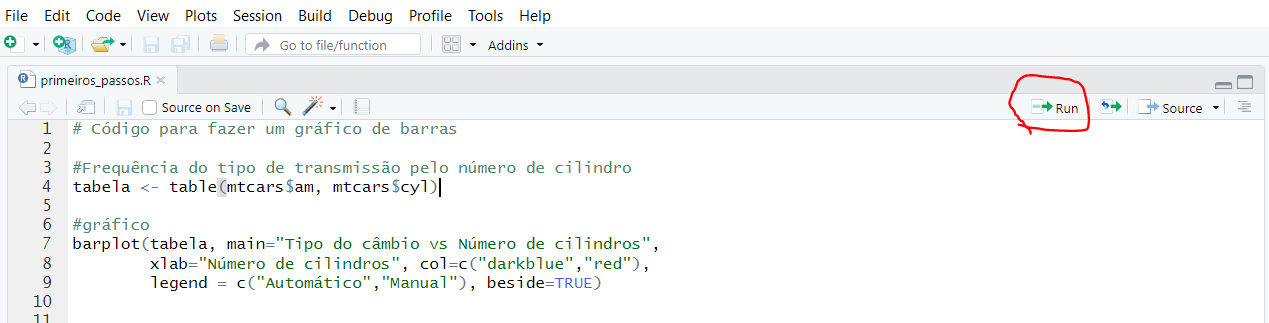
\includegraphics{imagens/3_run.png}

Essa ordem pode ser para executar apenas uma linha de código, um
conjunto de linhas ou até mesmo todo o seu \emph{script}.

Você escolhe!

O que vai definir a parte do código que será executada?

\begin{itemize}
\tightlist
\item
  Depende do que está selecionado pelo seu \emph{mouse}!
\end{itemize}

Por exemplo, se você selecionar todas as linhas do script e pedir para
executar, todo o script será executado.

Se você selecionar só uma parte, só essa parte irá rodar.

E se você não selecionar nada?

Aí o R irá executar apenas a linha onde está o cursor do \emph{mouse}
(como na imagem acima).

\hypertarget{luxf3gica-de-programauxe7uxe3o-no-r}{%
\section{Lógica de programação no
R}\label{luxf3gica-de-programauxe7uxe3o-no-r}}

A linguagem R é orientada a objetos e, na prática, isso significa que
tudo no R será um objeto.

Imagine que esse ``objeto'' é uma variável capaz de armazenar um valor
ou uma estrutura de dados. Por exemplo:

\begin{Shaded}
\begin{Highlighting}[]
\NormalTok{variavel1<-}\StringTok{ }\DecValTok{5}
\NormalTok{dataset1 <-}\StringTok{ }\NormalTok{cars}
\end{Highlighting}
\end{Shaded}

Na primeira linha do código eu estou atribuindo o valor 5 para o
\textbf{objeto} ``variavel1'', criado por mim.

O \textbf{operador de atribuição} é representado pelo
\texttt{\textless{}-}.

Você vai escolher o nome que mais fizer mais sentido para o seu objeto,
de forma que fique fácil de saber do que se trata.

Seguindo o mesmo raciocínio, eu paguei um conjunto de dados do R, que se
chama \texttt{cars} e atribui esse conjunto para o \textbf{objeto}
\texttt{dataset1}.

Então, agora o \texttt{dataset1} recebeu a estrutura de dados que estava
no dataset \texttt{cars} e os dois objetos terão o mesmo valor.

\hypertarget{as-funuxe7uxf5es-no-r}{%
\subsection{As funções no R}\label{as-funuxe7uxf5es-no-r}}

No R existem várias funções já pré-definidas. Elas servem para facilitar
trabalhos que são feitos repetidamente por muitas pessoas.

Imagine que existe um trabalho repetitivo que várias pessoas precisem
fazer.

Agora imagine que alguém já escreveu todo o passo a passo desse trabalho
repetitivo e você só precisará usar a função que essa pessoa escreveu.

Por exemplo, calcular a média aritmética é um trabalho que muitos
usuários do R vão usar, então já existe uma função para isso.

Essa função é a \texttt{mean()}.

Para usar uma função, você vai inserir dentro da função os
\textbf{argumentos} necessários.

Para calcular a média, o único argumento necessário são os números dos
quais você quer saber a média.

\begin{Shaded}
\begin{Highlighting}[]
\NormalTok{numeros <-}\StringTok{ }\DecValTok{10}\OperatorTok{:}\DecValTok{15}  \CommentTok{# estou atribuindo os números 10, 11, 12, 13, 14 e 15 para o objeto "numeros"}
\NormalTok{numeros           }\CommentTok{# pedi para o R imprimir no Console o objeto "numeros" }
\end{Highlighting}
\end{Shaded}

\begin{verbatim}
## [1] 10 11 12 13 14 15
\end{verbatim}

\begin{Shaded}
\begin{Highlighting}[]
\KeywordTok{mean}\NormalTok{(numeros)     }\CommentTok{# pedi para o R imprimir a média do objeto "numeros"}
\end{Highlighting}
\end{Shaded}

\begin{verbatim}
## [1] 12.5
\end{verbatim}

obs.: Sempre que você usar uma \# (hashtag) em seu código, o R irá
ignorar o que está à direita da Hashtag. Isso é muito útil para que você
faça \textbf{comentários} no seu código. Isso vai facilitar muito quando
você for ler o código depois de alguns dias que escreveu. E também será
extremamente útil se outra pessoa precisar ler o seu código.

\textbf{O R possui milhares e milhares de funções já prontas que irão
nos ajudar muito no desenvolvimento de nossos projetos.}

Para você saber qual a função que irá fazer o que você está precisando,
sugiro que procure no Google. Por exemplo:

Caso você queira calcular a mediana dos seus dados, coloque no Google:
\emph{R como calcular a mediana}.

E com dois cliques você irá descobrir que deve usar a função
\textbf{median()}

\hypertarget{objetos}{%
\section{Objetos}\label{objetos}}

Cada objeto irá ter uma \textbf{Classe}. Ela é definida pela forma do
objeto e será muito importante na maneira que o objeto será manipulado
pelas funções.

Existem 5 classes básicas (atômicas) para um objeto no R:

\begin{itemize}
\tightlist
\item
  Caractere (\emph{character})
\item
  Números reais (\emph{numeric})
\item
  Inteiros (\emph{integer})
\item
  Números complexos (\emph{complex})
\item
  Verdadeiro/Falso (\emph{logical})
\end{itemize}

Para descobrir qual é a \textbf{Classe} do objeto, podemos usar a função
class().

\begin{Shaded}
\begin{Highlighting}[]
\KeywordTok{class}\NormalTok{(}\StringTok{"Essa é uma frase."}\NormalTok{)}
\end{Highlighting}
\end{Shaded}

\begin{verbatim}
## [1] "character"
\end{verbatim}

\begin{Shaded}
\begin{Highlighting}[]
\KeywordTok{class}\NormalTok{(}\FloatTok{5.6761}\NormalTok{)}
\end{Highlighting}
\end{Shaded}

\begin{verbatim}
## [1] "numeric"
\end{verbatim}

\begin{Shaded}
\begin{Highlighting}[]
\KeywordTok{class}\NormalTok{(}\OtherTok{TRUE}\NormalTok{)}
\end{Highlighting}
\end{Shaded}

\begin{verbatim}
## [1] "logical"
\end{verbatim}

\textbf{O texto deve sempre estar entre aspas. Assim o R irá entender
que é um texto e não um objeto.}

Por exemplo:

\begin{Shaded}
\begin{Highlighting}[]
\NormalTok{texto <-}\StringTok{ "palavra"} \CommentTok{#aqui estou atribuindo "palavra" para o objeto texto. }
                \CommentTok{#Como eu coloquei o texto entre aspas, o R saberá que é um texto e não um objeto}
\NormalTok{texto}
\end{Highlighting}
\end{Shaded}

\begin{verbatim}
## [1] "palavra"
\end{verbatim}

Porém, quando escrevo \emph{palavra} sem as aspas, o R entenderá que eu
estou me referindo ao objeto \texttt{palavra}, porém ele não foi criado
e não existe.

\begin{Shaded}
\begin{Highlighting}[]
\NormalTok{palavra        }\CommentTok{# o R irá acusar erro, porque não existe um objeto chamado palavra.}
\end{Highlighting}
\end{Shaded}

\begin{verbatim}
## Error in eval(expr, envir, enclos): objeto 'palavra' não encontrado
\end{verbatim}

\hypertarget{vetores}{%
\section{Vetores}\label{vetores}}

\textbf{Vetor} é um conjunto de valores da mesma classe. Por exemplo:

\begin{Shaded}
\begin{Highlighting}[]
\NormalTok{inteiros <-}\StringTok{ }\KeywordTok{c}\NormalTok{(}\DecValTok{1}\NormalTok{,}\DecValTok{3}\NormalTok{,}\DecValTok{5}\NormalTok{,}\DecValTok{6}\NormalTok{) }\CommentTok{#A função "c" irá organizar os valores em vetor. }
                       \CommentTok{# Os elementos do vetor são separados por vírgula.}
                      \CommentTok{# veja que todos os valores tem a mesma classe - a classe }
                      \CommentTok{# de números inteiros.}


\NormalTok{logicos <-}\StringTok{ }\KeywordTok{c}\NormalTok{(}\OtherTok{TRUE}\NormalTok{,}\OtherTok{FALSE}\NormalTok{,}\OtherTok{TRUE}\NormalTok{) }\CommentTok{#Vetor com valores lógicos verdadeiro/falso}
\NormalTok{logicos <-}\StringTok{ }\KeywordTok{c}\NormalTok{(T,F,T) }\CommentTok{#Você pode escrever TRUE ou somente T,  }
                    \CommentTok{# FALSE ou somente F e o R irá entender }
                    \CommentTok{# que se trata de valores lógicos}
\end{Highlighting}
\end{Shaded}

Quando escrevemos os valores lógicos TRUE ou T e FALSE ou F, o R já sabe
que são valores lógicos. Portanto, não precisamos colocá-los entre
aspas.

\hypertarget{matrizes}{%
\section{Matrizes}\label{matrizes}}

Imagine alguns vetores do mesmo tamanho:

\begin{Shaded}
\begin{Highlighting}[]
\NormalTok{vetor1 <-}\StringTok{ }\KeywordTok{c}\NormalTok{(}\DecValTok{0}\NormalTok{,}\DecValTok{1}\NormalTok{,}\DecValTok{2}\NormalTok{,}\DecValTok{3}\NormalTok{)}
\NormalTok{vetor2 <-}\StringTok{ }\KeywordTok{c}\NormalTok{(}\DecValTok{3}\NormalTok{,}\DecValTok{2}\NormalTok{,}\DecValTok{1}\NormalTok{,}\DecValTok{0}\NormalTok{)}
\NormalTok{vetor3 <-}\StringTok{ }\KeywordTok{c}\NormalTok{(}\DecValTok{1}\NormalTok{,}\DecValTok{1}\NormalTok{,}\DecValTok{1}\NormalTok{,}\DecValTok{1}\NormalTok{)}
\end{Highlighting}
\end{Shaded}

Uma matriz é um conjunto de vetores do mesmo tamanho. Ou uma tabela com
linhas e colunas. Como você preferir!

\begin{Shaded}
\begin{Highlighting}[]
\CommentTok{#a função matrix é usada para criar uma matriz}
\CommentTok{#o primeiro argumento da função matrix são os dados da matriz}
\CommentTok{#além disso o argumento "ncol" irá informar que desejamos formar 3 colunas.}
\CommentTok{#Assim, cada vetor definido anteriormente será uma coluna da matriz}
\KeywordTok{matrix}\NormalTok{(}\KeywordTok{cbind}\NormalTok{(vetor1,vetor2,vetor3),}\DataTypeTok{ncol=}\DecValTok{3}\NormalTok{)}
\end{Highlighting}
\end{Shaded}

\begin{verbatim}
##      [,1] [,2] [,3]
## [1,]    0    3    1
## [2,]    1    2    1
## [3,]    2    1    1
## [4,]    3    0    1
\end{verbatim}

Outro exemplo:

\begin{Shaded}
\begin{Highlighting}[]
\CommentTok{#Foram definidos os valores de 1 a 6 no argumento de dados da função.}
\CommentTok{#e também foi definido que número de linhas (nrow) igual a 2}
\CommentTok{#e o número de colunas igual a 3.}
\KeywordTok{matrix}\NormalTok{(}\DecValTok{1}\OperatorTok{:}\DecValTok{6}\NormalTok{, }\DataTypeTok{nrow =} \DecValTok{2}\NormalTok{, }\DataTypeTok{ncol =} \DecValTok{3}\NormalTok{)}
\end{Highlighting}
\end{Shaded}

\begin{verbatim}
##      [,1] [,2] [,3]
## [1,]    1    3    5
## [2,]    2    4    6
\end{verbatim}

Importante: todas as colunas de uma \textbf{matriz} possuem a
\textbf{mesma classe}. Ou seja, são todas numéricas ou são todas lógicas
ou são todas caracteres, etc.

\hypertarget{listas}{%
\section{Listas}\label{listas}}

Você vai usar bastante as \textbf{listas} em seus trabalhos. A principal
característica delas é aceitar elementos de diferentes classes. Além
disso, podem armazenar vetores e matrizes em um único objeto.

Exemplo:

\begin{Shaded}
\begin{Highlighting}[]
\NormalTok{vetor1 <-}\StringTok{ }\KeywordTok{c}\NormalTok{(}\OtherTok{TRUE}\NormalTok{,}\OtherTok{FALSE}\NormalTok{,}\OtherTok{TRUE}\NormalTok{)        }\CommentTok{#Vetor com valores lógicos}
\NormalTok{vetor2 <-}\StringTok{ }\KeywordTok{c}\NormalTok{(}\DecValTok{2}\NormalTok{,}\DecValTok{3}\NormalTok{,}\DecValTok{4}\NormalTok{,}\DecValTok{5}\NormalTok{,}\DecValTok{6}\NormalTok{,}\DecValTok{7}\NormalTok{,}\DecValTok{8}\NormalTok{,}\DecValTok{9}\NormalTok{)        }\CommentTok{#Vetor com valores inteiros}
\NormalTok{valor_texto <-}\StringTok{ "Esse é um texto."}   \CommentTok{#Elemento da classe character}
\NormalTok{lista <-}\StringTok{ }\KeywordTok{list}\NormalTok{(vetor1,vetor2,valor_texto)}
\NormalTok{lista}
\end{Highlighting}
\end{Shaded}

\begin{verbatim}
## [[1]]
## [1]  TRUE FALSE  TRUE
## 
## [[2]]
## [1] 2 3 4 5 6 7 8 9
## 
## [[3]]
## [1] "Esse é um texto."
\end{verbatim}

\hypertarget{fatores}{%
\section{Fatores}\label{fatores}}

Até agora usamos em nossos exemplos valores lógicos (TRUE/FALSE),
valores numéricos ou de texto (\emph{character}). Porém, é essencial
conhecer outra classe de valores: \textbf{os fatores}.

\textbf{Fator é a classe das variáveis categóricas.}

Uma variável categórica pode ser ordenada, como a renda: salários até
R\$ 5.000, entre R\$ 5.001 e 10.000 e acima de R\$ 10.000.

Ou podemos ter categorias que não possuem nenhuma ordem, como cursos:
Administração, Economia, Ciência Contábeis.

Nos dois exemplos, as variáveis \emph{renda} e \emph{cursos} poderiam
assumir a classe ``factor'' em nossas análises.

Também seria possível classificar renda e cursos (ou qualquer variável
categórica) como uma variável de texto (\emph{character}).

\textbf{Então para o que serve a classe dos fatores?}

Sempre que você tiver poucos valores únicos para uma variável, prefira a
classificação de fator à \emph{character}. Essa opção irá otimizar o
armazenamento dos dados e também será necessária para utilizar algumas
funções do R com seus dados.

Exemplo:

Uma pergunta aberta em um questionário irá gerar várias respostas
diferentes, então não há sentido nenhum em classificar as respostas em
categorias. Portanto, a classificação adequada é \emph{character}.

Porém, caso o respondente tenha que escolher uma resposta entre algumas
opções disponíveis para esse questionário, a melhor classificação da
variável seria como fator.

\textbf{O R sempre irá assumir uma classificação para a sua variável e,
a priori, você não precisará fazer essa classificação. Ela só é
necessária quando a classificação automática feita pelo R for indevida
para o seu caso.}

\hypertarget{coeruxe7uxe3o-de-classes}{%
\section{Coerção de classes}\label{coeruxe7uxe3o-de-classes}}

Em alguns casos, você pode precisar alterar a classe de objetos.

Suponha, por exemplo, que você criou o seguinte vetor x.

\begin{Shaded}
\begin{Highlighting}[]
\NormalTok{x<-}\KeywordTok{c}\NormalTok{(}\DecValTok{0}\NormalTok{,}\DecValTok{1}\NormalTok{,}\DecValTok{0}\NormalTok{,}\DecValTok{1}\NormalTok{,}\DecValTok{1}\NormalTok{)}
\end{Highlighting}
\end{Shaded}

O R irá automaticamente entender que o vetor \emph{x} é \emph{numeric}

\begin{Shaded}
\begin{Highlighting}[]
\KeywordTok{class}\NormalTok{(x)}
\end{Highlighting}
\end{Shaded}

\begin{verbatim}
## [1] "numeric"
\end{verbatim}

Porém, pode ser que você precise desse vetor como \emph{integer}
(números inteiros) ou \emph{logical} (verdadeiro/falso). Por definição 0
seria FALSO e 1 seria VERDADEIRO.

Para alterar a classe de um objeto por coerção, basta você usar uma
função de coerção. As função são definidas por \textbf{as.} +
\emph{classe que o objeto vai assumir}.

Ou seja: as.integer, as.logical, as.numeric, as.factor as.complex ou
as.\emph{character}.

Para o exemplo acima, teríamos:

\begin{Shaded}
\begin{Highlighting}[]
\KeywordTok{as.integer}\NormalTok{(x)}
\end{Highlighting}
\end{Shaded}

\begin{verbatim}
## [1] 0 1 0 1 1
\end{verbatim}

\begin{Shaded}
\begin{Highlighting}[]
\KeywordTok{as.logical}\NormalTok{(x)}
\end{Highlighting}
\end{Shaded}

\begin{verbatim}
## [1] FALSE  TRUE FALSE  TRUE  TRUE
\end{verbatim}

\textbf{Dica importante}: Muito cuidado ao converter objetos
classificados como FATORES para NUMÉRICOS. Para fazer isso sem perder
informação, você precisa converter primeiramente para \emph{character}
e, posteriormente, para \emph{numeric}.

\hypertarget{valores-faltantes}{%
\section{Valores faltantes}\label{valores-faltantes}}

Os valores faltantes, também chamados de \textbf{missing values} são
representados por \emph{NA} ou \emph{NaN}.

Eles não irão influenciar a classe de um objeto, por exemplo:

\begin{Shaded}
\begin{Highlighting}[]
\NormalTok{x<-}\KeywordTok{c}\NormalTok{(}\DecValTok{1}\NormalTok{,}\DecValTok{2}\NormalTok{,}\OtherTok{NA}\NormalTok{,}\DecValTok{1}\NormalTok{,}\DecValTok{0}\NormalTok{) }\CommentTok{#apesar de ser representado por duas letras, pelo padrão do R, ele saberá que não se trata de um texto e sim de valores faltantes.}
\KeywordTok{class}\NormalTok{(x)}
\end{Highlighting}
\end{Shaded}

\begin{verbatim}
## [1] "numeric"
\end{verbatim}

\hypertarget{data-frames}{%
\section{Data Frames}\label{data-frames}}

Provavelmente esse é o objeto mais usado no R. É similar a uma matriz,
porém com mais possibilidades.

Os \textbf{Data Frames} são tabelas que aceitam colunas de todas as
classes. Por exemplo, podemos ter uma coluna com classe \emph{numeric},
outra \emph{logical} e outra \emph{character}. Isso não é possível em
uma matriz, onde todas as colunas devem ter a mesma classe.

Cada coluna em um \emph{Data Frame} terá um nome. É altamente
recomendável que você atribua nomes que realmente representem a variável
ali contida. Ou seja, \textbf{evite} nomes como X1, X2, X3, etc.

Também é possível atribuir nomes para as linhas de seu \textbf{data
frame}.

É muito comum que você importe seus dados/tabela para o R, porém veja
como você pode criar um \emph{data frame} de forma bem simples:

\begin{Shaded}
\begin{Highlighting}[]
\NormalTok{meus_dados <-}\StringTok{ }\KeywordTok{data.frame}\NormalTok{(}\DataTypeTok{produto=}\KeywordTok{c}\NormalTok{(}\StringTok{"roda"}\NormalTok{,}\StringTok{"pneu"}\NormalTok{,}\StringTok{"suspensão"}\NormalTok{), }\DataTypeTok{preco =} \KeywordTok{c}\NormalTok{(}\DecValTok{30}\NormalTok{,}\DecValTok{20}\NormalTok{,}\DecValTok{15}\NormalTok{), }\DataTypeTok{esta_disponivel =} \KeywordTok{c}\NormalTok{(T, T, F))}
\NormalTok{meus_dados}
\end{Highlighting}
\end{Shaded}

\begin{verbatim}
##     produto preco esta_disponivel
## 1      roda    30            TRUE
## 2      pneu    20            TRUE
## 3 suspensão    15           FALSE
\end{verbatim}

O \textbf{data frame} criado acima possui variáveis de texto, numérica e
lógica.

\hypertarget{names}{%
\section{Names}\label{names}}

Os \textbf{names} são muito úteis na manipulação dos dados contidos nas
matrizes, listas ou \emph{data frames}.

Por exemplo, no \emph{data frame} \textbf{meus\_dados} criado no item
anterior, foi definido que o nome das variáveis são: produto, preco e
esta\_disponivel.

Isso pode ser identificado pela função \texttt{names()}

\begin{Shaded}
\begin{Highlighting}[]
\KeywordTok{names}\NormalTok{(meus_dados)}
\end{Highlighting}
\end{Shaded}

\begin{verbatim}
## [1] "produto"         "preco"           "esta_disponivel"
\end{verbatim}

Veremos como podemos usar os nomes das colunas no capítulo de
manipulação de dados.

Para alterar os nomes das colunas ou linhas de um \emph{data frame},
usa-se as funções \texttt{names()} e \texttt{row.names()}.

\begin{Shaded}
\begin{Highlighting}[]
\KeywordTok{names}\NormalTok{(meus_dados)<-}\KeywordTok{c}\NormalTok{(}\StringTok{"novo_nome"}\NormalTok{,}\StringTok{"preco"}\NormalTok{,}\StringTok{"esta_disponivel"}\NormalTok{) }\CommentTok{#alterando o nome da 1a coluna}
\NormalTok{meus_dados}
\end{Highlighting}
\end{Shaded}

\begin{verbatim}
##   novo_nome preco esta_disponivel
## 1      roda    30            TRUE
## 2      pneu    20            TRUE
## 3 suspensão    15           FALSE
\end{verbatim}

www.luisotavio.pro

\hypertarget{instalar-pacotes-no-r}{%
\chapter{Instalar Pacotes no R}\label{instalar-pacotes-no-r}}

O R é uma linguagem inicialmente dedicada a métodos estatísticos. Como a
Estatística é uma ciência extremamente ampla, são os pacotes que
permitem o R ser um software tão completo!

Olha só:

O R é utilizado por pessoas da área de economia, previsões do tempo,
área de saúde, demografia, machine learning, deep learning e várias
outras\ldots{}

Sendo que cada uma das áreas citadas ainda tem vários subnichos.

Então o que acontece é o seguinte:

existem milhares de pessoas ao redor do mundo que são muito boas em suas
áreas e criam pacotes dentro do R para atender demandas específicas.
Que, geralmente, ainda não tinham sido solucionadas de forma eficaz.

Isso só é possível porque o R é um software Open Source. Isso significa
que as pessoas podem contribuir para melhorar as funcionalidades do
programa! Com certeza, isso é determinante para o R ser tão completo.

O que estou falando é que se um especialista da sua área de uma
universidade renomada publica um pacote no R, ele estará disponível para
você usar no seu computador! Gratuitamente.

Agora que você já entendeu o contexto, vamos definir o que é um pacote
do R:

\textbf{Um Pacote é um conjunto de funções dentro do R, geralmente
relacionados a um tema específico.}

Além disso, os pacotes também têm uma documentação. Essa documentação
explica para o que serve cada função do pacote. Te explica como usar
cada função e ainda fornece exemplos práticos de uso.

\hypertarget{como-instalar-um-pacote-no-r-ou-rstudio}{%
\section{Como instalar um pacote no R ou
RStudio}\label{como-instalar-um-pacote-no-r-ou-rstudio}}

Quando fazemos o download do R, também já estamos baixando os pacotes
considerados básicos.

Mas muitas vezes você vai precisar de um pacote específico, pode ser
para fazer um gráfico mais bonito, para trabalhar com datas de uma forma
mais eficiente ou para trabalhar com mais qualidade com o próprio tema
do seu projeto.

E para isso vamos fazer o download desse pacote, é muito simples!

O \textbf{ggplot2} é um pacote muito usado para fazer gráficos mais
elaborados, com grande capacidade de personalização.

Vamos usá-lo aqui como exemplo.

Existem três maneiras comuns para se instalar um pacote.

As duas primeiras são as maneiras mais tradicionais. Já a terceira será
utilizada quando o pacote não estiver disponível para download na rede
do R.

\hypertarget{usando-o-botuxe3o-de-instalauxe7uxe3o}{%
\subsection{Usando o botão de
instalação}\label{usando-o-botuxe3o-de-instalauxe7uxe3o}}

Essa forma é muito intuitiva, clique na aba ``Packages'' (veja na
imagem) e depois em ``Install''. Irá abrir uma tela para você escolher o
pacote que deseja instalar.

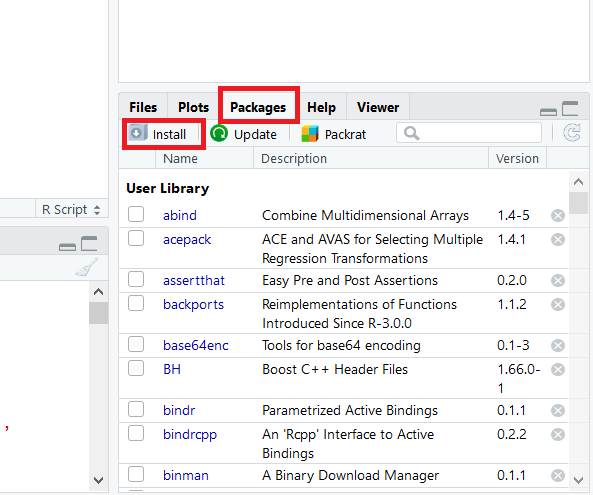
\includegraphics{imagens/4_pacotes_botao_instalacao.png}

Escreva o nome o pacote e clique em ``Install''. Simples assim! Mas
ainda falta um detalhe.

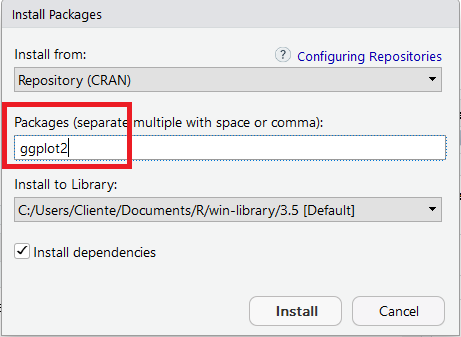
\includegraphics{imagens/4_pacotes_install.png}

Agora o pacote já está instalado no R, em sua biblioteca.

\textbf{Mas falta um detalhe, precisamos ir lá na biblioteca e buscar
esse pacote!}

Para carregar o pacote instalado, basta executar o seguinte código:

\begin{Shaded}
\begin{Highlighting}[]
\KeywordTok{library}\NormalTok{(ggplot2) }\CommentTok{#Esse exemplo irá carregar o pacote ggplot2, }
\CommentTok{#então coloque o nome do pacote que você instalou e deseja carregar.}
\end{Highlighting}
\end{Shaded}

\hypertarget{usando-o-comando-de-instalauxe7uxe3o}{%
\subsection{Usando o comando de
instalação}\label{usando-o-comando-de-instalauxe7uxe3o}}

O primeiro passo é escrever o comando
\texttt{install.packages("ggplot2")} e executar o código!

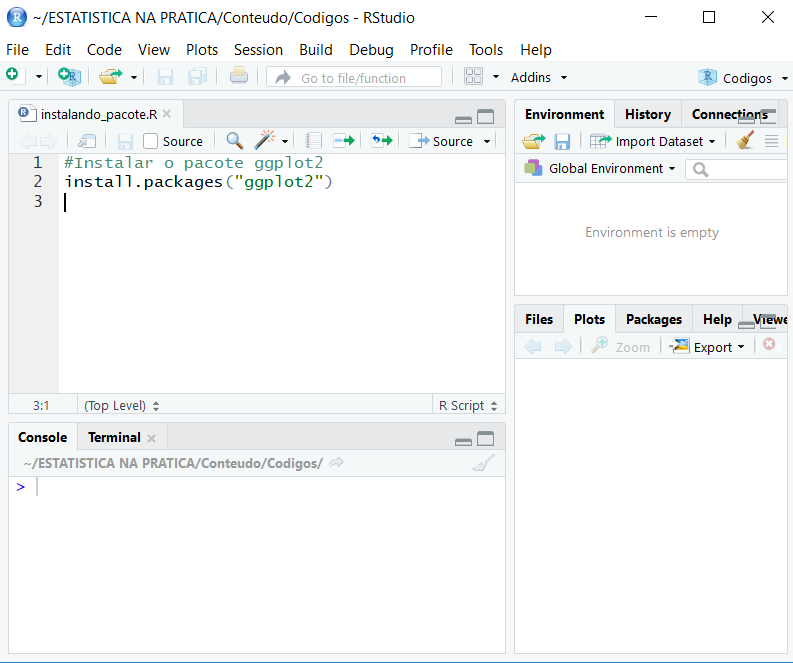
\includegraphics{imagens/4_pacotes_comando_install.png}

Execute o código:

\begin{Shaded}
\begin{Highlighting}[]
\KeywordTok{install.packages}\NormalTok{(}\StringTok{"ggplot2"}\NormalTok{) }\CommentTok{#Esse exemplo irá instalar o pacote ggplot2, }
\CommentTok{# então coloque o nome do pacote que você deseja instalar.}
\end{Highlighting}
\end{Shaded}

Depois que o código for executado, o pacote será instalado.

Isso quer dizer que o pacote está instalado no R, em sua biblioteca.

Mas também precisamos ir lá na biblioteca e buscar esse pacote.

\begin{Shaded}
\begin{Highlighting}[]
\KeywordTok{library}\NormalTok{(}\StringTok{"ggplot2"}\NormalTok{) }\CommentTok{#Esse exemplo irá carregar o pacote ggplot2,}
\CommentTok{# então coloque o nome do pacote que você instalou e deseja carregar.}
\end{Highlighting}
\end{Shaded}

\hypertarget{usando-o-devtools}{%
\subsection{Usando o Devtools}\label{usando-o-devtools}}

A rede onde estão armazenados os pacotes do R é conhecida como CRAN.

Em alguns casos, o pacote que você deseja instalar não estará disponível
no CRAN.

Há uma maneira muito simples de resolver isso. Vários desenvolvedores de
pacotes os armazenam no \href{https://www.github.com}{Github}.

Imagine que você esteja procurando no Google como solucionar um problema
e encontre um pacote que resolverá sua questão, mas não está disponível
no CRAN.

Provavelmente o pacote está disponível no \textbf{Github} e poderá ser
instalado usando o pacote \textbf{Devtools}.

O primeiro passo é instalar o Devtools (que está disponível para ser
instalada normalmente pela rede do R).

\begin{Shaded}
\begin{Highlighting}[]
\KeywordTok{install.packages}\NormalTok{(}\StringTok{"devtools"}\NormalTok{)}
\end{Highlighting}
\end{Shaded}

\textbf{O script a seguir deve ser adaptado ao pacote que você quiser
instalar.} Você o encontrará na página do Github do pacote que irá
instalar. Provavelmente na seção \textbf{Readme}.

Para exemplificar, vou instalar o pacote \textbf{rCharts}, que não está
disponível para instalação no CRAN usando os primeiros métodos falados
aqui.

\begin{Shaded}
\begin{Highlighting}[]
\KeywordTok{library}\NormalTok{(devtools)}
\KeywordTok{install_github}\NormalTok{(}\StringTok{'ramnathv/rCharts'}\NormalTok{) }\CommentTok{# ramnathv é o usuário do Github que criou o pacote rCharts}
\end{Highlighting}
\end{Shaded}

Pronto. O comando acima irá instalar o pacote rCharts que não pode ser
instalado pelas duas primeiras formas mostradas.

Seguindo o mesmo raciocínio anterior, você precisará chamar o pacote
antes de utilizá-lo:

\begin{Shaded}
\begin{Highlighting}[]
\KeywordTok{library}\NormalTok{(rCharts)}
\end{Highlighting}
\end{Shaded}

www.luisotavio.pro

\hypertarget{como-ler-ou-salvar-seus-dados}{%
\chapter{Como ler ou salvar seus
dados}\label{como-ler-ou-salvar-seus-dados}}

Nesse capítulo vou te apresentar as principais formas de
\textbf{importar os seus dados para o R}.

Em alguns casos específicos, a importação dos dados pode depender de
pacotes desenvolvidos especialmente para o caso. Aqui vou abordar a
importação de arquivos de texto, CSV ou Excel.

Vou falar sobre a importação de dados do Excel no final deste capítulo.
Porém, caso você queira importar poucas abas de uma planilha do Excel,
recomendo que você a salve como arquivo TXT e faça a importação usando o
método a seguir.

\hypertarget{como-importar-uma-tabela-em-arquivo-txt-ou-csv-para-o-rstudio}{%
\section{Como importar uma tabela em arquivo txt ou csv para o
RStudio}\label{como-importar-uma-tabela-em-arquivo-txt-ou-csv-para-o-rstudio}}

\hypertarget{muxe9todo-sem-nenhuma-linha-de-cuxf3digo}{%
\subsection{Método sem nenhuma linha de
código}\label{muxe9todo-sem-nenhuma-linha-de-cuxf3digo}}

Após aplicar esse método, você terá importado seus dados em segundos e,
além disso, o R te mostrará qual o código ele executou para abrir a sua
tabela! Ou seja, uma ótima oportunidade pra você entender melhor sobre a
linguagem.

\textbf{Passo 1 - Na parte ``Enviroment'' clique em Import Dataset
-\textgreater{} From Txt (readr)}

Lembre-se que os seus dados devem estar salvos no formato txt ou csv.

\begin{figure}
\centering
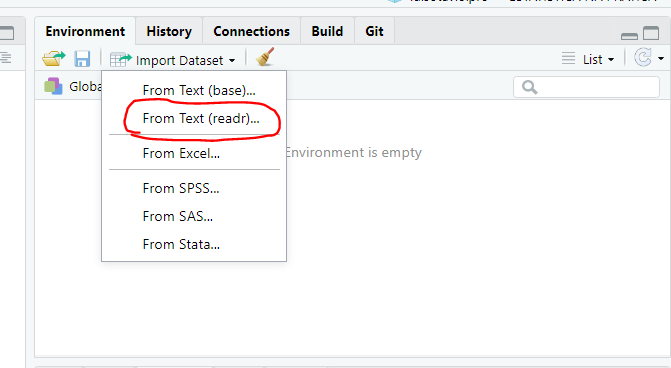
\includegraphics{imagens/5_importacao1.png}
\caption{Importar dados no R-RStudio}
\end{figure}

Para ler os dados vamos usar a biblioteca \texttt{readr}, então, caso
você ainda não tenha ela instalada em seu computador, o RStudio irá
solicitar a sua instalação.

\textbf{Passo 2 - Instale a biblioteca \texttt{readr}, caso ela já não
esteja instalada}

\begin{figure}
\centering
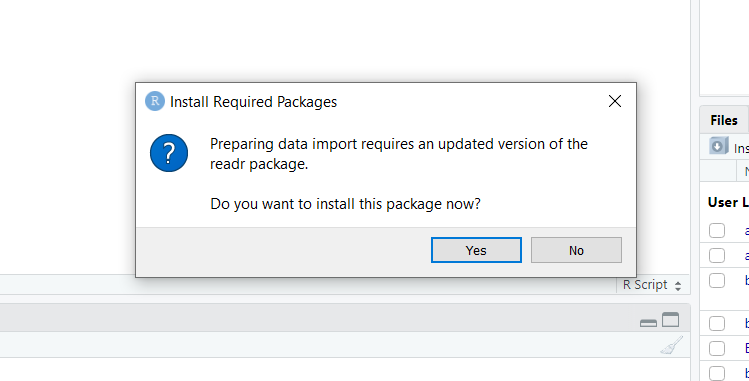
\includegraphics{imagens/5_importacao2.png}
\caption{Importar dados no R-RStudio}
\end{figure}

Clique em ``Yes'' e aguarde a instalação.

\textbf{Passo 3 - Ajustes para importar a sua tabela}

\begin{figure}
\centering
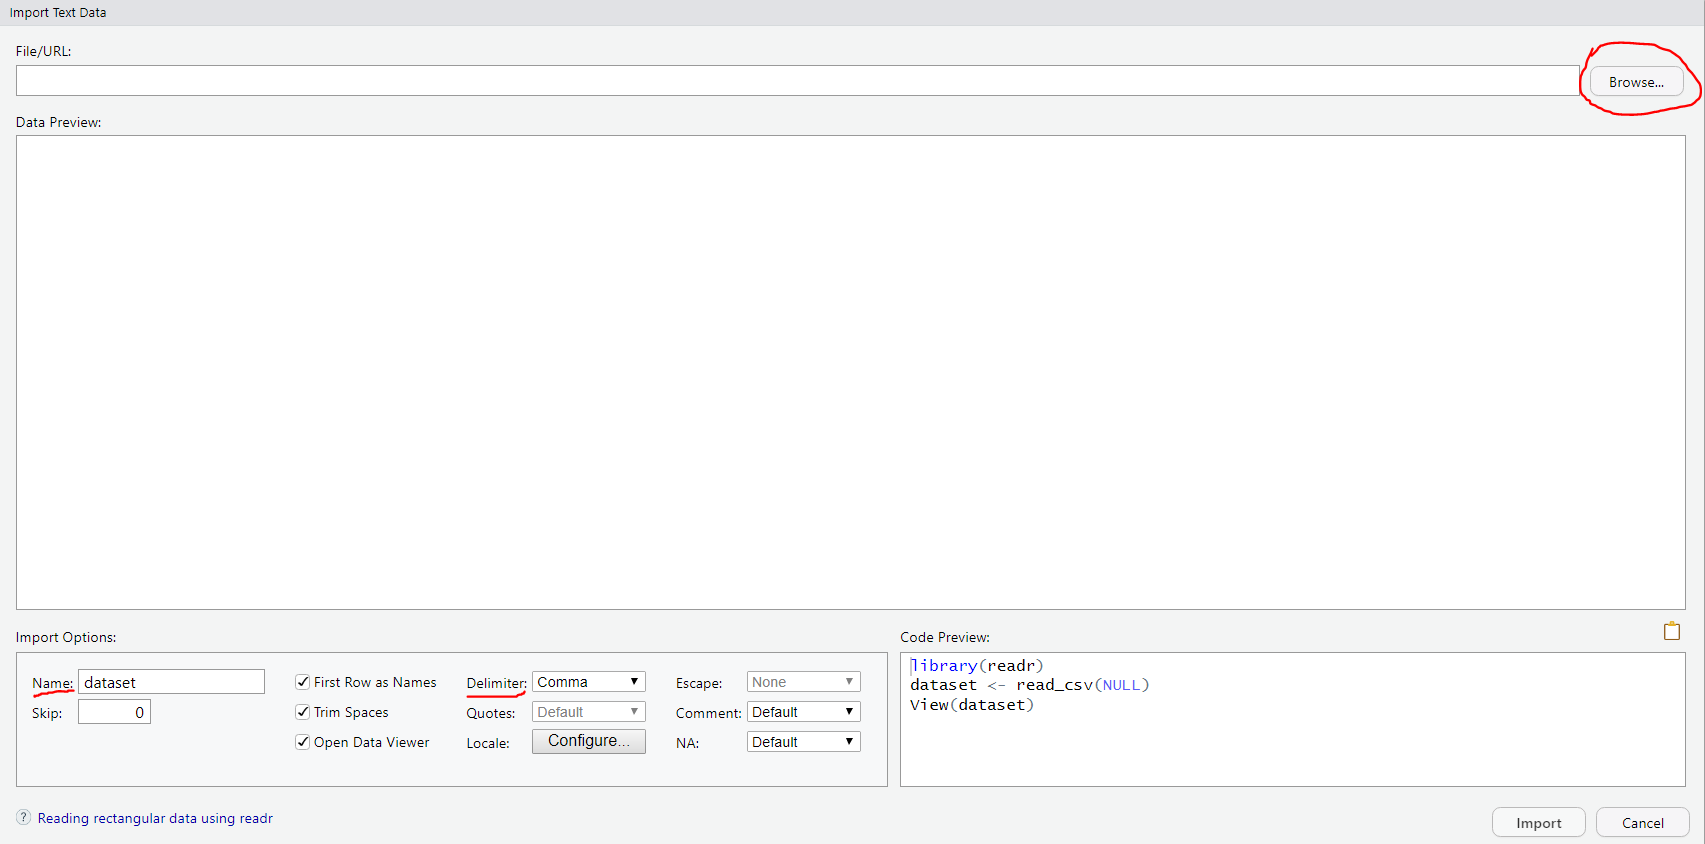
\includegraphics{imagens/5_importacao3.png}
\caption{Importar dados no R-RStudio}
\end{figure}

Primeiramente, clique em ``\emph{Browse}'' e selecione o arquivo que
você deseje importar.

Uma pequena parte dos dados do arquivo que você selecionou irão aparecer
na sua tela, para te auxiliar na importação.

Então, agora você precisa fazer alguns ajustes para o R ler o seu
conjunto de dados (\emph{dataset}).

\textbf{O ajuste mais importante é como as suas colunas estão
separadas/delimitadas.}

É muito comum usar tabulação (tab), vírgula, ponto e vírgula ou espaço
para separar as colunas de arquivos de texto.

Mas nessa parte da importação, \textbf{você deve escolher exatamente o
mesmo delimitador que já foi utilizado em seu arquivo.}

Nessa seção, você também pode fazer vários outros ajustes, por exemplo:

\begin{itemize}
\item
  escolher o nome da tabela que será importada
\item
  definir qual se os números decimais da sua tabela estão separados por
  ponto ou vírgula. No R o separador decimal é por ponto, então caso o
  seu arquivo use vírgula, o R saberá que deve transformar pra ficar
  dentro do padrão.
\item
  alterar qual a codificação dos seus dados (ASCII, utf8, etc\ldots)
\item
  definir se a primeira linha dos seus dados é cabeçalho ou não
\end{itemize}

Note que nessa etapa, na parte de ``\textbf{Code Preview}'', o RStudio
está mostrando exatamente o código que será executado para fazer a
leitura dos seus dados.

Esse código vai alterando a medida que você muda os ajustes! (ótima
oportunidade para aprender e ir entendendo melhor o funcionamento da
linguagem).

Após realizar os ajustes necessários (que vão depender da sua própria
tabela), clique em Import

Pronto, agora os seus dados foram importados.

Você pode conferir que a sua tabela irá aparecer em ``Enviroment''. É só
clicar nela para visualizar os dados.

\hypertarget{importando-dados-com-a-funuxe7uxe3o-read.table}{%
\subsection{Importando dados com a função
read.table}\label{importando-dados-com-a-funuxe7uxe3o-read.table}}

A função mais comum para importar dados no R é a \texttt{read.table}. A
função é bem simples, vou mostrar a seguir:

\begin{Shaded}
\begin{Highlighting}[]
\NormalTok{meus_dados<-}\KeywordTok{read.table}\NormalTok{(}\DataTypeTok{file=}\StringTok{"nome_do_arquivo.txt"}\NormalTok{,}\DataTypeTok{header =} \OtherTok{TRUE}\NormalTok{,}\DataTypeTok{sep =} \StringTok{"}\CharTok{\textbackslash{}t}\StringTok{"}\NormalTok{)}
\end{Highlighting}
\end{Shaded}

Portanto, esse comando irá ler o arquivo ``nome\_do\_arquivo.txt''. Além
disso, foi informado que o arquivo possui cabeçalho (nome para cada
coluna da tabela) e está separado por tabulação, representado pelo
símbolo \texttt{"\textbackslash{}t"}.

Você pode atribuir valores para outros argumentos, como: \emph{dec}
(para definir o separador de números decimais), \emph{row.names} (para
atribuir nomes para cada linha), \emph{encoding} (definir a codificação
dos seus dados) e vários outros.

Essas opções só precisarão ser utilizadas em casos especiais, quando
seus dados não estiverem no padrão definido pelo R.

Como qualquer função no R, você terá acesso a documentação da função
executanto o comando \texttt{?read.table}.

\hypertarget{como-importar-dados-do-excel-para-o-rstudio}{%
\section{Como importar dados do Excel para o
RStudio}\label{como-importar-dados-do-excel-para-o-rstudio}}

A seguir temos 3 métodos para ler dados do Excel no RStudio. Todos são
bem simples e cada um será mais útil em um tipo de situação.

\hypertarget{copiando-os-dados-do-excel-e-importando-para-o-r.}{%
\subsection{Copiando os dados do Excel e importando para o
R.}\label{copiando-os-dados-do-excel-e-importando-para-o-r.}}

1 -- Abra o seu arquivo de Excel, selecione os dados que deseja copiar e
copie os dados (Ctrl + C).

2 -- Execute o código abaixo para importar os dados copiados no Excel.

\begin{Shaded}
\begin{Highlighting}[]
\NormalTok{meus_dados <-}\StringTok{ }\KeywordTok{read.table}\NormalTok{(}\DataTypeTok{file =} \StringTok{"clipboard"}\NormalTok{, }\DataTypeTok{sep =} \StringTok{"}\CharTok{\textbackslash{}t}\StringTok{"}\NormalTok{, }\DataTypeTok{header=}\OtherTok{TRUE}\NormalTok{)}
\end{Highlighting}
\end{Shaded}

\begin{verbatim}
## Warning in read.table(file = "clipboard", sep = "\t", header = TRUE): incomplete
## final line found by readTableHeader on 'clipboard'
\end{verbatim}

Quando copiamos os dados no Excel, eles ficam armazenados no clipboard
do nosso computador, então o que estamos fazendo é falando para o R ler
a tabela (função read.table) que estão no clipboard e atribuir essa
tabela aos ``meus\_dados''.

3 -- Pronto!

\hypertarget{importando-arquivos-do-excel-sem-usar-programauxe7uxe3o}{%
\subsection{Importando arquivos do Excel sem usar
programação}\label{importando-arquivos-do-excel-sem-usar-programauxe7uxe3o}}

Agora vamos ver como importar um arquivo do Excel para o R usando apenas
o nosso mouse, é muito simples!

1 - Na aba \textbf{``Enviroment''}, vamos clicar em \emph{Import
Dataset} e escolher \emph{From Excel}.

\begin{figure}
\centering
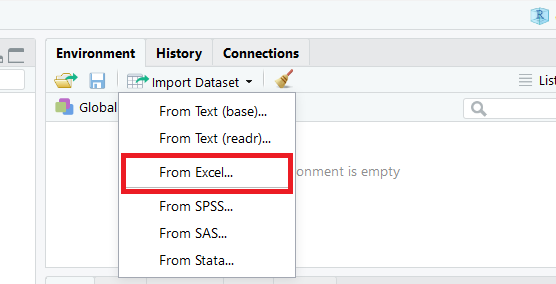
\includegraphics{imagens/5_excel1.png}
\caption{Importar dados no R-RStudio}
\end{figure}

2 -- Você provavelmente ainda não instalou o pacote \texttt{readxl},
então o RStudio vai te perguntar se deseja instalar o pacote. Confirme a
instalação.

\begin{figure}
\centering
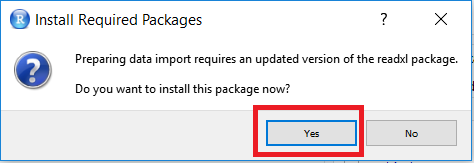
\includegraphics{imagens/5_excel2.png}
\caption{Importar dados no R-RStudio}
\end{figure}

3 - Aparecerá uma aba para você fazer a leitura dos dados desejados.
Clique em \emph{Browse} para escolher o arquivo de Excel que você irá
importar. Depois em \emph{Sheet} escolha a aba de seu arquivo onde está
a tabela que você quer importar.

(Caso queira importar várias abas é só repetir os passos, importando uma
aba de cada vez)

\begin{figure}
\centering
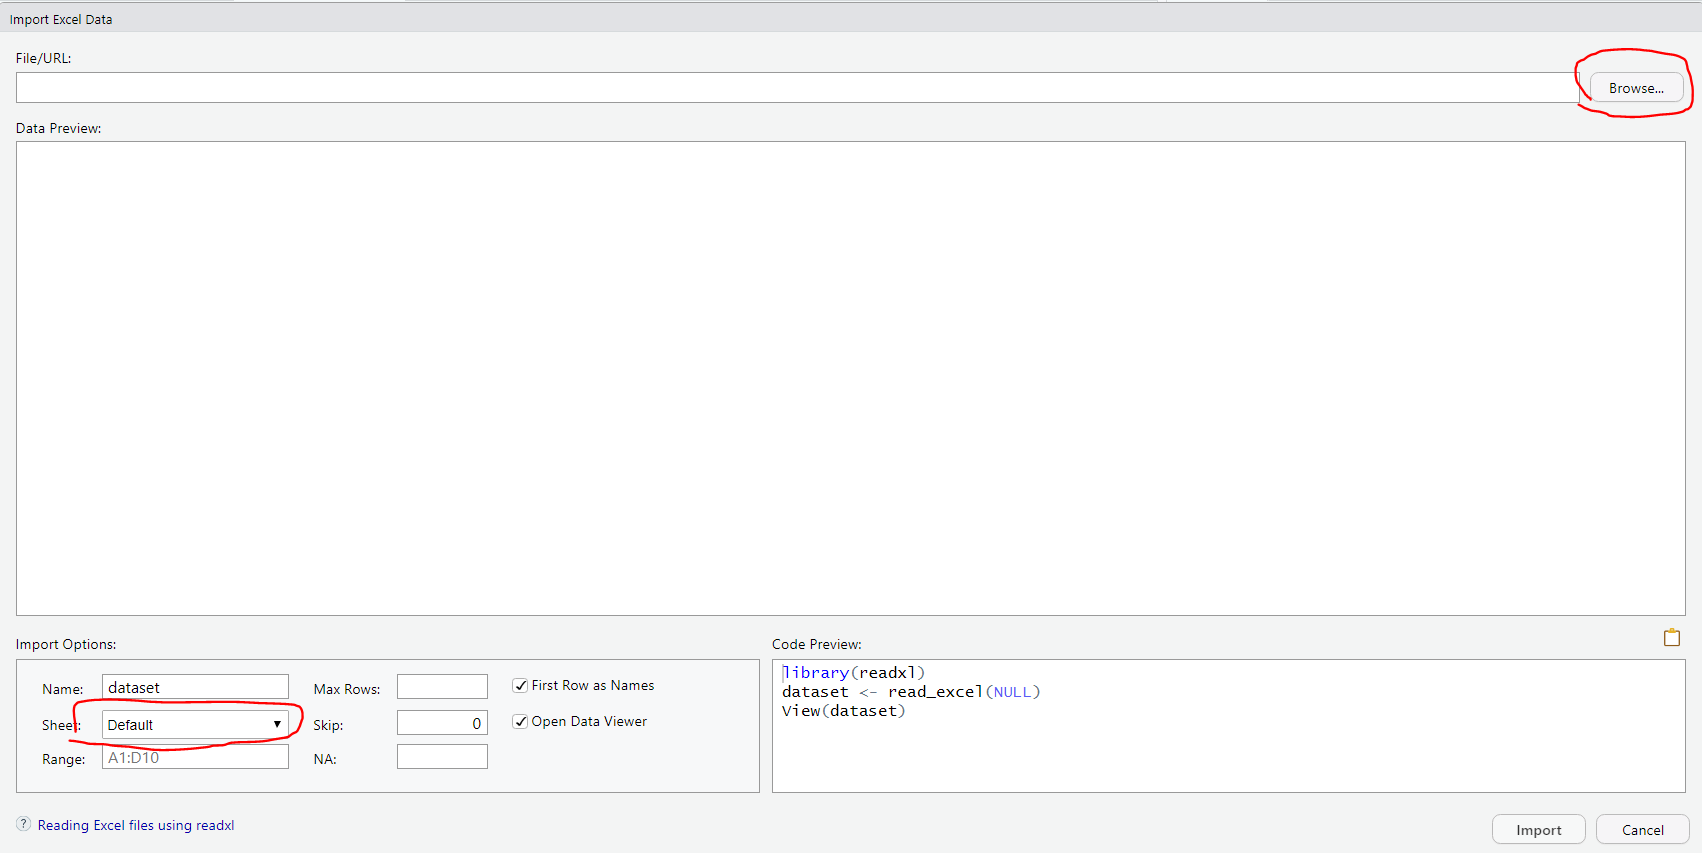
\includegraphics{imagens/5_excel3.png}
\caption{Importar dados no R-RStudio}
\end{figure}

4 -- Clique em \emph{Import}.

\hypertarget{abrir-os-dados-do-excel-no-r-usando-o-pacote-readxl}{%
\subsection{Abrir os dados do Excel no R usando o pacote
readxl}\label{abrir-os-dados-do-excel-no-r-usando-o-pacote-readxl}}

Esse método é bem parecido com o último, porém aqui vamos usar linhas de
código.

1 - Caso você ainda não tenha instalado o pacote \texttt{readxl},
execute o seguinte comando:

\begin{Shaded}
\begin{Highlighting}[]
\KeywordTok{install.packages}\NormalTok{(}\StringTok{"readxl"}\NormalTok{)}
\end{Highlighting}
\end{Shaded}

2 - Vamos carregar o pacote que iremos usar (\texttt{readxl}): Execute o
comando:

\begin{Shaded}
\begin{Highlighting}[]
\KeywordTok{library}\NormalTok{(}\StringTok{"readxl"}\NormalTok{)}
\end{Highlighting}
\end{Shaded}

3 -- Agora vamos buscar a planilha que você precisa usando a função
\texttt{read\_excel}.

Os argumentos que vamos usar na função são:

\begin{itemize}
\tightlist
\item
  o endereço e nome do seu arquivo;
\item
  a aba da planilha que você quer ler.
\end{itemize}

Excute o código:

\begin{Shaded}
\begin{Highlighting}[]
\NormalTok{meus_dados <-}\StringTok{ }\KeywordTok{read_excel}\NormalTok{(}\StringTok{"seu_arquivo.xlsx"}\NormalTok{, }\DataTypeTok{sheet =} \StringTok{"nome da aba"}\NormalTok{)}
\end{Highlighting}
\end{Shaded}

\begin{itemize}
\item
  caso o seu arquivo esteja na mesma pasta do seu projeto, você não
  precisa colocar todo o endereço do arquivo.
\item
  em \emph{sheet} você pode colocar o nome da aba do Excel que você quer
  ler ou seu número (1, 2, 3, etc). Caso você coloque o número, não use
  aspas.
\item
  essa função serve tanto para arquivos xls como para xlsx.
\end{itemize}

www.luisotavio.pro

\hypertarget{manipulauxe7uxe3o-de-objetos}{%
\chapter{Manipulação de objetos}\label{manipulauxe7uxe3o-de-objetos}}

No Capítulo 3 apresentei o conceito dos vetores, matrizes e listas. Eles
são usados a todo momento no R.

Agora vou mostrar como manipulá-los, extrair ou adicionar valores.

\hypertarget{manipulauxe7uxe3o-de-vetores}{%
\section{Manipulação de vetores}\label{manipulauxe7uxe3o-de-vetores}}

Para criar um vetor, usamos o comando \texttt{c()}.

\begin{Shaded}
\begin{Highlighting}[]
\NormalTok{meu_vetor <-}\StringTok{ }\KeywordTok{c}\NormalTok{(}\DecValTok{2}\NormalTok{,}\DecValTok{4}\NormalTok{,}\DecValTok{6}\NormalTok{,}\DecValTok{8}\NormalTok{,}\DecValTok{10}\NormalTok{) }
\end{Highlighting}
\end{Shaded}

O comando acima irá atribuir ao objeto \texttt{meu\_vetor} 5 elementos:
números pares entre 2 e 10.

\hypertarget{como-extrair-elementos-de-um-vetor}{%
\subsection{Como extrair elementos de um
vetor}\label{como-extrair-elementos-de-um-vetor}}

Para extrair um elemento(s) de um vetor você precisará apenas escrever o
nome do vetor e escolher qual(is) elemento(s) deseja extrair.

Coloque os elementos dentro de colchetes, por exemplo:

\begin{Shaded}
\begin{Highlighting}[]
\NormalTok{meu_vetor[}\DecValTok{2}\NormalTok{]  }\CommentTok{#Extrai o SEGUNDO elemento do vetor}
\end{Highlighting}
\end{Shaded}

\begin{verbatim}
## [1] 4
\end{verbatim}

\begin{Shaded}
\begin{Highlighting}[]
\NormalTok{meu_vetor[}\DecValTok{3}\OperatorTok{:}\DecValTok{5}\NormalTok{] }\CommentTok{#Extrai o TERCEIRO, QUARTO e QUINTO elemento do vetor}
\end{Highlighting}
\end{Shaded}

\begin{verbatim}
## [1]  6  8 10
\end{verbatim}

\begin{Shaded}
\begin{Highlighting}[]
\NormalTok{meu_vetor[}\KeywordTok{c}\NormalTok{(}\DecValTok{1}\NormalTok{,}\DecValTok{5}\NormalTok{)] }\CommentTok{#Extrai o PRIMEIRO e o QUINTO elemento do vetor}
\end{Highlighting}
\end{Shaded}

\begin{verbatim}
## [1]  2 10
\end{verbatim}

Então, para extrair elementos de um vetor, você precisa colocar dentro
dos colchetes quais os elementos devem ser extraídos. Note que você pode
colocar um novo vetor dentro dos colchetes, indicando quais serão os
elementos.

Nesse caso, estamos informando explicitamente quais elementos queremos
extrair. Porém, também podemos usar uma condição lógica para fazer a
extração:

\begin{Shaded}
\begin{Highlighting}[]
\NormalTok{meu_vetor2<-}\KeywordTok{c}\NormalTok{(}\DecValTok{2}\NormalTok{,}\DecValTok{5}\NormalTok{,}\DecValTok{9}\NormalTok{,}\DecValTok{10}\NormalTok{,}\DecValTok{11}\NormalTok{,}\DecValTok{1}\NormalTok{,}\DecValTok{4}\NormalTok{)}
\NormalTok{meu_vetor2[meu_vetor2 }\OperatorTok{>}\StringTok{ }\DecValTok{7}\NormalTok{]  }\CommentTok{#os elementos que atenderem a condição lógica serão extraídos.}
\end{Highlighting}
\end{Shaded}

\begin{verbatim}
## [1]  9 10 11
\end{verbatim}

\begin{Shaded}
\begin{Highlighting}[]
\CommentTok{#Note que a condição lógica irá retornar um vetor de TRUE ou FALSE.}
\CommentTok{#O resultado será TRUE quando o elemento do vetor for maior que 7 e FALSE no caso contrário.}
\CommentTok{#Então, o comando meu_vetor2[meu_vetor2 > 7] irá retornar os elementos correspondentes}
\CommentTok{#quando a condição for igual a TRUE.}
\NormalTok{meu_vetor2 }\OperatorTok{>}\StringTok{ }\DecValTok{7} 
\end{Highlighting}
\end{Shaded}

\begin{verbatim}
## [1] FALSE FALSE  TRUE  TRUE  TRUE FALSE FALSE
\end{verbatim}

\hypertarget{como-atribuir-valores-a-elementos-de-um-vetor}{%
\subsection{Como atribuir valores a elementos de um
vetor}\label{como-atribuir-valores-a-elementos-de-um-vetor}}

Para atribuir um valor a um elemento de um vetor, vamos utilizar o mesmo
raciocínio desenvolvido até aqui.

Considere o vetor

\begin{Shaded}
\begin{Highlighting}[]
\NormalTok{meu_vetor}
\end{Highlighting}
\end{Shaded}

\begin{verbatim}
## [1]  2  4  6  8 10
\end{verbatim}

e suponha que você deseje atribuir o valor 1 para o quinto elemento
deste vetor

\begin{Shaded}
\begin{Highlighting}[]
\NormalTok{meu_vetor[}\DecValTok{5}\NormalTok{] <-}\StringTok{ }\DecValTok{1}
\NormalTok{meu_vetor }\CommentTok{#resultado}
\end{Highlighting}
\end{Shaded}

\begin{verbatim}
## [1] 2 4 6 8 1
\end{verbatim}

\hypertarget{manipulauxe7uxe3o-de-matrizes}{%
\section{Manipulação de matrizes}\label{manipulauxe7uxe3o-de-matrizes}}

Os vetores só têm uma dimensão, representam apenas uma variável. Já as
matrizes são bidimensionais.

Isso quer dizer que a matriz é uma tabela com linhas e colunas.

\begin{Shaded}
\begin{Highlighting}[]
\CommentTok{# CRIANDO UMA MATRIZ}
\NormalTok{minha_matriz <-}\StringTok{ }\KeywordTok{matrix}\NormalTok{(}\DataTypeTok{data =} \DecValTok{1}\OperatorTok{:}\DecValTok{15}\NormalTok{, }\DataTypeTok{nrow=}\DecValTok{5}\NormalTok{,}\DataTypeTok{ncol=}\DecValTok{3}\NormalTok{) }
\NormalTok{minha_matriz}
\end{Highlighting}
\end{Shaded}

\begin{verbatim}
##      [,1] [,2] [,3]
## [1,]    1    6   11
## [2,]    2    7   12
## [3,]    3    8   13
## [4,]    4    9   14
## [5,]    5   10   15
\end{verbatim}

Na criação da matriz acima, informei que os dados da matriz são os
números de 1 até 15, que a matriz possui 5 linhas e 3 colunas.

Sempre que for manipular uma matriz, você precisará levar em
consideração seus dois índices. O primeiro índice representa a
\emph{linha} e o segundo representa a \emph{coluna}.

\hypertarget{como-extrair-elementos-de-uma-matriz}{%
\subsection{Como extrair elementos de uma
matriz}\label{como-extrair-elementos-de-uma-matriz}}

Considere a matriz que criamos no item anterior:

\begin{Shaded}
\begin{Highlighting}[]
\NormalTok{minha_matriz}
\end{Highlighting}
\end{Shaded}

\begin{verbatim}
##      [,1] [,2] [,3]
## [1,]    1    6   11
## [2,]    2    7   12
## [3,]    3    8   13
## [4,]    4    9   14
## [5,]    5   10   15
\end{verbatim}

Agora, suponha que você deseja extrair o elemento localizado na última
linha e na última coluna.

Ou seja, você deseja extrair o elemento que está na linha=5, coluna=3.

Para extrair esse elemento, basta chamar a \texttt{minha\_matriz} e
restringir pelos índices linha=5 e coluna=3.

Na prática, basta executar o seguinte comando:

\begin{Shaded}
\begin{Highlighting}[]
\NormalTok{minha_matriz[}\DecValTok{5}\NormalTok{,}\DecValTok{3}\NormalTok{]   }\CommentTok{#O primeiro índice sempre se refere a LINHA e o segundo sempre se refere a COLUNA.}
\end{Highlighting}
\end{Shaded}

\begin{verbatim}
## [1] 15
\end{verbatim}

E se quisermos extrair uma linha ou coluna inteira?

É muito simples extrair uma linha ou uma coluna inteira. Por exemplo,
para extrair uma linha basta que você informe qual é a linha e não faça
nenhuma restrição nas colunas.

\begin{Shaded}
\begin{Highlighting}[]
\CommentTok{# Extração da segunda linha da matriz}

\NormalTok{minha_matriz[}\DecValTok{2}\NormalTok{,]  }\CommentTok{#defini a linha que quero extrair e deixei o campo das colunas vazio.}
\end{Highlighting}
\end{Shaded}

\begin{verbatim}
## [1]  2  7 12
\end{verbatim}

O mesmo raciocínio se aplica para extrair uma coluna:

\begin{Shaded}
\begin{Highlighting}[]
\CommentTok{# Extração da terceira coluna da matriz}
\NormalTok{minha_matriz[,}\DecValTok{3}\NormalTok{]  }\CommentTok{#defini a coluna que quero extrair e deixei o campo das linhas vazio.}
\end{Highlighting}
\end{Shaded}

\begin{verbatim}
## [1] 11 12 13 14 15
\end{verbatim}

Os exemplos acima extraíram apenas 1 linha ou 1 coluna. Porém, o mesmo
funciona para várias linhas ou colunas.

Por exemplo, agora vamos extrair a 1ª e a 3ª coluna.

\begin{Shaded}
\begin{Highlighting}[]
\NormalTok{minha_matriz[,}\KeywordTok{c}\NormalTok{(}\DecValTok{1}\NormalTok{,}\DecValTok{3}\NormalTok{)] }\CommentTok{#O índice das linhas está vazio, pois quero extrair todas as linhas.}
\end{Highlighting}
\end{Shaded}

\begin{verbatim}
##      [,1] [,2]
## [1,]    1   11
## [2,]    2   12
## [3,]    3   13
## [4,]    4   14
## [5,]    5   15
\end{verbatim}

\begin{Shaded}
\begin{Highlighting}[]
                      \CommentTok{#O vetor c(1,3) irá definir a extração das colunas 1 e 3. }
\end{Highlighting}
\end{Shaded}

\hypertarget{como-atribuir-valores-a-elementos-de-uma-matriz}{%
\subsection{Como atribuir valores a elementos de uma
matriz}\label{como-atribuir-valores-a-elementos-de-uma-matriz}}

Suponha que deseja atribuir o valor 1 para o elemento localizado na 2ª
linha e 3ª coluna de uma matriz:

\begin{Shaded}
\begin{Highlighting}[]
\NormalTok{minha_matriz[}\DecValTok{2}\NormalTok{,}\DecValTok{3}\NormalTok{] <-}\DecValTok{1}
\NormalTok{minha_matriz}
\end{Highlighting}
\end{Shaded}

\begin{verbatim}
##      [,1] [,2] [,3]
## [1,]    1    6   11
## [2,]    2    7    1
## [3,]    3    8   13
## [4,]    4    9   14
## [5,]    5   10   15
\end{verbatim}

Também é possível atribuir valores para toda a linha ou toda a coluna:

\begin{Shaded}
\begin{Highlighting}[]
\NormalTok{minha_matriz[,}\DecValTok{3}\NormalTok{] <-}\DecValTok{21}\OperatorTok{:}\DecValTok{25}   \CommentTok{#Irá atribuir os valores 21,22,23,24 e 25 para a terceira coluna da matriz}
\NormalTok{minha_matriz}
\end{Highlighting}
\end{Shaded}

\begin{verbatim}
##      [,1] [,2] [,3]
## [1,]    1    6   21
## [2,]    2    7   22
## [3,]    3    8   23
## [4,]    4    9   24
## [5,]    5   10   25
\end{verbatim}

\hypertarget{manipulauxe7uxe3o-de-listas}{%
\section{Manipulação de Listas}\label{manipulauxe7uxe3o-de-listas}}

Listas são objetos onde podemos armazenar elementos, vetores ou matrizes
de diferentes classes.

\begin{Shaded}
\begin{Highlighting}[]
\NormalTok{minha_lista<-}\StringTok{ }\KeywordTok{list}\NormalTok{(}\DataTypeTok{vetor_numerico=} \DecValTok{1}\OperatorTok{:}\DecValTok{10}\NormalTok{,}\DataTypeTok{texto=}\StringTok{"esse é um elemento de texto"}\NormalTok{,}\DataTypeTok{matriz=}\NormalTok{minha_matriz)}
\NormalTok{minha_lista}
\end{Highlighting}
\end{Shaded}

\begin{verbatim}
## $vetor_numerico
##  [1]  1  2  3  4  5  6  7  8  9 10
## 
## $texto
## [1] "esse é um elemento de texto"
## 
## $matriz
##      [,1] [,2] [,3]
## [1,]    1    6   21
## [2,]    2    7   22
## [3,]    3    8   23
## [4,]    4    9   24
## [5,]    5   10   25
\end{verbatim}

Então, o comando acima gerou uma lista de tamanho igual a 3. O primeiro
elemento da lista é um vetor numérico, o segundo é um texto e o terceiro
a matriz que criamos anteriormente.

\hypertarget{como-extrair-elementos-ou-objetos-de-uma-lista}{%
\section{Como extrair elementos ou objetos de uma
lista}\label{como-extrair-elementos-ou-objetos-de-uma-lista}}

Note que ao criar a lista, foram atribuídos nomes para cada elemento da
lista, o primeiro foi chamado de \emph{vetor\_numero}, o segundo de
\emph{texto} e o terceiro de \emph{matriz}.

Então, esses nomes podem ser utilizados na extração dos elementos de uma
lista.

Para isso, usamos o símbolo \emph{\$}.

\begin{Shaded}
\begin{Highlighting}[]
\NormalTok{minha_lista}\OperatorTok{$}\NormalTok{vetor_numerico}
\end{Highlighting}
\end{Shaded}

\begin{verbatim}
##  [1]  1  2  3  4  5  6  7  8  9 10
\end{verbatim}

O comando acima representa a extração do \emph{vetor\_numerico} que está
dentro da lista \emph{minha\_lista}.

Como o \emph{vetor\_numerico} é o primeiro elemento da lista, ele também
pode ser extraído da seguinte forma:

\begin{Shaded}
\begin{Highlighting}[]
\NormalTok{minha_lista[[}\DecValTok{1}\NormalTok{]]  }\CommentTok{#na extração em listas, usa-se colchetes duplos.}
\end{Highlighting}
\end{Shaded}

\begin{verbatim}
##  [1]  1  2  3  4  5  6  7  8  9 10
\end{verbatim}

E como extrair elementos que estão dentro dos objetos
\emph{vetor\_numero}, \emph{texto} ou \emph{matriz}?

Suponha que você queira extrair o \emph{terceiro} elemento dentro do
\emph{vetor\_numero}:

\begin{Shaded}
\begin{Highlighting}[]
\CommentTok{#Primeiro acessamos o *vetor_numero* usando [[1]]}
\CommentTok{#e depois acessamos o *terceiro elemento* usando [[3]]}
\NormalTok{minha_lista[[}\DecValTok{1}\NormalTok{]][[}\DecValTok{3}\NormalTok{]] }
\end{Highlighting}
\end{Shaded}

\begin{verbatim}
## [1] 3
\end{verbatim}

Ou, de forma equivalente:

\begin{Shaded}
\begin{Highlighting}[]
\NormalTok{minha_lista}\OperatorTok{$}\NormalTok{vetor_numerico[[}\DecValTok{3}\NormalTok{]]}
\end{Highlighting}
\end{Shaded}

\begin{verbatim}
## [1] 3
\end{verbatim}

A extração dos elementos da matriz, que está dentro da lista
\texttt{minha\_lista}, é bem similar.

Suponha que precise extrair o elemento que está na \emph{terceira linha}
e \emph{segunda coluna} da matriz:

\begin{Shaded}
\begin{Highlighting}[]
\NormalTok{minha_lista}\OperatorTok{$}\NormalTok{matriz[[}\DecValTok{3}\NormalTok{,}\DecValTok{2}\NormalTok{]]}
\end{Highlighting}
\end{Shaded}

\begin{verbatim}
## [1] 8
\end{verbatim}

\hypertarget{como-atribuir-valores-a-elementos-de-uma-lista}{%
\subsection{Como atribuir valores a elementos de uma
lista}\label{como-atribuir-valores-a-elementos-de-uma-lista}}

Tanto para os vetores, matrizes e listas, a atribuição de valores
funciona da mesma maneira que fazemos para extrair os dados. Porém, a
diferença é que não vamos simplesmente pedir para o R mostrar os dados
ou atribuí-los a algum objeto. Fazemos exatamente o contrário:
atribuímos algum valor àquele elemento do vetor, matriz ou lista.

No exemplo a seguir, a \emph{matriz} recebe o valor 5 para a linha 4,
coluna 3.

\begin{Shaded}
\begin{Highlighting}[]
\NormalTok{minha_lista}\OperatorTok{$}\NormalTok{matriz[}\DecValTok{4}\NormalTok{,}\DecValTok{3}\NormalTok{] <-}\StringTok{ }\DecValTok{5}
\NormalTok{minha_lista}\OperatorTok{$}\NormalTok{matriz}
\end{Highlighting}
\end{Shaded}

\begin{verbatim}
##      [,1] [,2] [,3]
## [1,]    1    6   21
## [2,]    2    7   22
## [3,]    3    8   23
## [4,]    4    9    5
## [5,]    5   10   25
\end{verbatim}

Também podemos adicionar um objeto completamente novo para a nossa
lista:

\begin{Shaded}
\begin{Highlighting}[]
\NormalTok{novo_vetor<-}\KeywordTok{c}\NormalTok{(}\DecValTok{50}\OperatorTok{:}\DecValTok{60}\NormalTok{)}
\NormalTok{minha_lista}\OperatorTok{$}\NormalTok{novo_vetor<-novo_vetor}
\NormalTok{minha_lista}
\end{Highlighting}
\end{Shaded}

\begin{verbatim}
## $vetor_numerico
##  [1]  1  2  3  4  5  6  7  8  9 10
## 
## $texto
## [1] "esse é um elemento de texto"
## 
## $matriz
##      [,1] [,2] [,3]
## [1,]    1    6   21
## [2,]    2    7   22
## [3,]    3    8   23
## [4,]    4    9    5
## [5,]    5   10   25
## 
## $novo_vetor
##  [1] 50 51 52 53 54 55 56 57 58 59 60
\end{verbatim}

www.luisotavio.pro

\hypertarget{manipulauxe7uxe3o-de-dados-com-o-dplyr}{%
\chapter{Manipulação de dados com o
dplyr}\label{manipulauxe7uxe3o-de-dados-com-o-dplyr}}

\hypertarget{o-que-uxe9-um-data-frame}{%
\section{O que é um Data Frame?}\label{o-que-uxe9-um-data-frame}}

Provavelmente você já utilizou o Excel para construir ou analisar uma
tabela com os seus dados de interesse. Geralmente, as tabelas já têm a
mesma estrutura de um \emph{Data Frame}, conceito que será muito útil em
seus trabalhos e será apresentado aqui.

Em um \emph{Data Frame} cada registro será inserido em uma linha, já as
colunas representarão as suas variáveis.

Por exemplo, em uma pesquisa de opinião, as informações de uma linha
serão os dados de uma pessoa específica que respondeu a pesquisa.
Enquanto cada coluna da tabela corresponderá as respostas para uma
pergunta específica.

Diferentemente de uma matriz tradicional, as colunas podem misturar
vários tipos de variáveis.

No caso da pesquisa de opinião, pode-se ter uma coluna para Idade
(variável numérica), outra para o Gênero (variável categórica) e outra
pergunta aberta (variável de texto).

Regras básicas de um \emph{Data Frame}:

\begin{itemize}
\tightlist
\item
  Cada coluna deve ter um nome
\item
  Todas as colunas devem ser do mesmo tamanho. Não é permitido que uma
  coluna tenha 40 registros e outra 39.
\item
  As colunas podem ser numéricas (\emph{numeric}), categóricas
  (\emph{factor}) ou texto (\emph{character})
\item
  Sempre terão duas dimensões (linhas e colunas)
\end{itemize}

\hypertarget{manipulauxe7uxe3o-de-um-data-frame}{%
\section{Manipulação de um Data
Frame}\label{manipulauxe7uxe3o-de-um-data-frame}}

Seja qual for a sua área dentro da Ciência de Dados, os conceitos a
seguir serão muito úteis e irão facilitar muito a vida em suas análises.

Seja para econometria, bioestatística, demografia, \emph{machine
learning} ou qualquer outra.

O melhor pacote do R para manipular dados para manipular \emph{Data
Frames} se chama \emph{dplyr}.

Porque usar o \emph{dplyr}:

\begin{itemize}
\item
  Facilidade de criação e leitura do código - Código limpo.
\item
  Manipulação básica ou avançada em poucas linhas
\item
  É muito mais veloz comparando com as funções correspondentes de outros
  pacotes.
\item
  É simples. Baseado em apenas 6 funções principais.
\end{itemize}

\hypertarget{as-funuxe7uxf5es-do-dplyr}{%
\section{As funções do Dplyr}\label{as-funuxe7uxf5es-do-dplyr}}

O Dplyr é bastante conhecido e usado pelos 6 verbos que representam suas
principais funções:

\begin{itemize}
\tightlist
\item
  Summarise -\textgreater{} Calcula valores para uma coluna. Ex: soma
  total, mínimo, máximo, média, desvio padrão, etc.
\item
  Mutate -\textgreater{} Cria uma nova variável que seja uma função
  entre variáveis que já existem
\item
  Select -\textgreater{} Seleciona colunas que já existem pelo nome
  delas.
\item
  Filter -\textgreater{} Seleciona registros (linhas) de acordo com uma
  condição estabelecida.
\item
  Arrange -\textgreater{} Ordena as linhas do \emph{data frame}.
\item
  Rename -\textgreater{} Renomear o nome das variáveis.
\end{itemize}

Essas são as principais funções que você irá utilizar em uma manipulação
de dados. Apesar de serem simples, são muito poderosas.

Além das funções acima, que são marca registrada da biblioteca
\texttt{dplyr}, irei apresentar aqui a função \texttt{left\_join}.

Essa função também é muito importante na manipulação de conjunto de
dados e corresponde à função PROCV, muito utilizada no Excel.

\hypertarget{as-propriedades-das-funuxe7uxf5es-do-pacote-dplyr}{%
\section{As propriedades das funções do pacote
Dplyr}\label{as-propriedades-das-funuxe7uxf5es-do-pacote-dplyr}}

Esses conceitos apresentados agora irão facilitar muito o seu
entendimento para qualquer uma das funções usadas no pacote.

Características comuns às funções citadas do pacote:

\begin{itemize}
\tightlist
\item
  O primeiro argumento da função é sempre o seu conjunto de dados que
  será manipulado.
\item
  Os argumentos seguintes vão definir o que será feito com o seu
  conjunto de dados
\item
  O resultado também será um \emph{data frame}.
\item
  Ao inserir os nomes de colunas (variáveis) não é necessário (e nem
  permitido) usar "" ou o operador \$.
\end{itemize}

Na prática será bem fácil identificar esse padrão. Então, vamos ver como
funciona cada uma das funções.

\hypertarget{a-funuxe7uxe3o-summarise-e-a-funuxe7uxe3o-group_by}{%
\section{A função Summarise e a função
group\_by}\label{a-funuxe7uxe3o-summarise-e-a-funuxe7uxe3o-group_by}}

A função \texttt{summarise} é útil para calcular estatísticas das
colunas de um \emph{data frame}.

Muitas vezes é utilizada com uma função auxiliar também muito
importante: a função \textbf{\texttt{group\_by}}.

Apesar da função \textbf{\texttt{group\_by}} ser muito utilizada em
conjunto com a função \textbf{\texttt{summarise}}, ela também pode ser
combinada com as outras funções da biblioteca \texttt{dplyr}.

A combinação entre as funções \texttt{summarise} e \texttt{group\_by}
nos permitem reproduzir as tradicionais funções \textbf{SOMASES} e
\textbf{MEDIASES} do Excel, com muita facilidade.

Olha só esse exemplo:

Vamos usar o \texttt{mtcarts} - \emph{dataset} nativo no R.

Para mais informações sobre as variáveis do dataset, execute o comando
\texttt{?mtcarts}.

Suponha que você tenha um conjunto de dados com vários carros (cada
carro será uma linha) e várias características dos carros (colunas).

Para calcular a média de uma dessas características, por exemplo a
quantidade de cavalos dos carros, você usaria a função
\texttt{summarise}.

Mas imagine agora que você não precisa simplesmente calcular a
quantidade de cavalos de todos os carros, você precisar calcular essa
média de acordo com a quantidade de cilindros dos carros.

Ou seja, os carros serão separados em grupos de acordo com a sua
quantidade de cilindros e você irá calcular a média da quantidade de
cavalos para cada grupo.

Nesse caso, a função \texttt{group\_by} irá separar seus dados de acordo
com uma variável (quantidade de cilindros) e assim você poderá usar a
função \texttt{summarise} para calcular a média da quantidade de
cavalos.

\begin{Shaded}
\begin{Highlighting}[]
\KeywordTok{library}\NormalTok{(dplyr)}
\NormalTok{mtcars_grupo <-}\StringTok{ }\KeywordTok{group_by}\NormalTok{(mtcars,cyl)  }\CommentTok{##a variável cyl é a quantidade de cilindros do carro}
\KeywordTok{summarise}\NormalTok{(mtcars_grupo,}\KeywordTok{mean}\NormalTok{(hp))    }\CommentTok{## a variável hp é a quantidade de cavalos do carro (horse power)}
\end{Highlighting}
\end{Shaded}

\begin{verbatim}
## # A tibble: 3 x 2
##     cyl `mean(hp)`
##   <dbl>      <dbl>
## 1     4       82.6
## 2     6      122. 
## 3     8      209.
\end{verbatim}

Portanto, o código acima calculou a \textbf{média da variável \emph{hp}}
(quantidade de cavalos do carro) \textbf{de acordo com a quantidade de
cilindros do carro}.

O código acima corresponde ao que seria feito pela função MEDIASES, do
Excel. As duas funções calculam a média de grupos, segundo alguma
condição.

Caso você deseje continuar trabalhando com o mesmo \emph{dataset}
(usando o mesmo objeto), é importante que você desfaça o agrupamento.
Isso irá evitar futuros erros na execução do seu código.

\begin{Shaded}
\begin{Highlighting}[]
\CommentTok{# desagrupando o data frame}
\NormalTok{mtcars_grupo<-}\KeywordTok{ungroup}\NormalTok{(mtcars_grupo)}
\end{Highlighting}
\end{Shaded}

O equivalente a função SOMASES, segue exatamente o mesmo raciocínio:
calcular a soma de grupos para uma determinada variável. Veja o próximo
exemplo.

Agora, suponha que você deseja somar os pesos dos carros disponíveis
para cada quantidade de cilindros.

Ou seja, vamos somar os pesos de todos os carros com 4, 6 ou 8
cilindros, separados por grupo.

\begin{Shaded}
\begin{Highlighting}[]
\KeywordTok{library}\NormalTok{(dplyr)}
\NormalTok{mtcars_grupo <-}\StringTok{ }\KeywordTok{group_by}\NormalTok{(mtcars,cyl)  }\CommentTok{##a variável cyl é a quantidade de cilindros do carro}
\KeywordTok{summarise}\NormalTok{(mtcars_grupo,}\KeywordTok{sum}\NormalTok{(wt))    }\CommentTok{## a variável wt é o peso do carro em libras (Weight)}
\end{Highlighting}
\end{Shaded}

\begin{verbatim}
## # A tibble: 3 x 2
##     cyl `sum(wt)`
##   <dbl>     <dbl>
## 1     4      25.1
## 2     6      21.8
## 3     8      56.0
\end{verbatim}

\begin{Shaded}
\begin{Highlighting}[]
\CommentTok{# desagrupando o data frame}
\NormalTok{mtcars_grupo<-}\KeywordTok{ungroup}\NormalTok{(mtcars_grupo)}
\end{Highlighting}
\end{Shaded}

\hypertarget{mutate}{%
\section{Mutate}\label{mutate}}

A função \texttt{mutate} serve para criar uma nova coluna que seja uma
função entre as variáveis que já existem.

Então, usando o mesmo \emph{data frame} \texttt{mtcars}, temos a
variável \textbf{wt} que representa o peso do carro (em libras) e a
variável \textbf{qsec} que representa o tempo (em segundos) que o carro
precisa para percorrer a distância de 0,25 milhas.

Portanto, como exemplo, vamos criar uma nova coluna para relativizar o
tempo que o carro gasta para percorrer 0,25 milhas (\textbf{qsec}) pelo
seu peso (\textbf{wt}). A fórmula para isso seria:
\textbf{qsec}/\textbf{wt}.

O nome da nova coluna será \textbf{tempo\_peso}.

Portanto:

\begin{Shaded}
\begin{Highlighting}[]
\NormalTok{novo_dataframe<-}\KeywordTok{mutate}\NormalTok{(mtcars,}\DataTypeTok{tempo_peso =}\NormalTok{ qsec}\OperatorTok{/}\NormalTok{wt) }\CommentTok{# a função irá adicionar a nova coluna e atribuir ao seu data frame}
\end{Highlighting}
\end{Shaded}

\hypertarget{select}{%
\section{Select}\label{select}}

A função \texttt{select} serve para selecionar colunas em um \emph{data
frame}.

Então, ainda usando o dataframe \texttt{mtcars}, suponha que somente as
variáveis \textbf{mpg} e \textbf{gear} serão úteis em nossa análise.

Para filtrar essas variáveis, precisamos executar o seguinte comando:

\begin{Shaded}
\begin{Highlighting}[]
\KeywordTok{select}\NormalTok{(mtcars,mpg,gear)}
\end{Highlighting}
\end{Shaded}

\begin{verbatim}
##                      mpg gear
## Mazda RX4           21.0    4
## Mazda RX4 Wag       21.0    4
## Datsun 710          22.8    4
## Hornet 4 Drive      21.4    3
## Hornet Sportabout   18.7    3
## Valiant             18.1    3
## Duster 360          14.3    3
## Merc 240D           24.4    4
## Merc 230            22.8    4
## Merc 280            19.2    4
## Merc 280C           17.8    4
## Merc 450SE          16.4    3
## Merc 450SL          17.3    3
## Merc 450SLC         15.2    3
## Cadillac Fleetwood  10.4    3
## Lincoln Continental 10.4    3
## Chrysler Imperial   14.7    3
## Fiat 128            32.4    4
## Honda Civic         30.4    4
## Toyota Corolla      33.9    4
## Toyota Corona       21.5    3
## Dodge Challenger    15.5    3
## AMC Javelin         15.2    3
## Camaro Z28          13.3    3
## Pontiac Firebird    19.2    3
## Fiat X1-9           27.3    4
## Porsche 914-2       26.0    5
## Lotus Europa        30.4    5
## Ford Pantera L      15.8    5
## Ferrari Dino        19.7    5
## Maserati Bora       15.0    5
## Volvo 142E          21.4    4
\end{verbatim}

Então, o primeiro argumento é o \emph{dataset} (\texttt{mtcars}) e os
argumentos restantes na função \texttt{select} são as colunas que você
deseja manter.

\hypertarget{filter}{%
\section{Filter}\label{filter}}

Enquanto a função \texttt{select} seleciona as colunas do dataframe, a
função \textbf{filter} é utilizada para selecionar as \textbf{linhas} do
dataframe.

Então, quando precisamos selecionar registros de um \emph{data frame}
usando determinada condição, a função recomendada é a \texttt{filter}.

Utilizando o mesmo \emph{data frame}, suponha que precisamos filtrar
todos os carros com 6 cilindros.

Neste caso, a variável em questão é a \textbf{cyl}, então a nossa
condição é que o registro atenda a condição cyl==6.

Repare que o sinal de igual é \textbf{duplo}, pois é uma condição
lógica.

Quando usamos cyl=6 estamos atribuindo o valor 6 para o objeto cyl. Mas
não é o que desejamos aqui.

Desejamos filtrar os dados por uma condição lógica (verdadeira ou
falsa). Para fazer testes lógicos no R, usamos == para retornar TRUE
caso os valores sejam iguais e FALSE caso os valores sejam diferentes.

Quando for necessário inverter a lógica e buscar pelos valores
diferentes (ao invés de buscar os iguais) o teste lógico será feito por
\texttt{"!="} (testa se os valores são diferentes).

Então, em nosso exemplo, o código seria o seguinte:

\begin{Shaded}
\begin{Highlighting}[]
\KeywordTok{filter}\NormalTok{(mtcars,cyl}\OperatorTok{==}\DecValTok{6}\NormalTok{)  }\CommentTok{#filtra todos as observações (carros) que possuem 6 cilindros. }
\end{Highlighting}
\end{Shaded}

\begin{verbatim}
##    mpg cyl  disp  hp drat    wt  qsec vs am gear carb
## 1 21.0   6 160.0 110 3.90 2.620 16.46  0  1    4    4
## 2 21.0   6 160.0 110 3.90 2.875 17.02  0  1    4    4
## 3 21.4   6 258.0 110 3.08 3.215 19.44  1  0    3    1
## 4 18.1   6 225.0 105 2.76 3.460 20.22  1  0    3    1
## 5 19.2   6 167.6 123 3.92 3.440 18.30  1  0    4    4
## 6 17.8   6 167.6 123 3.92 3.440 18.90  1  0    4    4
## 7 19.7   6 145.0 175 3.62 2.770 15.50  0  1    5    6
\end{verbatim}

Também é possível combinar outros operadores lógicos quando vamos
filtrar os dados, como E/OU.

Então, suponha que não baste que o carro tenha 6 cilindros, além disso
você deseja que ele tenha menos que 3 toneladas. Neste caso, o peso do
carro é representado pela variável \textbf{wt}.

Para filtrar os carros que tenham 6 cilindros (cyl==6) e tenham menos
que 3 toneladas (wt\textless3), vamos executar o seguinte código:

\begin{Shaded}
\begin{Highlighting}[]
\KeywordTok{filter}\NormalTok{(mtcars,cyl}\OperatorTok{==}\DecValTok{6} \OperatorTok{&}\StringTok{ }\NormalTok{wt}\OperatorTok{<}\DecValTok{3}\NormalTok{)}
\end{Highlighting}
\end{Shaded}

\begin{verbatim}
##    mpg cyl disp  hp drat    wt  qsec vs am gear carb
## 1 21.0   6  160 110 3.90 2.620 16.46  0  1    4    4
## 2 21.0   6  160 110 3.90 2.875 17.02  0  1    4    4
## 3 19.7   6  145 175 3.62 2.770 15.50  0  1    5    6
\end{verbatim}

O operador lógico \textbf{E} é representado pelo símbolo \textbf{\&}.

Já o operador lógico \textbf{OU} é representado pelo símbolo
\textbf{\textbar{}}.

Caso o objetivo fosse filtrar carros com 6 cilindros OU peso menor que 3
toneladas, o código seria o seguinte:

\begin{Shaded}
\begin{Highlighting}[]
\KeywordTok{filter}\NormalTok{(mtcars,cyl}\OperatorTok{==}\DecValTok{6} \OperatorTok{|}\StringTok{ }\NormalTok{wt}\OperatorTok{<}\DecValTok{3}\NormalTok{)}
\end{Highlighting}
\end{Shaded}

\begin{verbatim}
##     mpg cyl  disp  hp drat    wt  qsec vs am gear carb
## 1  21.0   6 160.0 110 3.90 2.620 16.46  0  1    4    4
## 2  21.0   6 160.0 110 3.90 2.875 17.02  0  1    4    4
## 3  22.8   4 108.0  93 3.85 2.320 18.61  1  1    4    1
## 4  21.4   6 258.0 110 3.08 3.215 19.44  1  0    3    1
## 5  18.1   6 225.0 105 2.76 3.460 20.22  1  0    3    1
## 6  19.2   6 167.6 123 3.92 3.440 18.30  1  0    4    4
## 7  17.8   6 167.6 123 3.92 3.440 18.90  1  0    4    4
## 8  32.4   4  78.7  66 4.08 2.200 19.47  1  1    4    1
## 9  30.4   4  75.7  52 4.93 1.615 18.52  1  1    4    2
## 10 33.9   4  71.1  65 4.22 1.835 19.90  1  1    4    1
## 11 21.5   4 120.1  97 3.70 2.465 20.01  1  0    3    1
## 12 27.3   4  79.0  66 4.08 1.935 18.90  1  1    4    1
## 13 26.0   4 120.3  91 4.43 2.140 16.70  0  1    5    2
## 14 30.4   4  95.1 113 3.77 1.513 16.90  1  1    5    2
## 15 19.7   6 145.0 175 3.62 2.770 15.50  0  1    5    6
## 16 21.4   4 121.0 109 4.11 2.780 18.60  1  1    4    2
\end{verbatim}

Para a condição ``cyl==6 \textbar{} wt\textless3'' ser verdadeira, basta
que pelo menos uma das condições sejam atingidas. Ou seja, o carro tenha
6 cilindros ou menos de 3 toneladas. Caso as duas condições sejam
atendidas simultaneamente o carro também estará na tabela filtrada.

\hypertarget{arrange}{%
\section{Arrange}\label{arrange}}

A função \texttt{arrange} é responsável por ordenar as linhas do
\emph{data frame} seguindo uma nova ordem estabelecida.

Então, suponha que em nosso exemplo, queremos ordenar o \emph{data
frame} \texttt{mtcars} do carro com menor número de marchas para o maior
número de marchas (\textbf{variável \emph{gear}}).

Porém, há vários carros que irão empatar para esse critério, já que a
tabela tem 15 carros com 3 marchas, 12 carros com 4 marchas e 5 carros
com 5 marchas.

\begin{Shaded}
\begin{Highlighting}[]
\KeywordTok{table}\NormalTok{(mtcars}\OperatorTok{$}\NormalTok{gear) }\CommentTok{# a função table é útil para descobrir a frequência dos valores.}
\end{Highlighting}
\end{Shaded}

\begin{verbatim}
## 
##  3  4  5 
## 15 12  5
\end{verbatim}

Portanto, vou definir que os dados também sejam ordenados pelo peso
(variável \textbf{wt}).

\begin{Shaded}
\begin{Highlighting}[]
\KeywordTok{arrange}\NormalTok{(mtcars,gear,wt)}
\end{Highlighting}
\end{Shaded}

\begin{verbatim}
##     mpg cyl  disp  hp drat    wt  qsec vs am gear carb
## 1  21.5   4 120.1  97 3.70 2.465 20.01  1  0    3    1
## 2  21.4   6 258.0 110 3.08 3.215 19.44  1  0    3    1
## 3  15.2   8 304.0 150 3.15 3.435 17.30  0  0    3    2
## 4  18.7   8 360.0 175 3.15 3.440 17.02  0  0    3    2
## 5  18.1   6 225.0 105 2.76 3.460 20.22  1  0    3    1
## 6  15.5   8 318.0 150 2.76 3.520 16.87  0  0    3    2
## 7  14.3   8 360.0 245 3.21 3.570 15.84  0  0    3    4
## 8  17.3   8 275.8 180 3.07 3.730 17.60  0  0    3    3
## 9  15.2   8 275.8 180 3.07 3.780 18.00  0  0    3    3
## 10 13.3   8 350.0 245 3.73 3.840 15.41  0  0    3    4
## 11 19.2   8 400.0 175 3.08 3.845 17.05  0  0    3    2
## 12 16.4   8 275.8 180 3.07 4.070 17.40  0  0    3    3
## 13 10.4   8 472.0 205 2.93 5.250 17.98  0  0    3    4
## 14 14.7   8 440.0 230 3.23 5.345 17.42  0  0    3    4
## 15 10.4   8 460.0 215 3.00 5.424 17.82  0  0    3    4
## 16 30.4   4  75.7  52 4.93 1.615 18.52  1  1    4    2
## 17 33.9   4  71.1  65 4.22 1.835 19.90  1  1    4    1
## 18 27.3   4  79.0  66 4.08 1.935 18.90  1  1    4    1
## 19 32.4   4  78.7  66 4.08 2.200 19.47  1  1    4    1
## 20 22.8   4 108.0  93 3.85 2.320 18.61  1  1    4    1
## 21 21.0   6 160.0 110 3.90 2.620 16.46  0  1    4    4
## 22 21.4   4 121.0 109 4.11 2.780 18.60  1  1    4    2
## 23 21.0   6 160.0 110 3.90 2.875 17.02  0  1    4    4
## 24 22.8   4 140.8  95 3.92 3.150 22.90  1  0    4    2
## 25 24.4   4 146.7  62 3.69 3.190 20.00  1  0    4    2
## 26 19.2   6 167.6 123 3.92 3.440 18.30  1  0    4    4
## 27 17.8   6 167.6 123 3.92 3.440 18.90  1  0    4    4
## 28 30.4   4  95.1 113 3.77 1.513 16.90  1  1    5    2
## 29 26.0   4 120.3  91 4.43 2.140 16.70  0  1    5    2
## 30 19.7   6 145.0 175 3.62 2.770 15.50  0  1    5    6
## 31 15.8   8 351.0 264 4.22 3.170 14.50  0  1    5    4
## 32 15.0   8 301.0 335 3.54 3.570 14.60  0  1    5    8
\end{verbatim}

É possível usar a função \texttt{arrange} para ordenar os dados usando
muitas variáveis para ordenar os dados. Porém, a ordem que as colunas
forem inseridas na função \texttt{arrange} representam uma
\textbf{hierarquia de prioridade} para ordenar os dados.

Isso significa que os dados sempre serão ordenados pela primeira
variável e, em caso de empates, se considera a variável seguinte.

Portanto, a função só irá ordenar pela segunda coluna caso haja empates
na primeira, por exemplo.

\hypertarget{rename}{%
\section{Rename}\label{rename}}

Alterar os nomes de uma variável de um \emph{data frame} é algo
conceitualmente simples. Mas, na prática pode ser bem trabalhoso de
fazer sem a função \texttt{rename}.

Quais são os nomes das colunas da tabela \texttt{mtcats}?

\begin{Shaded}
\begin{Highlighting}[]
\KeywordTok{names}\NormalTok{(mtcars)}
\end{Highlighting}
\end{Shaded}

\begin{verbatim}
##  [1] "mpg"  "cyl"  "disp" "hp"   "drat" "wt"   "qsec" "vs"   "am"   "gear"
## [11] "carb"
\end{verbatim}

Agora suponha que você deseje alterar o nome da coluna \textbf{cyl} para
\emph{cilindros} e \textbf{hp} para \emph{cavalos}.

\begin{Shaded}
\begin{Highlighting}[]
\NormalTok{mtcars_<-}\KeywordTok{rename}\NormalTok{(mtcars,}\DataTypeTok{cilindros=}\NormalTok{cyl,}\DataTypeTok{cavalos=}\NormalTok{hp)}
\KeywordTok{head}\NormalTok{(mtcars_)}
\end{Highlighting}
\end{Shaded}

\begin{verbatim}
##                    mpg cilindros disp cavalos drat    wt  qsec vs am gear carb
## Mazda RX4         21.0         6  160     110 3.90 2.620 16.46  0  1    4    4
## Mazda RX4 Wag     21.0         6  160     110 3.90 2.875 17.02  0  1    4    4
## Datsun 710        22.8         4  108      93 3.85 2.320 18.61  1  1    4    1
## Hornet 4 Drive    21.4         6  258     110 3.08 3.215 19.44  1  0    3    1
## Hornet Sportabout 18.7         8  360     175 3.15 3.440 17.02  0  0    3    2
## Valiant           18.1         6  225     105 2.76 3.460 20.22  1  0    3    1
\end{verbatim}

Esse é o padrão. Após informar o \emph{data frame} onde se aplicará as
alterações, coloca-se \textbf{o novo nome da coluna antes do sinal de
igual e logo após o nome antigo da coluna}.

\hypertarget{como-juntar-informauxe7uxf5es-de-data-frames-diferentes}{%
\section{\texorpdfstring{Como juntar informações de \emph{data frames}
diferentes}{Como juntar informações de data frames diferentes}}\label{como-juntar-informauxe7uxf5es-de-data-frames-diferentes}}

Se você costumava usar o Excel, a função que vou falar agora é bem
parecida com o \emph{PROCV}.

Existem algumas formas de fazer essa junção de tabelas no R, aqui vou te
mostrar a solução usando a biblioteca \texttt{dplyr}.

Por exemplo, suponha que você esteja trabalhando com o data frame
\emph{iris}. Esse conjunto de dados contém informações sobre os tamanhos
de partes de uma flor e também de qual é a \textbf{espécie} da flor.

\begin{Shaded}
\begin{Highlighting}[]
\KeywordTok{head}\NormalTok{(iris)}
\end{Highlighting}
\end{Shaded}

\begin{verbatim}
##   Sepal.Length Sepal.Width Petal.Length Petal.Width Species
## 1          5.1         3.5          1.4         0.2  setosa
## 2          4.9         3.0          1.4         0.2  setosa
## 3          4.7         3.2          1.3         0.2  setosa
## 4          4.6         3.1          1.5         0.2  setosa
## 5          5.0         3.6          1.4         0.2  setosa
## 6          5.4         3.9          1.7         0.4  setosa
\end{verbatim}

Agora, imagine que você tem uma outra tabela que te informa o preço
cobrado para cada espécie das flores:

\begin{Shaded}
\begin{Highlighting}[]
\NormalTok{preco_iris<-}\KeywordTok{data.frame}\NormalTok{(}\DataTypeTok{Species=}\KeywordTok{c}\NormalTok{(}\StringTok{"setosa"}\NormalTok{,}\StringTok{"versicolor"}\NormalTok{,}\StringTok{"virginica"}\NormalTok{),}
                       \DataTypeTok{Preco=}\KeywordTok{c}\NormalTok{(}\DecValTok{5}\NormalTok{,}\DecValTok{10}\NormalTok{,}\DecValTok{15}\NormalTok{))}
\NormalTok{preco_iris}
\end{Highlighting}
\end{Shaded}

\begin{verbatim}
##      Species Preco
## 1     setosa     5
## 2 versicolor    10
## 3  virginica    15
\end{verbatim}

\textbf{Como fazer para juntar todas as informações em uma única
tabela?}

Note que os dois \emph{data frames} possuem uma \textbf{variável em
comum}: \emph{Species}.

Essa variável é extremamente importante para juntar as duas tabelas,
pois cada registro na tabela \emph{iris} buscará o \textbf{preço} na
tabela \emph{preco\_iris} de acordo com o valor da variável
\emph{Species}.

Por exemplo, essa é a primeira linha da tabela \emph{iris}.

\begin{Shaded}
\begin{Highlighting}[]
\NormalTok{iris[}\DecValTok{1}\NormalTok{,]}
\end{Highlighting}
\end{Shaded}

\begin{verbatim}
##   Sepal.Length Sepal.Width Petal.Length Petal.Width Species
## 1          5.1         3.5          1.4         0.2  setosa
\end{verbatim}

Ou seja, o primeiro registro da tabela é da espécie \emph{setosa}.

Então, pela tabela \textbf{preco\_iris}, sabemos que deve ser atribuído
o Preço igual a 5 para esse registro, pois:

\begin{Shaded}
\begin{Highlighting}[]
\NormalTok{preco_iris}
\end{Highlighting}
\end{Shaded}

\begin{verbatim}
##      Species Preco
## 1     setosa     5
## 2 versicolor    10
## 3  virginica    15
\end{verbatim}

Esse cálculo é feito para todos os registros de forma bem simples. A
função que irá executar essa junção entre as duas tabelas é a:
\texttt{left\_join()}.

\begin{Shaded}
\begin{Highlighting}[]
\KeywordTok{library}\NormalTok{(dplyr)}
\NormalTok{tabelas_juntas<-}\KeywordTok{left_join}\NormalTok{(iris,preco_iris,}\DataTypeTok{by=}\StringTok{"Species"}\NormalTok{)}
\KeywordTok{head}\NormalTok{(tabelas_juntas)}
\end{Highlighting}
\end{Shaded}

\begin{verbatim}
##   Sepal.Length Sepal.Width Petal.Length Petal.Width Species Preco
## 1          5.1         3.5          1.4         0.2  setosa     5
## 2          4.9         3.0          1.4         0.2  setosa     5
## 3          4.7         3.2          1.3         0.2  setosa     5
## 4          4.6         3.1          1.5         0.2  setosa     5
## 5          5.0         3.6          1.4         0.2  setosa     5
## 6          5.4         3.9          1.7         0.4  setosa     5
\end{verbatim}

\begin{Shaded}
\begin{Highlighting}[]
\KeywordTok{tail}\NormalTok{(tabelas_juntas)}
\end{Highlighting}
\end{Shaded}

\begin{verbatim}
##     Sepal.Length Sepal.Width Petal.Length Petal.Width   Species Preco
## 145          6.7         3.3          5.7         2.5 virginica    15
## 146          6.7         3.0          5.2         2.3 virginica    15
## 147          6.3         2.5          5.0         1.9 virginica    15
## 148          6.5         3.0          5.2         2.0 virginica    15
## 149          6.2         3.4          5.4         2.3 virginica    15
## 150          5.9         3.0          5.1         1.8 virginica    15
\end{verbatim}

Note que primeiramente informamos a tabela \textbf{iris}. Quando você
utilizar a função \texttt{left\_join}, o primeiro parâmetro da função
deve ser a tabela que você deseja usar como base.

A função irá procurar na segunda tabela os valores correspondentes para
a sua variável comum e adicionar na primeira tabela.

É importante que você também informe qual a variável que irá ligar as
informações das duas tabelas. Isso é informado pelo parâmetro
\textbf{by}, em nosso caso \texttt{by="Species"}.

Caso você não informe, a função irá procurar automaticamente por alguma
variável em comum nos dois \emph{data frames}.

Também é possível e, muitas vezes será necessário, utilizar mais de uma
variável para vincular as duas tabelas. Nesse caso, a função ficaria da
seguinte forma:
\texttt{left\_join(tabela1,tabela2,by\ =\ c("variavel\_comum\_1","variavel\_comum\_2"))}

\hypertarget{o-operador-em-ingluxeas-se-pronuncia-pipe}{%
\section{\texorpdfstring{O operador \%\textgreater\% (em inglês se
pronuncia
\emph{pipe})}{O operador \%\textgreater\% (em inglês se pronuncia pipe)}}\label{o-operador-em-ingluxeas-se-pronuncia-pipe}}

Em português pode ser ``paipe''! :)

O operador \texttt{\%\textgreater{}\%} facilita muito a nossa vida,
tornando o código mais limpo e fácil de ser compreendido.

O operador funciona da seguinte forma:

\begin{Shaded}
\begin{Highlighting}[]
\CommentTok{# dataset %>% função()}
\end{Highlighting}
\end{Shaded}

Isso significa que o objeto do lado esquerdo do operador
(\emph{dataset}) será inserido na função ao lado direito do operador no
\textbf{primeiro argumento} da função.

O operador \texttt{\%\textgreater{}\%} pode ser usado conjuntamente com
inúmeras funções, incluindo todas que aprendemos nesse capítulo.

Exemplos práticos:

Algumas linhas atrás, ordenamos o \emph{dataset} \texttt{mtcars} em
ordem crescente pelas colunas \emph{gear} e \emph{wt}, usando o código:

\begin{Shaded}
\begin{Highlighting}[]
\NormalTok{dataset_ordenado <-}\StringTok{ }\KeywordTok{arrange}\NormalTok{(mtcars,gear,wt)}
\end{Highlighting}
\end{Shaded}

Utilizando o operador \%\textgreater\%, o código ficaria da seguinte
maneira:

\begin{Shaded}
\begin{Highlighting}[]
\NormalTok{dataset_ordenado <-}\StringTok{ }\NormalTok{mtcars }\OperatorTok
\StringTok{                      }\KeywordTok{arrange}\NormalTok{(gear,wt)}
\end{Highlighting}
\end{Shaded}

Então, o \emph{dataset} \texttt{mtcars} é inserido no primeiro argumento
da função \texttt{arrange}.

\textbf{A diferença é pequena para casos simples como esse, porém em
casos mais complexos a utilização do operador \%\textgreater\% (pipe)
fará uma diferença enorme na organização do seu código.}

www.luisotavio.pro

\hypertarget{manipulauxe7uxe3o-de-hora-e-data}{%
\chapter{Manipulação de Hora e
Data}\label{manipulauxe7uxe3o-de-hora-e-data}}

Existem algumas peculiaridades para tratar hora e data nas linguagens de
programação, por isso, resolvi separar um capítulo só para isso.

Vamos fazer isso da maneira mais simples possível e de forma que você
resolva todos os problemas que vai encontrar na prática.

Uma questão que devemos estar atentos é o formato que estão os nossos
dados. Isso porque existem vários formatos para a variável data e hora.

Por exemplo, você pode importar os seus dados em qualquer uma das formas
a seguir:

\begin{itemize}
\tightlist
\item
  15/01/2019 13:10:57 (dia, mês, ano com 4 dígitos, horas, minutos e
  segundos)
\item
  01/15/17 13:10 (mês, dia, ano com 2 dígitos, horas e minutos)
\item
  15 Novembro 2019 (dia, mês por extenso e ano com 4 dígitos)
\end{itemize}

Enfim, cada fonte de dados irá definir um padrão de hora e data
diferente. Porém, o R tem um formato padrão que irá facilitar a
manipulação dos dados.

\hypertarget{formato-de-data-no-r}{%
\section{Formato de data no R}\label{formato-de-data-no-r}}

O formato tradicional usado no R para data e hora é o seguinte:

2019-11-30 15:33:51 (ano com 4 dígitos, mês, dia, hora, minutos e
segundos)

ou, somente a data:

2019-11-30 (ano com 4 dígitos, mês, dia)

Isso quer dizer que quando os seus dados tiverem uma variável de hora e
data, é recomendável transformá-la para o formato padrão do R caso você
queira usá-la.

\hypertarget{como-transformar-o-formato-da-variuxe1vel-de-data-e-hora}{%
\subsection{Como transformar o formato da variável de data e
hora?}\label{como-transformar-o-formato-da-variuxe1vel-de-data-e-hora}}

Para transformar os seus dados originais de data e hora para o formato
padrão do R, basta informar ao R qual é o padrão original.

Ou seja, se os dados que você importou para o R seguem o padrão
13-01-2019, basta definir que o formato é dia, mês e ano com 4 dígitos.

Isso já irá transformar a variável para padrão do R. Vamos ver na
prática:

\begin{Shaded}
\begin{Highlighting}[]
\NormalTok{date<-}\KeywordTok{c}\NormalTok{(}\StringTok{"13-01-2019"}\NormalTok{)}
\KeywordTok{strptime}\NormalTok{(date,}\DataTypeTok{format=}\StringTok{"%d-%m-%Y"}\NormalTok{)}
\end{Highlighting}
\end{Shaded}

\begin{verbatim}
## [1] "2019-01-13 -03"
\end{verbatim}

Quando definimos que o formato original dos dados é ``\%d-\%m-\%Y'',
estamos avisando ao R que originalmente a nossa variável de data está no
formato dia (\%d), mês (\%m) e ano com 4 dígitos (\%Y).

Com essa informação, o R irá transformar a nossa variável de data para o
formato padrão.

Importante: Para saber cada letra que irá representar o formato da sua
variável de data, basta pesquisar com o comando:

\begin{Shaded}
\begin{Highlighting}[]
\NormalTok{?strptime}
\end{Highlighting}
\end{Shaded}

São muitas possibilidades diferentes e, com certeza, não vale a pena
gastar tempo memorizando cada uma delas.

Também é importante reparar se a data foi importada como
\emph{character} e transformá-la para a classe \emph{date}.

Vamos ver um outro exemplo:

\begin{Shaded}
\begin{Highlighting}[]
\NormalTok{date2<-}\KeywordTok{c}\NormalTok{(}\StringTok{"10 Dezembro 2017"}\NormalTok{)}
\KeywordTok{class}\NormalTok{(date2) }\CommentTok{## a classe do objeto date2 é character}
\end{Highlighting}
\end{Shaded}

\begin{verbatim}
## [1] "character"
\end{verbatim}

\begin{Shaded}
\begin{Highlighting}[]
\NormalTok{date2_R <-}\StringTok{ }\KeywordTok{strptime}\NormalTok{(date2, }\StringTok{"%d %B %Y"}\NormalTok{)}
\KeywordTok{class}\NormalTok{(date2_R)}
\end{Highlighting}
\end{Shaded}

\begin{verbatim}
## [1] "POSIXlt" "POSIXt"
\end{verbatim}

\begin{Shaded}
\begin{Highlighting}[]
\NormalTok{date2_R}
\end{Highlighting}
\end{Shaded}

\begin{verbatim}
## [1] "2017-12-10 -03"
\end{verbatim}

Então, quando eu aviso ao R que o formato original da variável de data é
``\%d \%B \%Y'', estou falando que primeiro é o dia (\%d), depois o mês
por extenso (\%B) e depois o ano com 4 dígitos (\%Y).

Desta forma, o R irá transformar a variável para o padrão da linguagem.
Além disso, o objeto que era da classe \emph{character}, é transformado
para \emph{Date}.

Novamente, aproveito para te lembrar que executar o comando
\texttt{?strptime} e ler sua documentação é a maneira mais fácil para
saber quais símbolos você deve usar para transformar do formato original
dos seus dados para o padrão do R.

Quando os seus dados também tiverem os valores de horário, o raciocínio
é o mesmo:

\begin{Shaded}
\begin{Highlighting}[]
\NormalTok{data_hora<-}\KeywordTok{c}\NormalTok{(}\StringTok{"22 Janeiro 17, 17:12:53"}\NormalTok{)}
\NormalTok{data_hora <-}\StringTok{ }\KeywordTok{strptime}\NormalTok{(data_hora, }\StringTok{"%d %B %y, %H:%M:%S"}\NormalTok{)}
\NormalTok{data_hora}
\end{Highlighting}
\end{Shaded}

\begin{verbatim}
## [1] "2017-01-22 17:12:53 -03"
\end{verbatim}

\hypertarget{extrair-ano-muxeas-dia-horas-minutos-ou-segundos.}{%
\section{Extrair ano, mês, dia, horas, minutos ou
segundos.}\label{extrair-ano-muxeas-dia-horas-minutos-ou-segundos.}}

Em alguns casos, precisaremos desmembrar as informações de data e hora.
Isso é necessário quando o nosso único interesse é trabalhar com o ano,
por exemplo.

Portanto, vamos aprender como extrair o ano, mês, dia, hora, minuto ou
segundo da variável de data e hora.

Irei considerar que a nossa variável de data e hora já foi transformada
para o padrão do R, como demonstrado no item anterior.

\begin{Shaded}
\begin{Highlighting}[]
\NormalTok{data_hora }\CommentTok{#variável definida no exemplo anterior}
\end{Highlighting}
\end{Shaded}

\begin{verbatim}
## [1] "2017-01-22 17:12:53 -03"
\end{verbatim}

\begin{Shaded}
\begin{Highlighting}[]
\CommentTok{#extrair apenas o ano:}
\KeywordTok{format}\NormalTok{(data_hora,}\StringTok{"%Y"}\NormalTok{)}
\end{Highlighting}
\end{Shaded}

\begin{verbatim}
## [1] "2017"
\end{verbatim}

\begin{Shaded}
\begin{Highlighting}[]
\CommentTok{#extrair apenas o mês:}
\KeywordTok{format}\NormalTok{(data_hora,}\StringTok{"%m"}\NormalTok{)}
\end{Highlighting}
\end{Shaded}

\begin{verbatim}
## [1] "01"
\end{verbatim}

\begin{Shaded}
\begin{Highlighting}[]
\CommentTok{#extrair apenas o dia:}
\KeywordTok{format}\NormalTok{(data_hora,}\StringTok{"%d"}\NormalTok{)}
\end{Highlighting}
\end{Shaded}

\begin{verbatim}
## [1] "22"
\end{verbatim}

\begin{Shaded}
\begin{Highlighting}[]
\CommentTok{#extrair apenas a hora:}
\KeywordTok{format}\NormalTok{(data_hora,}\StringTok{"%H"}\NormalTok{)}
\end{Highlighting}
\end{Shaded}

\begin{verbatim}
## [1] "17"
\end{verbatim}

\begin{Shaded}
\begin{Highlighting}[]
\CommentTok{#extrair apenas o minuto:}
\KeywordTok{format}\NormalTok{(data_hora,}\StringTok{"%M"}\NormalTok{)}
\end{Highlighting}
\end{Shaded}

\begin{verbatim}
## [1] "12"
\end{verbatim}

\begin{Shaded}
\begin{Highlighting}[]
\CommentTok{#extrair apenas o segundo:}
\KeywordTok{format}\NormalTok{(data_hora,}\StringTok{"%S"}\NormalTok{)}
\end{Highlighting}
\end{Shaded}

\begin{verbatim}
## [1] "53"
\end{verbatim}

Caso seja interessante em sua análise extrair mais um valor ao mesmo
tempo, é só seguir o mesmo raciocínio.

Para extrair apenas a horas e os minutos:

\begin{Shaded}
\begin{Highlighting}[]
\CommentTok{#extrair apenas as horas e os minutos}
\KeywordTok{format}\NormalTok{(data_hora,}\StringTok{"%H:%M"}\NormalTok{)}
\end{Highlighting}
\end{Shaded}

\begin{verbatim}
## [1] "17:12"
\end{verbatim}

\hypertarget{fuso-horuxe1rio}{%
\section{Fuso horário}\label{fuso-horuxe1rio}}

Em alguns casos vamos precisar alterar o fuso horário da nossa variável
de data. Casos mais comuns:

\begin{itemize}
\item
  O R foi configurado no seu computador como se você estivesse em outro
  lugar do mundo. Por exemplo, por algum motivo as suas configurações de
  \emph{locale} estão em Inglês e o fuso horário corresponde ao fuso
  horário de Londres. Isso será super comum caso você utilize o R na
  nuvem, uma vez que possivelmente o servidor de nuvem não estará no
  mesmo fuso horário que o seu.
\item
  Caso os horários do seu \emph{dataset} estejam em um fuso horário
  diferente do que você deseja trabalhar, seja porque você está
  trabalhando com dados mundiais ou qualquer outro motivo.
\end{itemize}

Para resolver isso, é bem simples. Veja o exemplo:

\begin{Shaded}
\begin{Highlighting}[]
\CommentTok{## Vamos atribuir ao objeto hora_londres um horário registrado considerando o fuso horário de Londres}
\NormalTok{hora_londres <-}\StringTok{ "2019-07-03 18:30"}  

\CommentTok{## Vamos atribuir o fuso horário ao objeto. Pois o R ainda não sabia qual o fuso horário do objeto hora_londres.}
\NormalTok{hora_londres <-}\StringTok{ }\KeywordTok{as.POSIXct}\NormalTok{(hora_londres, }\DataTypeTok{tz=}\StringTok{"Europe/London"}\NormalTok{) }

\CommentTok{## Criando um novo objeto com o mesmo valor}
\NormalTok{hora_sao_paulo<-hora_londres}

\CommentTok{## Transformando o fuso horário do objeto hora_sao_paulo}
\KeywordTok{attributes}\NormalTok{(hora_sao_paulo)}\OperatorTok{$}\NormalTok{tzone <-}\StringTok{ "America/Sao_Paulo"}  

\CommentTok{# hora do objeto hora_londres}
\NormalTok{hora_londres}
\end{Highlighting}
\end{Shaded}

\begin{verbatim}
## [1] "2019-07-03 18:30:00 BST"
\end{verbatim}

\begin{Shaded}
\begin{Highlighting}[]
\CommentTok{# hora do objeto hora_sao_paulo}
\NormalTok{hora_sao_paulo  }
\end{Highlighting}
\end{Shaded}

\begin{verbatim}
## [1] "2019-07-03 14:30:00 -03"
\end{verbatim}

Portanto, o valor do objeto \emph{hora\_sao\_paulo} é 4 horas mais cedo
do que o do objeto \emph{hora\_londres}.

O valor `-03' no objeto hora\_sao\_paulo se refere ao GMT -3, fuso
horário típico do Brasil e de São Paulo.

\hypertarget{operauxe7uxe3o-com-datas}{%
\section{Operação com datas}\label{operauxe7uxe3o-com-datas}}

Vamos considerar os objetos que já utilizamos nesse capítulo para
calcular a diferença entre eles:

\begin{Shaded}
\begin{Highlighting}[]
\NormalTok{hora_sao_paulo}
\end{Highlighting}
\end{Shaded}

\begin{verbatim}
## [1] "2019-07-03 14:30:00 -03"
\end{verbatim}

\begin{Shaded}
\begin{Highlighting}[]
\NormalTok{data_hora}
\end{Highlighting}
\end{Shaded}

\begin{verbatim}
## [1] "2017-01-22 17:12:53 -03"
\end{verbatim}

\begin{Shaded}
\begin{Highlighting}[]
\NormalTok{hora_sao_paulo }\OperatorTok{-}\StringTok{ }\NormalTok{data_hora}
\end{Highlighting}
\end{Shaded}

\begin{verbatim}
## Time difference of 891.8869 days
\end{verbatim}

Como os dois objetos estão no formato padrão do R, é possível fazer a
subtração de forma direta (hora\_sao\_paulo - data\_hora).

Caso seja interessante você definir qual a medida do resultado de
diferença entre as datas, use a função \textbf{difftime}.

\begin{Shaded}
\begin{Highlighting}[]
\NormalTok{diferenca_horas <-}\StringTok{ }\KeywordTok{difftime}\NormalTok{(hora_sao_paulo, data_hora, }\DataTypeTok{units=}\StringTok{'hours'}\NormalTok{)}
\NormalTok{diferenca_horas}
\end{Highlighting}
\end{Shaded}

\begin{verbatim}
## Time difference of 21405.29 hours
\end{verbatim}

No exemplo acima, defini que gostaria de ter a resposta de diferença
entre as datas em \textbf{horas} (units=`hours').

Também é possível somar ou subtrair valores do seu objeto de data e
hora.

Suponha que desejamos \textbf{somar 1 hora} no objeto data\_hora:

\begin{Shaded}
\begin{Highlighting}[]
\NormalTok{data_hora}
\end{Highlighting}
\end{Shaded}

\begin{verbatim}
## [1] "2017-01-22 17:12:53 -03"
\end{verbatim}

\begin{Shaded}
\begin{Highlighting}[]
\NormalTok{data_hora }\OperatorTok{+}\StringTok{ }\DecValTok{60}\OperatorTok{*}\DecValTok{60}
\end{Highlighting}
\end{Shaded}

\begin{verbatim}
## [1] "2017-01-22 18:12:53 -03"
\end{verbatim}

A menor unidade do objeto é \textbf{um segundo}. Ou seja, quando
adicionamos 60 unidades, estamos adicionando 1 minuto. Quando
adicionamos 60*60 estamos adicionando 60 vezes 1 minuto, portanto
adicionamos 1 hora.

Agora um exemplo com apenas datas:

\begin{Shaded}
\begin{Highlighting}[]
\NormalTok{data_inicio<-}\KeywordTok{strptime}\NormalTok{(}\StringTok{"10 Dezembro 2017"}\NormalTok{, }\DataTypeTok{format=}\StringTok{"%d %B %Y"}\NormalTok{)}
\NormalTok{data_fim<-}\KeywordTok{strptime}\NormalTok{(}\StringTok{"17 Dezembro 2018"}\NormalTok{, }\DataTypeTok{format=}\StringTok{"%d %B %Y"}\NormalTok{)}

\NormalTok{data_fim }\OperatorTok{-}\StringTok{ }\NormalTok{data_inicio}
\end{Highlighting}
\end{Shaded}

\begin{verbatim}
## Time difference of 372 days
\end{verbatim}

Para somar 2 dias ao objeto que contém as datas, devemos somar o valor
de 2*60*60*24.

60*60 representa a quantidade de segundos em 1 hora. Já 24 representa as
24 horas do dia.

Então, para adicionar dois dias, devemos multiplicar 2 por 60*60*24.

\begin{Shaded}
\begin{Highlighting}[]
\NormalTok{data_inicio }\OperatorTok{+}\StringTok{ }\DecValTok{2}\OperatorTok{*}\DecValTok{60}\OperatorTok{*}\DecValTok{60}\OperatorTok{*}\DecValTok{24}
\end{Highlighting}
\end{Shaded}

\begin{verbatim}
## [1] "2017-12-12 -03"
\end{verbatim}

www.luisotavio.pro

\hypertarget{estruturas-de-controle}{%
\chapter{Estruturas de Controle}\label{estruturas-de-controle}}

As duas principais vantagens da maioria das linguagens computacionais
são:

\begin{itemize}
\tightlist
\item
  Executar tarefas repetitivas
\item
  Fazer decisões lógicas
\end{itemize}

Para executar tarefas repetitivas, vamos criar \textbf{loopings}. É como
se o nosso código desse voltas e repetisse de acordo com a regra
estabelecida.

Os \emph{loopings} irão usar as funções \textbf{for} e \textbf{while}.

Para adicionar decisões lógicas ao nosso algoritmo, as principais
funções são o \textbf{if-else} e o \textbf{ifelse}.

Existem outras estruturas de controle que não serão abordadas aqui.
Porém essas são as mais importantes.

As estruturas de controle podem ser combinadas quando necessário. Ou
seja, você pode utilizar a função \texttt{for} juntamente com outra
função \texttt{for}. Ou então a função \texttt{while} juntamente com a
função \texttt{if}.

Essas combinações irão depender somente da demanda do algoritmo que você
precisa desenvolver.

\hypertarget{for}{%
\section{for}\label{for}}

A função \texttt{for} é usada para criar \emph{loopings}, ou seja, para
executar uma tarefa diversas vezes.

Para usar a função \texttt{for}, você precisa criar uma variável para te
auxiliar. Essa variável terá o seu valor alterado a cada ciclo de
execução do \texttt{for}.

Além disso, essa variável irá percorrer uma sequência, definida por
você.

Veja na prática:

Vamos criar um vetor que irá receber o valor do dobro de sua posição.
Esse vetor irá ter tamanho igual a 10.

\begin{Shaded}
\begin{Highlighting}[]
\NormalTok{nosso_vetor<-}\KeywordTok{c}\NormalTok{()     }\CommentTok{#criei o 'nosso_vetor'}
\ControlFlowTok{for}\NormalTok{(posicao }\ControlFlowTok{in} \DecValTok{1}\OperatorTok{:}\DecValTok{10}\NormalTok{)\{ }\CommentTok{#a nossa variável auxiliar é a 'posicao'. Ela irá percorrer o vetor 1:10.}
                      \CommentTok{#O vetor 1:10 é a mesma coisa que criar um vetor com todos os números de 1 a 10.}
                      \CommentTok{#O primeiro valor para a variável 'posicao' será 1, depois 2 até o último valor que é 10.}
\NormalTok{  nosso_vetor[posicao]<-}\DecValTok{2}\OperatorTok{*}\NormalTok{posicao  }\CommentTok{#O vetor 'nosso_vetor' irá receber o dobro de sua posição.}
\NormalTok{\}}
\end{Highlighting}
\end{Shaded}

\begin{Shaded}
\begin{Highlighting}[]
\NormalTok{nosso_vetor}
\end{Highlighting}
\end{Shaded}

\begin{verbatim}
##  [1]  2  4  6  8 10 12 14 16 18 20
\end{verbatim}

Outro exemplo:

\begin{Shaded}
\begin{Highlighting}[]
\ControlFlowTok{for}\NormalTok{(auxiliar }\ControlFlowTok{in} \DecValTok{1}\OperatorTok{:}\DecValTok{10}\NormalTok{)\{}
  \KeywordTok{print}\NormalTok{(nosso_vetor[auxiliar])}
\NormalTok{\}}
\end{Highlighting}
\end{Shaded}

\begin{verbatim}
## [1] 2
## [1] 4
## [1] 6
## [1] 8
## [1] 10
## [1] 12
## [1] 14
## [1] 16
## [1] 18
## [1] 20
\end{verbatim}

No exemplo acima, a nossa variável \textbf{auxiliar} também irá
percorrer a sequência 1, 2, 3, 4, 5, 6, 7, 8, 9 e 10.

A tarefa a ser repetida é imprimir o elemento dentro do `nosso\_vetor'
que está posicionado no valor da variável `auxiliar'. A variável irá
percorrer o looping começando com valor igual a 1 e irá até o valor 10.

Ou seja, o que o looping faz é exatamente equivalente ao código:

\begin{Shaded}
\begin{Highlighting}[]
\KeywordTok{print}\NormalTok{(nosso_vetor[}\DecValTok{1}\NormalTok{])}
\end{Highlighting}
\end{Shaded}

\begin{verbatim}
## [1] 2
\end{verbatim}

\begin{Shaded}
\begin{Highlighting}[]
\KeywordTok{print}\NormalTok{(nosso_vetor[}\DecValTok{2}\NormalTok{])}
\end{Highlighting}
\end{Shaded}

\begin{verbatim}
## [1] 4
\end{verbatim}

\begin{Shaded}
\begin{Highlighting}[]
\KeywordTok{print}\NormalTok{(nosso_vetor[}\DecValTok{3}\NormalTok{])}
\end{Highlighting}
\end{Shaded}

\begin{verbatim}
## [1] 6
\end{verbatim}

\begin{Shaded}
\begin{Highlighting}[]
\KeywordTok{print}\NormalTok{(nosso_vetor[}\DecValTok{4}\NormalTok{])}
\end{Highlighting}
\end{Shaded}

\begin{verbatim}
## [1] 8
\end{verbatim}

\begin{Shaded}
\begin{Highlighting}[]
\KeywordTok{print}\NormalTok{(nosso_vetor[}\DecValTok{5}\NormalTok{])}
\end{Highlighting}
\end{Shaded}

\begin{verbatim}
## [1] 10
\end{verbatim}

\begin{Shaded}
\begin{Highlighting}[]
\KeywordTok{print}\NormalTok{(nosso_vetor[}\DecValTok{6}\NormalTok{])}
\end{Highlighting}
\end{Shaded}

\begin{verbatim}
## [1] 12
\end{verbatim}

\begin{Shaded}
\begin{Highlighting}[]
\KeywordTok{print}\NormalTok{(nosso_vetor[}\DecValTok{7}\NormalTok{])}
\end{Highlighting}
\end{Shaded}

\begin{verbatim}
## [1] 14
\end{verbatim}

\begin{Shaded}
\begin{Highlighting}[]
\KeywordTok{print}\NormalTok{(nosso_vetor[}\DecValTok{8}\NormalTok{])}
\end{Highlighting}
\end{Shaded}

\begin{verbatim}
## [1] 16
\end{verbatim}

\begin{Shaded}
\begin{Highlighting}[]
\KeywordTok{print}\NormalTok{(nosso_vetor[}\DecValTok{9}\NormalTok{])}
\end{Highlighting}
\end{Shaded}

\begin{verbatim}
## [1] 18
\end{verbatim}

\begin{Shaded}
\begin{Highlighting}[]
\KeywordTok{print}\NormalTok{(nosso_vetor[}\DecValTok{10}\NormalTok{])}
\end{Highlighting}
\end{Shaded}

\begin{verbatim}
## [1] 20
\end{verbatim}

\hypertarget{while}{%
\section{while}\label{while}}

Note que na função \texttt{for} a variável auxiliar segue uma sequência
já definida antes do início do looping.

Porém, em alguns casos, vai ser mais interessante manter o looping
rodando \textbf{enquanto} alguma condição ainda não foi atendida.
\textbf{Para isso usaremos a função \texttt{while}.}

Esse é o caso, por exemplo, de um modelo de previsões que irá sofrer um
número indefinido de iterações e só irá encerrar o looping quando o erro
for menor do que determinado valor.

\begin{Shaded}
\begin{Highlighting}[]
\NormalTok{i<-}\DecValTok{0}
\ControlFlowTok{while}\NormalTok{(i }\OperatorTok{<}\StringTok{ }\DecValTok{1}\NormalTok{)\{}
\NormalTok{  i<-}\KeywordTok{rnorm}\NormalTok{(}\DecValTok{1}\NormalTok{) }\CommentTok{#a função rnorm(1) irá gerar 1 número aleatório com a distribuição normal padrão.}
  \KeywordTok{print}\NormalTok{(i)    }\CommentTok{#a função print(i) irá imprimir o valor atribuído a i na linha anterior.}
\NormalTok{\}}
\end{Highlighting}
\end{Shaded}

\begin{verbatim}
## [1] 0.4668909
## [1] 0.2536649
## [1] 0.1146128
## [1] 0.6129281
## [1] -1.756469
## [1] 0.762088
## [1] -1.196979
## [1] -0.5231492
## [1] -1.376183
## [1] 1.988365
\end{verbatim}

A condição para o looping acontecer é que o valor de \texttt{i} seja
menor do que 1.

A cada nova interação, o valor de \texttt{i} é atualizado por um novo
valor.

A função \texttt{print(i)} imprime o valor atribuído ao elemento
\texttt{i}.

Então, o looping irá dar voltas \textbf{enquanto} o valor de \texttt{i}
for menor do que 1. O último valor impresso é maior do que 1 e isso
significa que a condição \texttt{i\ \textless{}\ 1} não é mais atendida,
portanto, o looping irá se encerrar.

\hypertarget{if---else}{%
\section{if - else}\label{if---else}}

As funções \texttt{for} e \texttt{while} são úteis para criarmos
\emph{loopings} e repetir determinada tarefa. Já as funções \texttt{if}
ou \texttt{ifelse} são funções de \textbf{decisões lógicas}.

Ou seja, você irá estabelecer uma condição e, caso ela seja atendida, o
código será executado.

Caso a condição estabelecida seja atendida (TRUE), será seguido o
roteiro estabelecido quando a condição for verdadeira. Caso a condição
não seja atendida (FALSE), será seguido outro roteiro.

Nesse item, vamos utilizar as funções \texttt{if} e \texttt{else}
separadas, primeiro uma e depois a outra.

O exemplo abaixo, vamos criar a condição lógica
\texttt{a\ \textless{}\ b}. Portanto, se \textbf{a} for menor que
\textbf{b}, a condição lógica será verdadeira e a parte seguinte do
código será executada:

\begin{Shaded}
\begin{Highlighting}[]
\NormalTok{a<-}\DecValTok{2}
\NormalTok{b<-}\DecValTok{5}
\ControlFlowTok{if}\NormalTok{(a }\OperatorTok{<}\StringTok{ }\NormalTok{b)\{}
  \KeywordTok{print}\NormalTok{(}\StringTok{"Condição verdadeira. 'a' é menor que 'b'"}\NormalTok{)}
\NormalTok{\}}
\end{Highlighting}
\end{Shaded}

\begin{verbatim}
## [1] "Condição verdadeira. 'a' é menor que 'b'"
\end{verbatim}

Agora, vamos adicionar a função \texttt{else} que é simplesmente o
SENÃO. Caso a condição lógica seja FALSA, o \emph{script} contido dentro
da função \texttt{else} é executado.

\begin{Shaded}
\begin{Highlighting}[]
\ControlFlowTok{if}\NormalTok{(a }\OperatorTok{>}\StringTok{ }\NormalTok{b)\{ }\CommentTok{#a condição lógica foi invertida e será FALSA}
    \KeywordTok{print}\NormalTok{(}\StringTok{"Condição verdadeira. 'a' é maior que 'b'"}\NormalTok{)}
\NormalTok{\}}\ControlFlowTok{else}\NormalTok{\{}
      \KeywordTok{print}\NormalTok{(}\StringTok{"Condição falsa. 'a' não é maior que 'b'"}\NormalTok{)}
\NormalTok{\}}
\end{Highlighting}
\end{Shaded}

\begin{verbatim}
## [1] "Condição falsa. 'a' não é maior que 'b'"
\end{verbatim}

O uso da função \texttt{else} é opicional. Caso ela não esteja presente,
nada irá acontecer quando a condição lógica não for atendida.

Repare que as duas formas apresentadas seguem os padrões:

\begin{Shaded}
\begin{Highlighting}[]
\CommentTok{## if}
\ControlFlowTok{if}\NormalTok{(condicao_logica)\{ }\CommentTok{#a condição lógica deve ser sempre TRUE ou FALSE}
  \CommentTok{#SCRIPT CASO A CONDIÇÃO FOR ATENTIDA}
\NormalTok{\}}
\end{Highlighting}
\end{Shaded}

\begin{Shaded}
\begin{Highlighting}[]
\CommentTok{## if - else}
\ControlFlowTok{if}\NormalTok{(condicao_logica)\{ }\CommentTok{#a condição lógica deve ser sempre TRUE ou FALSE}
  \CommentTok{#SCRIPT CASO A CONDIÇÃO FOR ATENTIDA (TRUE)}
\NormalTok{\}}\ControlFlowTok{else}\NormalTok{\{}
    \CommentTok{#SCRIPT CASO A CONDIÇÃO NÃO FOR ATENTIDA (FALSE)}
\NormalTok{\}}
\end{Highlighting}
\end{Shaded}

\hypertarget{ifelse}{%
\section{ifelse}\label{ifelse}}

O raciocínio lógico utilizado na função \texttt{ifelse} é o mesmo que
aprendemos com as funções \texttt{if} e \texttt{else}.

A função será utilizada da seguinte forma:

\begin{itemize}
\tightlist
\item
  ifelse(Condição,Ação se for a condição for verdadeira, Ação se a
  condição for falsa)
\end{itemize}

Porém, a diferença é que a função ifelse é aplicada a um \textbf{vetor}.
Isso a torna extremamente útil e facilitará a nossa vida em alguns
casos.

Exemplo:

\begin{Shaded}
\begin{Highlighting}[]
\NormalTok{vetor<-}\KeywordTok{c}\NormalTok{(}\DecValTok{2}\NormalTok{,}\DecValTok{10}\NormalTok{,}\DecValTok{5}\NormalTok{,}\DecValTok{50}\NormalTok{,}\DecValTok{9}\NormalTok{,}\DecValTok{15}\NormalTok{,}\DecValTok{3}\NormalTok{,}\DecValTok{0}\NormalTok{,}\DecValTok{25}\NormalTok{)}

\NormalTok{vetor2 <-}\StringTok{ }\KeywordTok{ifelse}\NormalTok{(vetor}\OperatorTok{<}\DecValTok{10}\NormalTok{,}\StringTok{"menor"}\NormalTok{,}\StringTok{"MAIOR"}\NormalTok{)}

\NormalTok{vetor2}
\end{Highlighting}
\end{Shaded}

\begin{verbatim}
## [1] "menor" "MAIOR" "menor" "MAIOR" "menor" "MAIOR" "menor" "menor" "MAIOR"
\end{verbatim}

A solução acima não pode ser aplicada ao método if-else ensinado no item
anterior.

\begin{Shaded}
\begin{Highlighting}[]
\ControlFlowTok{if}\NormalTok{(vetor}\OperatorTok{<}\DecValTok{10}\NormalTok{)\{}
\NormalTok{  vetor2<-}\StringTok{"menor"}
\NormalTok{\}}\ControlFlowTok{else}\NormalTok{\{}
\NormalTok{  vetor2<-}\StringTok{"MAIOR"}
\NormalTok{\}}
\end{Highlighting}
\end{Shaded}

\begin{verbatim}
## Warning in if (vetor < 10) {: a condição tem comprimento > 1 e somente o
## primeiro elemento será usado
\end{verbatim}

\begin{Shaded}
\begin{Highlighting}[]
\NormalTok{vetor2  }
\end{Highlighting}
\end{Shaded}

\begin{verbatim}
## [1] "menor"
\end{verbatim}

\textbf{Portanto, caso precise usar uma função condicional para vetores,
a função \texttt{ifelse} é uma das opções que você deve considerar.}

Lembre-se também que caso você esteja trabalhando com um \emph{data
frame}, cada coluna de seu \emph{data frame} pode ser tratada como um
vetor.

A seguir vamos criar uma nova coluna em um \emph{data frame} baseada em
uma condição lógica:

\begin{Shaded}
\begin{Highlighting}[]
\KeywordTok{head}\NormalTok{(mtcars)}
\end{Highlighting}
\end{Shaded}

\begin{verbatim}
##                    mpg cyl disp  hp drat    wt  qsec vs am gear carb
## Mazda RX4         21.0   6  160 110 3.90 2.620 16.46  0  1    4    4
## Mazda RX4 Wag     21.0   6  160 110 3.90 2.875 17.02  0  1    4    4
## Datsun 710        22.8   4  108  93 3.85 2.320 18.61  1  1    4    1
## Hornet 4 Drive    21.4   6  258 110 3.08 3.215 19.44  1  0    3    1
## Hornet Sportabout 18.7   8  360 175 3.15 3.440 17.02  0  0    3    2
## Valiant           18.1   6  225 105 2.76 3.460 20.22  1  0    3    1
\end{verbatim}

\begin{Shaded}
\begin{Highlighting}[]
\CommentTok{# Suponha que o objetivo seja criar duas categorias de carros, os que gastam muito combustível e os que gastam pouco.}
\CommentTok{# para isso, vamos usar a variável mpg (milhas por galão).}

\NormalTok{mtcars}\OperatorTok{$}\NormalTok{consumo_combustivel<-}\KeywordTok{ifelse}\NormalTok{(mtcars}\OperatorTok{$}\NormalTok{mpg}\OperatorTok{<}\DecValTok{20}\NormalTok{,}\StringTok{"Bebe muito"}\NormalTok{,}\StringTok{"Bebe pouco"}\NormalTok{)}

\KeywordTok{head}\NormalTok{(mtcars)}
\end{Highlighting}
\end{Shaded}

\begin{verbatim}
##                    mpg cyl disp  hp drat    wt  qsec vs am gear carb
## Mazda RX4         21.0   6  160 110 3.90 2.620 16.46  0  1    4    4
## Mazda RX4 Wag     21.0   6  160 110 3.90 2.875 17.02  0  1    4    4
## Datsun 710        22.8   4  108  93 3.85 2.320 18.61  1  1    4    1
## Hornet 4 Drive    21.4   6  258 110 3.08 3.215 19.44  1  0    3    1
## Hornet Sportabout 18.7   8  360 175 3.15 3.440 17.02  0  0    3    2
## Valiant           18.1   6  225 105 2.76 3.460 20.22  1  0    3    1
##                   consumo_combustivel
## Mazda RX4                  Bebe pouco
## Mazda RX4 Wag              Bebe pouco
## Datsun 710                 Bebe pouco
## Hornet 4 Drive             Bebe pouco
## Hornet Sportabout          Bebe muito
## Valiant                    Bebe muito
\end{verbatim}

Então, colocamos as colunas (que são vetores) do \emph{data frame}
\texttt{mtcars} como argumentos da função \texttt{ifelse}.

www.luisotavio.pro

\hypertarget{explore-os-seus-dados}{%
\chapter{Explore os seus dados}\label{explore-os-seus-dados}}

Existem dois grandes motivos para você explorar os seus dados antes de
realmente começar uma análise mais profunda:

\begin{itemize}
\item
  \textbf{Conhecer um pouco mais dos dados que você irá trabalhar}. Isso
  pode te ajudar a eliminar conceitos formados simplesmente pelo achismo
  e realmente começar a analisar os números. Ao explorar e conhecer
  melhor os dados, você também estará mais familiarizado com os dados e
  será mais fácil planejar ou, quando necessário, adaptar o seu projeto.
\item
  \textbf{Verificar possíveis erros ou valores inconsistentes nos seus
  dados}. É nessa fase de análise exploratória que você irá descobrir
  caso seus dados possuam valores ilógicos ou caso a sua variável
  numérica esteja classificada como texto, o que iria te impedir de
  realizar cálculos com ela.
\end{itemize}

Nesse capítulo irei mostrar os principais passos de uma Análise
Exploratória.

Primeiramente, você deve ler os seus dados no RStudio. Como esse passo
já foi explicado no Capítulo 5, vamos pular essa parte.

Vamos trabalhar com um \emph{dataset} bem conhecido na Ciência de Dados,
seu nome é \texttt{iris}. O \emph{dataset} possui as medidas de 150
flores pertencentes a 3 diferentes espécies.

Para explicar um pouco sobre o Dataset, já vou usar uma função que pode
ser utilizada na sua exploração: a função \texttt{names()}.

Usamos essa função para conhecer os nomes das variáveis (colunas) do
\emph{dataset}.

\hypertarget{nome-das-colunas}{%
\section{Nome das colunas}\label{nome-das-colunas}}

\begin{Shaded}
\begin{Highlighting}[]
\KeywordTok{names}\NormalTok{(iris)}
\end{Highlighting}
\end{Shaded}

\begin{verbatim}
## [1] "Sepal.Length" "Sepal.Width"  "Petal.Length" "Petal.Width"  "Species"
\end{verbatim}

A primeira coluna representa o comprimento da sépala da flor
(``Sepal.Length''), já a segunda coluna é largura da sépala
(``Sepal.Width'').

A terceira coluna mostra o valor do comprimento da pétala
(``Petal.Length'') e a quarta a largura da pétala (``Petal.Width'').

A última coluna indica qual a espécie da flor.

\hypertarget{estrutura-do-dataset}{%
\section{Estrutura do Dataset}\label{estrutura-do-dataset}}

Possivelmente este será o primeiro comando que você irá executar ao
receber um \emph{dataset} novo \texttt{str()}. A função \texttt{str()}
mostra qual a estrutura de um objeto.

\begin{Shaded}
\begin{Highlighting}[]
\KeywordTok{str}\NormalTok{(iris)}
\end{Highlighting}
\end{Shaded}

\begin{verbatim}
## 'data.frame':    150 obs. of  5 variables:
##  $ Sepal.Length: num  5.1 4.9 4.7 4.6 5 5.4 4.6 5 4.4 4.9 ...
##  $ Sepal.Width : num  3.5 3 3.2 3.1 3.6 3.9 3.4 3.4 2.9 3.1 ...
##  $ Petal.Length: num  1.4 1.4 1.3 1.5 1.4 1.7 1.4 1.5 1.4 1.5 ...
##  $ Petal.Width : num  0.2 0.2 0.2 0.2 0.2 0.4 0.3 0.2 0.2 0.1 ...
##  $ Species     : Factor w/ 3 levels "setosa","versicolor",..: 1 1 1 1 1 1 1 1 1 1 ...
\end{verbatim}

Então, de forma simples, podemos ver que temos um \textbf{data frame}
com \textbf{150 observações} e \textbf{5 variáveis}.

Além disso, já sabemos que as 4 primeiras variáveis são
\textbf{numéricas} (num) e a variável \emph{Species} é
\textbf{categórica} (Factor) e possui \textbf{3 diferentes categorias}
(Factor w/ 3 levels).

\hypertarget{o-comeuxe7o-e-o-final-do-seu-conjunto-de-dados}{%
\section{O começo e o final do seu conjunto de
dados}\label{o-comeuxe7o-e-o-final-do-seu-conjunto-de-dados}}

Se tiver algum problema na importação dos seus dados para o R/Rstudio, é
bem provável que você consiga notar isso avaliando as primeiras ou as
últimas linhas de seu conjunto de dados.

\begin{Shaded}
\begin{Highlighting}[]
\CommentTok{# As primeiras linhas do seu conjunto de dados}
\KeywordTok{head}\NormalTok{(iris)}
\end{Highlighting}
\end{Shaded}

\begin{verbatim}
##   Sepal.Length Sepal.Width Petal.Length Petal.Width Species
## 1          5.1         3.5          1.4         0.2  setosa
## 2          4.9         3.0          1.4         0.2  setosa
## 3          4.7         3.2          1.3         0.2  setosa
## 4          4.6         3.1          1.5         0.2  setosa
## 5          5.0         3.6          1.4         0.2  setosa
## 6          5.4         3.9          1.7         0.4  setosa
\end{verbatim}

\begin{Shaded}
\begin{Highlighting}[]
\CommentTok{# As últimas linhas do seu conjunto de dados}
\KeywordTok{tail}\NormalTok{(iris)}
\end{Highlighting}
\end{Shaded}

\begin{verbatim}
##     Sepal.Length Sepal.Width Petal.Length Petal.Width   Species
## 145          6.7         3.3          5.7         2.5 virginica
## 146          6.7         3.0          5.2         2.3 virginica
## 147          6.3         2.5          5.0         1.9 virginica
## 148          6.5         3.0          5.2         2.0 virginica
## 149          6.2         3.4          5.4         2.3 virginica
## 150          5.9         3.0          5.1         1.8 virginica
\end{verbatim}

\hypertarget{frequuxeancia}{%
\section{Frequência}\label{frequuxeancia}}

A frequência é utilizada para conhecer melhor as \textbf{variáveis
categóricas}. Porém, também é muito importante para encontrar erros em
nossos dados.

Para encontrar erros utilizando a frequência, pressupõe-se que você
tenha algum conhecimento prévio dos dados e possa assim identificar
frequências discrepantes em alguma categoria. Também pode ser o caso de
notar que uma das categorias deveria estar em seu conjunto de dados e
não está.

Primeiramente, iremos utilizar a função \texttt{table()} para calcular a
frequência de cada categoria da variável \emph{Species}.

\begin{Shaded}
\begin{Highlighting}[]
\KeywordTok{table}\NormalTok{(iris}\OperatorTok{$}\NormalTok{Species)}
\end{Highlighting}
\end{Shaded}

\begin{verbatim}
## 
##     setosa versicolor  virginica 
##         50         50         50
\end{verbatim}

A frequência também pode ser calculada utilizando o pacote
\texttt{dplyr}:

\begin{Shaded}
\begin{Highlighting}[]
\KeywordTok{library}\NormalTok{(dplyr)}
\NormalTok{iris }\OperatorTok
\StringTok{  }\KeywordTok{count}\NormalTok{(Species)}
\end{Highlighting}
\end{Shaded}

\begin{verbatim}
## # A tibble: 3 x 2
##   Species        n
##   <fct>      <int>
## 1 setosa        50
## 2 versicolor    50
## 3 virginica     50
\end{verbatim}

Caso não se lembre do operador pipe (\%\textgreater\%), releia a última
parte do Capítulo de Manipulação de Dados com o \emph{dplyr} - Capítulo
7.

\hypertarget{estatuxedsticas-descritivas-buxe1sicas}{%
\section{Estatísticas descritivas
básicas}\label{estatuxedsticas-descritivas-buxe1sicas}}

A frequência mostrada no item anterior é útil para variáveis
categóricas. Porém, para variáveis \textbf{numéricas}, faz muito mais
sentido que se calcule algumas \textbf{estatísticas básicas}.

Repito, essa exploração tem dois objetivos: conhecer melhor os seus
dados e prevenir que o conjunto de dados tenha algum valor discrepante
que seja totalmente ilógico (ou seja, um erro).

As variáveis \textbf{numéricas} do conjunto de dados \texttt{iris} são:
\emph{Sepal.Length}, \emph{Sepal.Width}, \emph{Petal.Length} e
\emph{Petal.Width}.

As estatísticas básicas podem ser simplesmente calculadas pela função
\texttt{summary}

\begin{Shaded}
\begin{Highlighting}[]
\KeywordTok{summary}\NormalTok{(iris)}
\end{Highlighting}
\end{Shaded}

\begin{verbatim}
##   Sepal.Length    Sepal.Width     Petal.Length    Petal.Width   
##  Min.   :4.300   Min.   :2.000   Min.   :1.000   Min.   :0.100  
##  1st Qu.:5.100   1st Qu.:2.800   1st Qu.:1.600   1st Qu.:0.300  
##  Median :5.800   Median :3.000   Median :4.350   Median :1.300  
##  Mean   :5.843   Mean   :3.057   Mean   :3.758   Mean   :1.199  
##  3rd Qu.:6.400   3rd Qu.:3.300   3rd Qu.:5.100   3rd Qu.:1.800  
##  Max.   :7.900   Max.   :4.400   Max.   :6.900   Max.   :2.500  
##        Species  
##  setosa    :50  
##  versicolor:50  
##  virginica :50  
##                 
##                 
## 
\end{verbatim}

Portanto, a função retornou as seguintes estatísticas para as variáveis
numéricas:

\begin{itemize}
\tightlist
\item
  Valor mínimo
\item
  1º quartil (Valor que é maior do que 25\% dos dados e menor do que os
  75\% restantes)
\item
  Mediana (Valor que é maior que 50\% dos dados e menor do que os 50\%
  restantes)
\item
  Média
\item
  3º quartil (Valor que é maior do que 75\% dos dados e menor do que os
  25\% restantes)
\item
  Valor máximo
\end{itemize}

Para a variável categórica \emph{Species}, foram retornadas as
frequências de cada categoria.

\hypertarget{gruxe1ficos-usados-na-anuxe1lise-exploratuxf3ria}{%
\section{Gráficos usados na Análise
Exploratória}\label{gruxe1ficos-usados-na-anuxe1lise-exploratuxf3ria}}

Existem dois gráficos muito comuns para explorar uma variável e
visualizar a distribuição de seus dados:

\begin{itemize}
\tightlist
\item
  Histograma
\item
  BoxPlot
\end{itemize}

\hypertarget{histograma}{%
\subsection{Histograma}\label{histograma}}

O Histograma é um gráfico de frequência e mostra onde há maior
concentração de valores.

Esse é o histograma para a variável \emph{Sepal.Length}:

\begin{Shaded}
\begin{Highlighting}[]
\KeywordTok{hist}\NormalTok{(iris}\OperatorTok{$}\NormalTok{Sepal.Length)}
\end{Highlighting}
\end{Shaded}

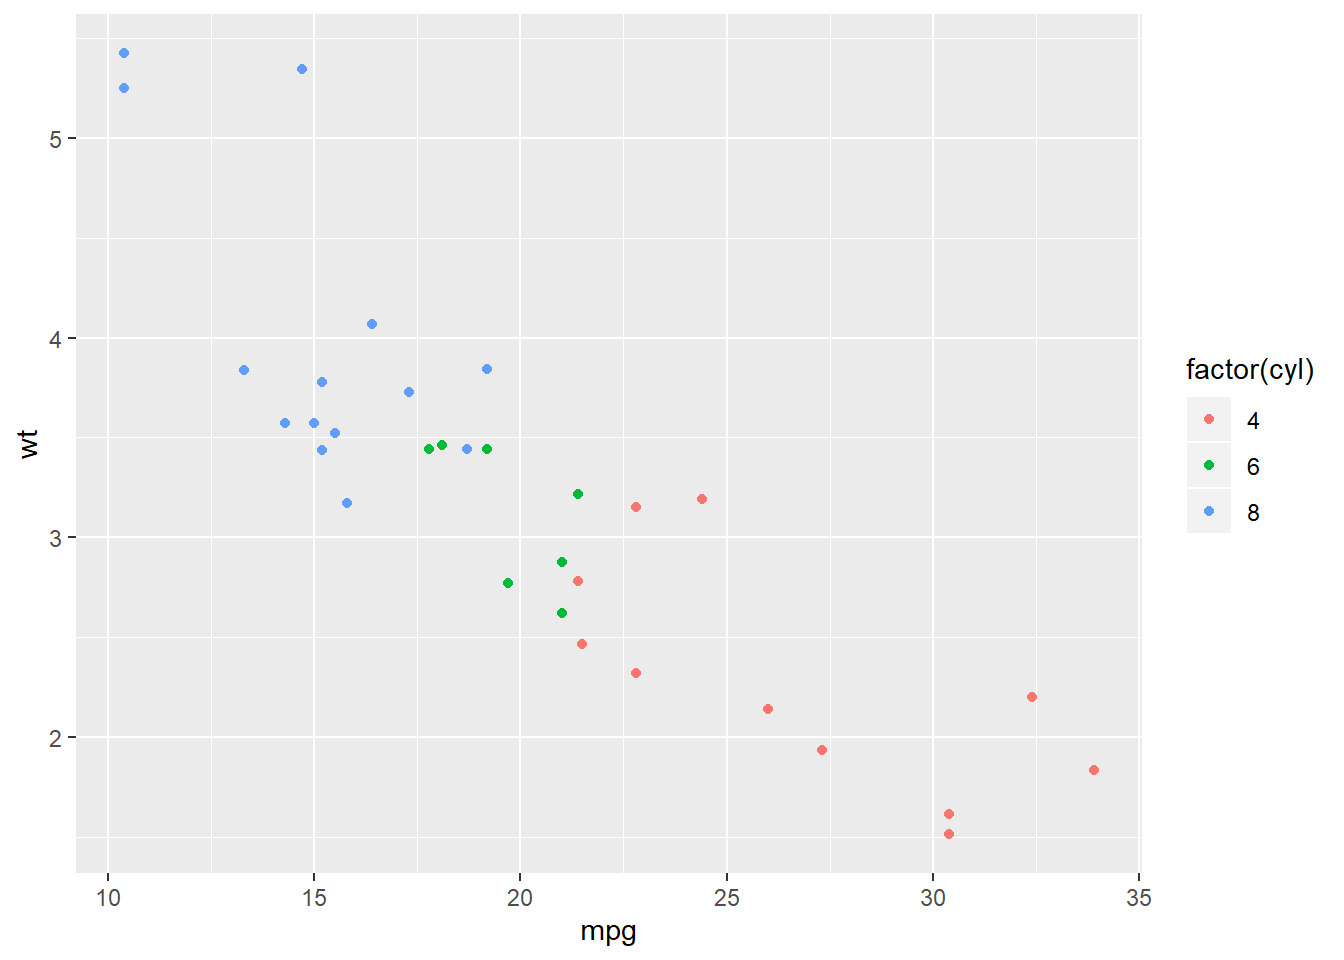
\includegraphics{livro_files/figure-latex/unnamed-chunk-115-1.pdf}

\hypertarget{boxplot}{%
\subsection{Boxplot}\label{boxplot}}

O Boxplot (ou gráfico de caixa) representa graficamente o valor mínimo,
o 1º quartil, a media, o 3º quartil e o valor máximo de uma variável.

Esse é o Boxplot para a variável \emph{Petal.Width}:

\begin{Shaded}
\begin{Highlighting}[]
\KeywordTok{boxplot}\NormalTok{(iris}\OperatorTok{$}\NormalTok{Petal.Width)}
\end{Highlighting}
\end{Shaded}

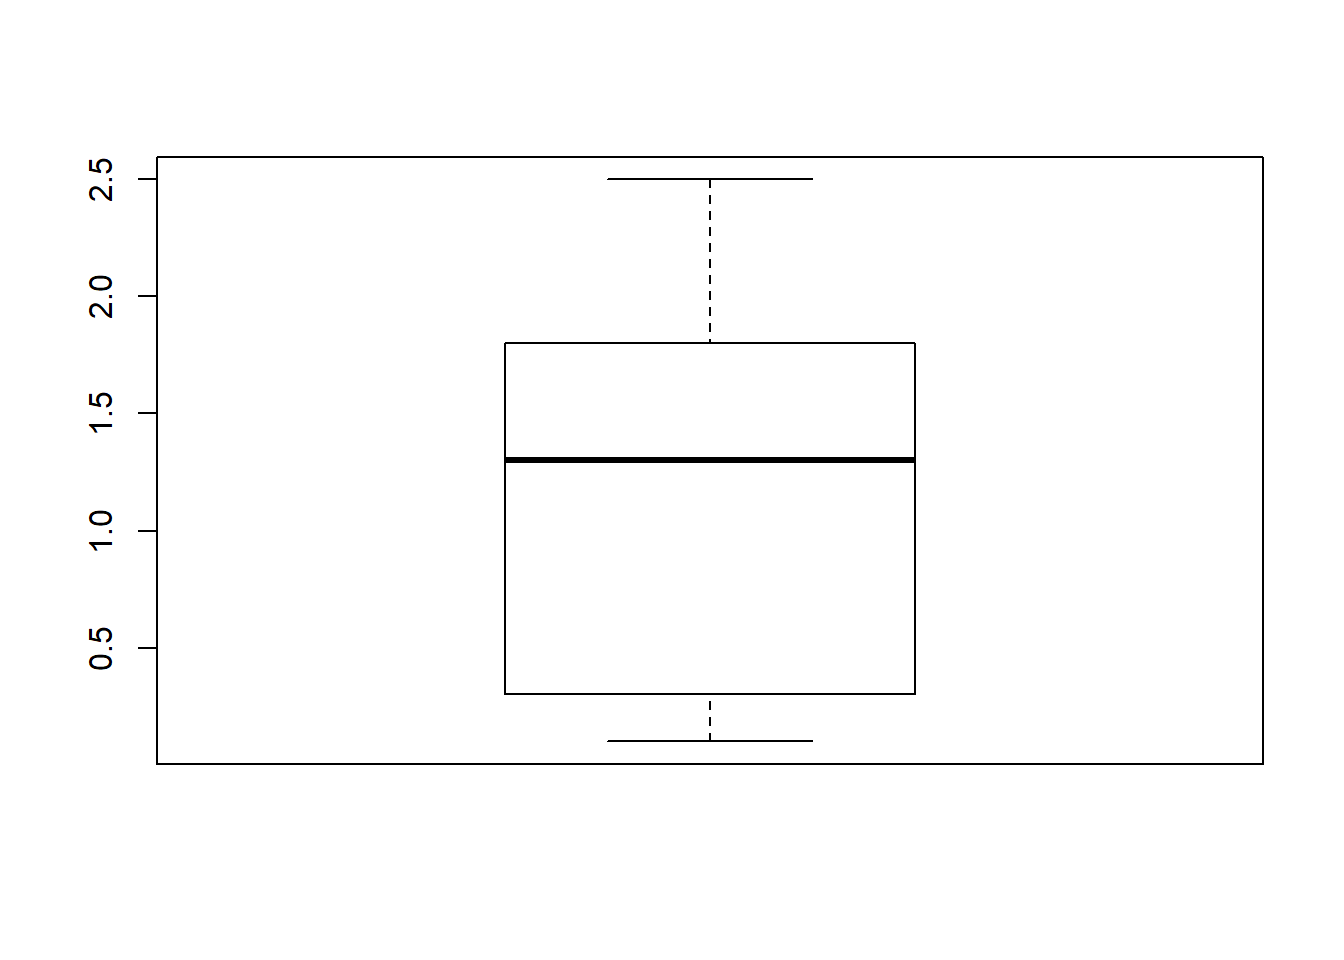
\includegraphics{livro_files/figure-latex/unnamed-chunk-116-1.pdf}

www.luisotavio.pro

\hypertarget{criando-gruxe1ficos-no-r}{%
\chapter{Criando Gráficos no R}\label{criando-gruxe1ficos-no-r}}

A comunicação dos resultados talvez seja a parte mais importante do
trabalho de um cientista de dados. Digo isso porque sem apresentar seus
resultados de forma eficiente e clara, todo o trabalho desenvolvido é
inútil.

A visualização de dados, representada por gráficos, é praticamente
indispensável em qualquer apresentação de um projeto desenvolvido por um
Cientista de Dados.

Certamente as cores e os tamanhos das barras, colunas ou qualquer outra
representação vão facilitar muito o entendimento da mensagem que você
deseja apresentar.

E posso te garantir que somos extremamente bem servidos quando o assunto
é visualização de dados com a linguagem R.

Existe uma grande quantidade de bibliotecas que podemos usar para fazer
gráficos realmente muito bonitos, claros e que irão surpreender os
leitores de seus relatórios ou \emph{dashboards}.

Não é o objetivo desse e-book falar sobre todas essas bibliotecas, mas
vou citar aqui as minhas favoritas:

\begin{itemize}
\tightlist
\item
  ggplot2
\item
  plot.ly
\item
  googleVis
\item
  rCharts
\item
  leaflet
\end{itemize}

Dentre as 5 possibilidades aqui citadas, destaco a primeira:
\texttt{ggplot2}. Iremos aprofundar mais nessa biblioteca pela
quantidade de possibilidades que ela nos traz.

Usando a biblioteca \texttt{ggplot2} você irá conseguir fazer
praticamente todos os tipos de gráficos disponíveis e com enorme
capacidade de customização do seu gráfico.

A medida que você for dominando a linguagem R, sugiro que também explore
outras bibliotecas. Muitas vezes as bibliotecas \texttt{plot.ly},
\texttt{googleVis} e \texttt{rCharts} irão te possibilitar a criação de
gráficos mais chamativos do que a biblioteca \texttt{ggplot2}.

Eu costumo escolher a biblioteca que irei usar de acordo com o gráfico
que desejo fazer.

A biblioteca \texttt{leaflet}, por exemplo, é específica para a
construção de \textbf{mapas} interativos.

\hypertarget{criando-gruxe1ficos-com-a-biblioteca-ggplot2}{%
\section{\texorpdfstring{Criando gráficos com a biblioteca
\emph{ggplot2}}{Criando gráficos com a biblioteca ggplot2}}\label{criando-gruxe1ficos-com-a-biblioteca-ggplot2}}

Os gráficos da biblioteca partem de uma ideia bem simples:

Todos os gráficos podem ser construídos com 3 elementos:

\begin{itemize}
\tightlist
\item
  O conjunto de dados
\item
  Um sistema de coordenadas
\item
  As marcas de representação visual (linhas, colunas, pontos, etc)
\end{itemize}

Na prática, veremos como podemos criar um gráfico simples e depois ir
aperfeiçoando e personalizando de acordo com a nossa necessidade. Esse
aperfeiçoamento acontece com novas linhas de código, que são
acrescentadas ao gráfico que já foi criado.

Instalando o pacote \texttt{ggplot2}:

\begin{Shaded}
\begin{Highlighting}[]
\KeywordTok{install.packages}\NormalTok{(}\StringTok{"ggplot2"}\NormalTok{)}
\end{Highlighting}
\end{Shaded}

\hypertarget{seu-primeiro-gruxe1fico}{%
\subsection{Seu primeiro gráfico}\label{seu-primeiro-gruxe1fico}}

O código a seguir é dividido com os 3 elementos que citamos acima. O
primeiro elemento é o \textbf{conjunto de dados} \texttt{mtcars}.
\emph{Dataset} que contém informações de diferentes modelos de carros.

O segundo elemento está dentro da função \texttt{aes()}, que é usada
para definir a estética do gráfico (abreviação para \emph{aesthetics} -
estética em inglês).

Nesse elemento, definimos os \textbf{eixos do gráfico}. O gráfico irá
mostrar a relação entre duas variáveis. A variável \emph{mpg} (miles per
gallon - Milhas percorridas para 1 galão de combustível) e \emph{wt}
(Weight - peso do carro).

A variável \emph{mpg} será alocada no eixo x (horizontal) e a variável
\emph{wt} no eixo y (vertical).

O terceiro elemento são as \textbf{marcas de representação visual do
gráfico} e são definidos pela função \texttt{geom\_point()}.

Como nesse exemplo não há nenhuma customização, a função
\texttt{geom\_point()} será vazia.

\begin{Shaded}
\begin{Highlighting}[]
\KeywordTok{library}\NormalTok{(ggplot2)}

\KeywordTok{ggplot}\NormalTok{(mtcars, }\KeywordTok{aes}\NormalTok{(mpg, wt)) }\OperatorTok{+}
\StringTok{  }\KeywordTok{geom_point}\NormalTok{()}
\end{Highlighting}
\end{Shaded}

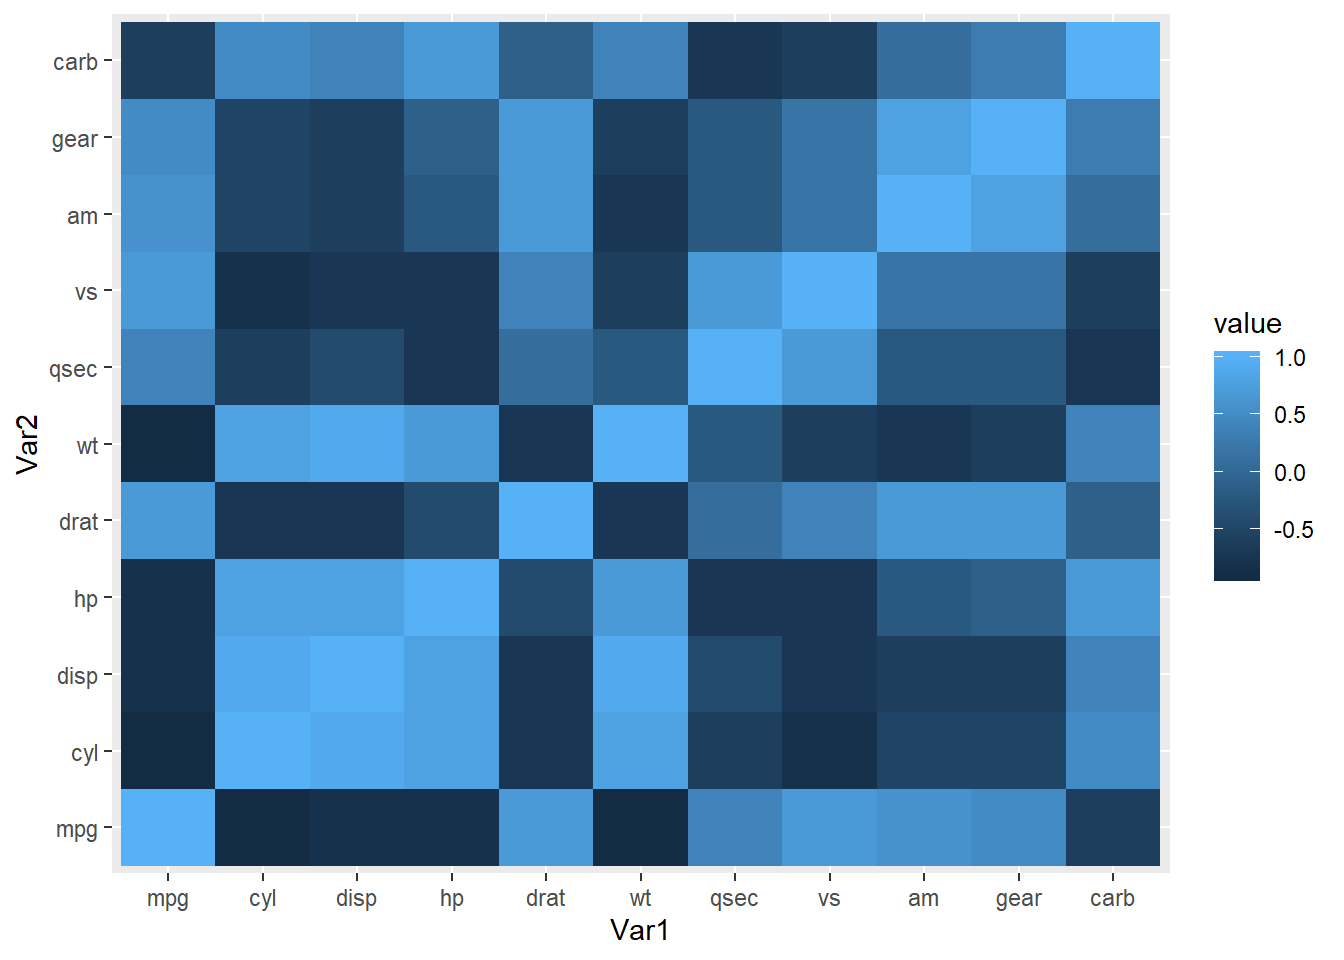
\includegraphics{livro_files/figure-latex/unnamed-chunk-119-1.pdf}

\hypertarget{incrementando-o-gruxe1fico}{%
\subsection{Incrementando o gráfico}\label{incrementando-o-gruxe1fico}}

Podemos incrementar um pouco o nosso gráfico adicionando uma terceira
variável. Vamos adicionar a variável \emph{cyl}, que representa o número
de cilindros do carro.

Agora, com 3 variáveis, o gráfico continuará sendo bi-dimensional.
Porém, os pontos do gráfico serão coloridos de acordo com a variável
\emph{cyl}.

Antes de criarmos o gráfico, segue uma consideração: a variável
\emph{cyl} está classificada como numérica.

\begin{Shaded}
\begin{Highlighting}[]
\KeywordTok{class}\NormalTok{(mtcars}\OperatorTok{$}\NormalTok{cyl)}
\end{Highlighting}
\end{Shaded}

\begin{verbatim}
## [1] "numeric"
\end{verbatim}

Os carros desse \emph{dataset} possuem 4, 6 ou 8 cilindros. Então, nesse
caso será mais interessante tratar a variável \emph{cyl} como
categórica. Essa pequena alteração fará muita diferença na visualização
dos dados, pois irá colorir cada uma das categorias com cores totalmente
distintas.

Caso se considerasse a variável \emph{cyl} como numérica, as cores de
cada quantidade de cilindros sofreriam alterações apenas no tom da cor,
dificultando a visualização de cada um dos grupos.

Para tratar a variável \emph{cyl} como categórica, vamos apenas
adicionar a função \texttt{factor()} ao inserir a variável na criação do
gráfico.

\begin{Shaded}
\begin{Highlighting}[]
\KeywordTok{library}\NormalTok{(ggplot2)}

\KeywordTok{ggplot}\NormalTok{(mtcars, }\KeywordTok{aes}\NormalTok{(mpg, wt,}\DataTypeTok{color=}\KeywordTok{factor}\NormalTok{(cyl))) }\OperatorTok{+}
\StringTok{  }\KeywordTok{geom_point}\NormalTok{()}
\end{Highlighting}
\end{Shaded}

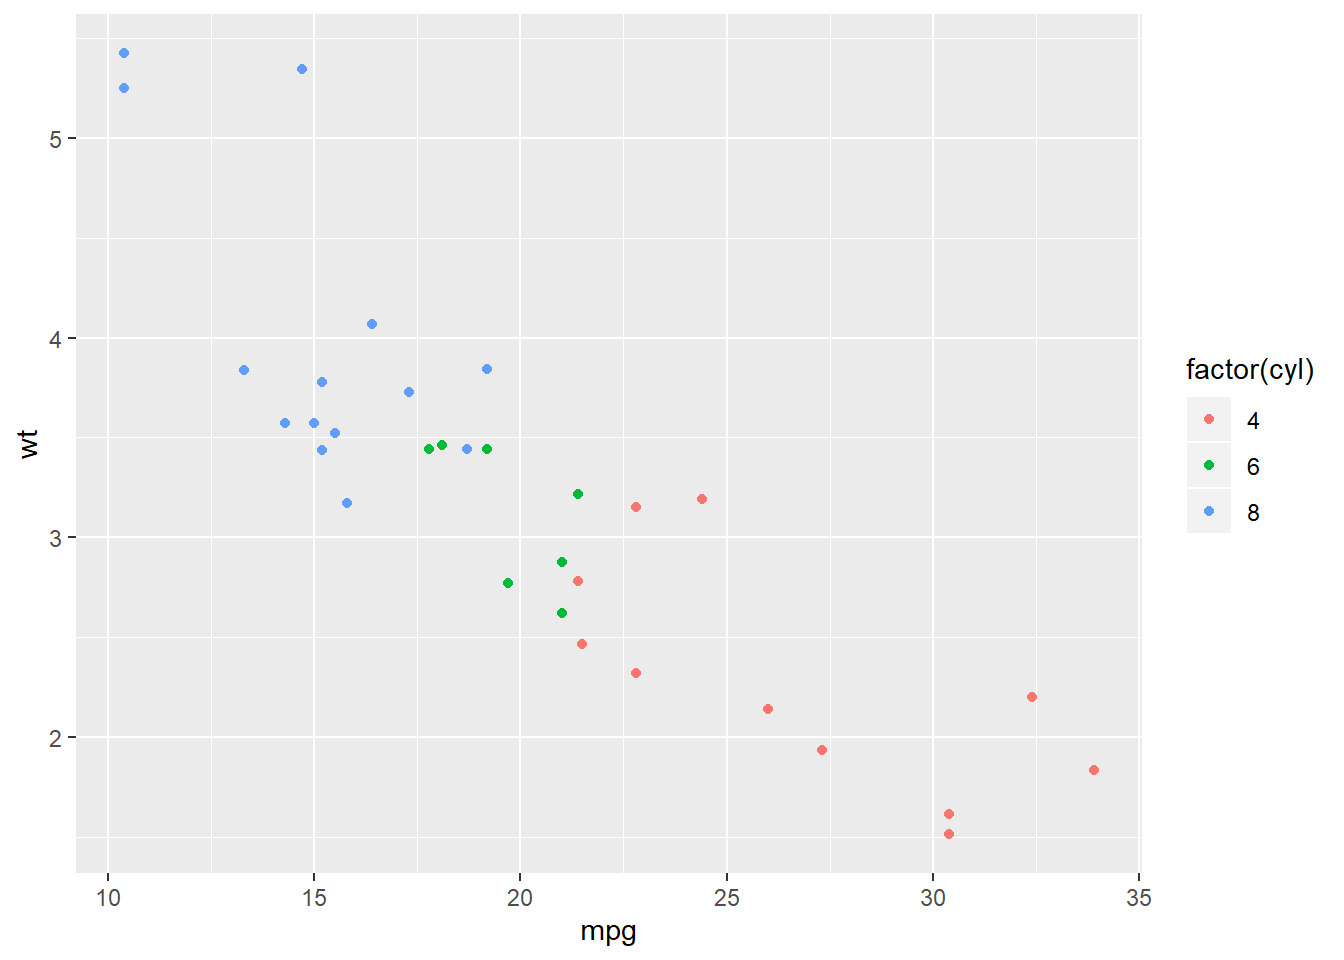
\includegraphics{livro_files/figure-latex/unnamed-chunk-121-1.pdf}

Então, nesse último colocamos duas variáveis nos tradicionais eixos x e
y - \emph{mpg} e \emph{wt}, respectivamente. Além disso, colorimos os
pontos do gráfico de acordo com a quantidade de cilindros de cada carro.

E se precisássemos adicionar mais informações a esse gráfico?

\hypertarget{o-gruxe1fico-de-bolhas---bubble-chart}{%
\subsection{O Gráfico de Bolhas - Bubble
Chart}\label{o-gruxe1fico-de-bolhas---bubble-chart}}

Além dessas 3 variáveis, se usarmos o gráfico de bolhas, poderemos
adicionar uma 4ª variável ao nosso gráfico sem comprometer a sua
qualidade.

Então, a variável \emph{mpg} será representada pelo eixo x, a variável
\emph{wt} pelo eixo y, a quantidade de cilindros será destacada por
cores diferentes de cada bolha.

A quarta variável escolhida é a \emph{qsec}, que mede quantos segundos o
carro precisa para alcançar 0,25 milhas.

Em nosso gráfico, a variável \emph{qsec} será representada pelo tamanho
da bolha.

Cada bolha é um ponto do gráfico e representa um carro do conjunto de
dados.

\begin{Shaded}
\begin{Highlighting}[]
\KeywordTok{ggplot}\NormalTok{(mtcars, }\KeywordTok{aes}\NormalTok{(mpg, wt))}\OperatorTok{+}\StringTok{ }\CommentTok{#definição de qual é o dataset e quais são as variáveis dos eixos x e y.}
\StringTok{  }\KeywordTok{geom_point}\NormalTok{(}\KeywordTok{aes}\NormalTok{(}\DataTypeTok{color =} \KeywordTok{factor}\NormalTok{(cyl), }\DataTypeTok{size =}\NormalTok{ qsec), }\DataTypeTok{alpha =} \FloatTok{0.5}\NormalTok{) }\OperatorTok{+}\StringTok{ }\CommentTok{#definição de qual variável será representada pela cor e qual será representada pelo tamanho das bolhas.}
\StringTok{  }\KeywordTok{scale_color_manual}\NormalTok{(}\DataTypeTok{values =} \KeywordTok{c}\NormalTok{(}\StringTok{"#00AFBB"}\NormalTok{, }\StringTok{"#E7B800"}\NormalTok{, }\StringTok{"#FC4E07"}\NormalTok{)) }\OperatorTok{+}\StringTok{ }\CommentTok{#definição das cores das bolhas.}
\StringTok{  }\KeywordTok{scale_size}\NormalTok{(}\DataTypeTok{range =} \KeywordTok{c}\NormalTok{(}\FloatTok{0.5}\NormalTok{, }\DecValTok{12}\NormalTok{))  }\CommentTok{# Amplitude do tamanho das bolhas}
\end{Highlighting}
\end{Shaded}

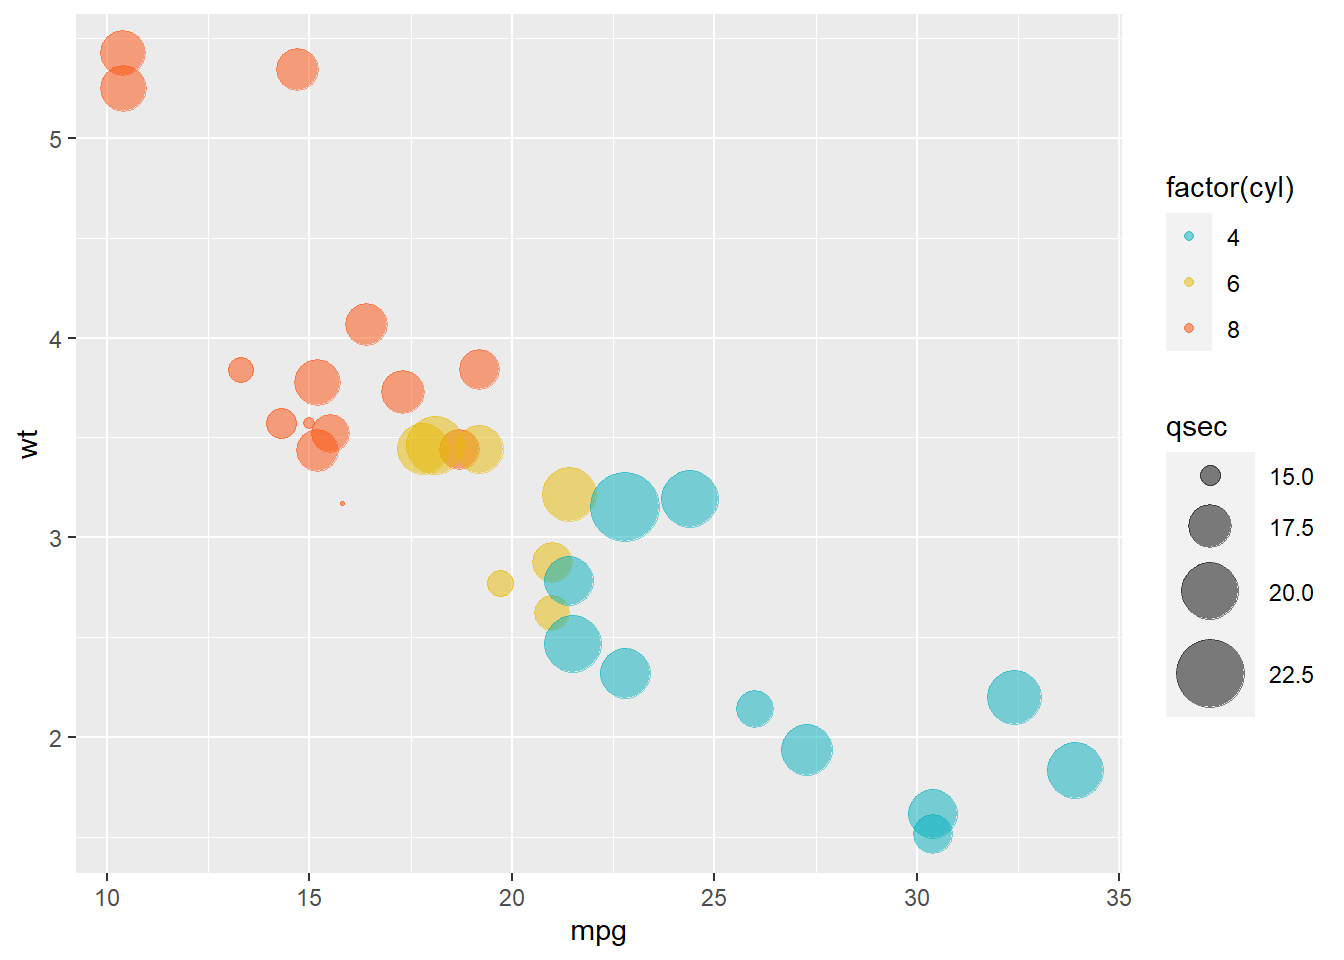
\includegraphics{livro_files/figure-latex/unnamed-chunk-122-1.pdf}

Pelos dois últimos gráficos, há fortes indícios que quanto maior o peso
do carro (\emph{wt}), menor é a quantidade de milhas que ele consegue
percorrer com um galão de combustível.

Além disso, parece haver uma relação entre a quantidade de cilindros e
essas duas variáveis. Por exemplo, os carros com 4 cilindros parecem ser
mais leves e rodar mais milhas com um galão de combustível.

\hypertarget{o-gruxe1fico-de-correlauxe7uxe3o}{%
\subsection{O gráfico de
correlação}\label{o-gruxe1fico-de-correlauxe7uxe3o}}

Para verificar a correlação entre as variáveis, podemos simplesmente uma
tabela com a correlação entre elas:

\begin{Shaded}
\begin{Highlighting}[]
\NormalTok{tabela_correlacao <-}\StringTok{ }\KeywordTok{round}\NormalTok{(stats}\OperatorTok{::}\KeywordTok{cor}\NormalTok{(mtcars), }\DecValTok{1}\NormalTok{) }\CommentTok{#a função round é usada para arredondar as casas decimais do resultado.}
\NormalTok{tabela_correlacao}
\end{Highlighting}
\end{Shaded}

\begin{verbatim}
##       mpg  cyl disp   hp drat   wt qsec   vs   am gear carb
## mpg   1.0 -0.9 -0.8 -0.8  0.7 -0.9  0.4  0.7  0.6  0.5 -0.6
## cyl  -0.9  1.0  0.9  0.8 -0.7  0.8 -0.6 -0.8 -0.5 -0.5  0.5
## disp -0.8  0.9  1.0  0.8 -0.7  0.9 -0.4 -0.7 -0.6 -0.6  0.4
## hp   -0.8  0.8  0.8  1.0 -0.4  0.7 -0.7 -0.7 -0.2 -0.1  0.7
## drat  0.7 -0.7 -0.7 -0.4  1.0 -0.7  0.1  0.4  0.7  0.7 -0.1
## wt   -0.9  0.8  0.9  0.7 -0.7  1.0 -0.2 -0.6 -0.7 -0.6  0.4
## qsec  0.4 -0.6 -0.4 -0.7  0.1 -0.2  1.0  0.7 -0.2 -0.2 -0.7
## vs    0.7 -0.8 -0.7 -0.7  0.4 -0.6  0.7  1.0  0.2  0.2 -0.6
## am    0.6 -0.5 -0.6 -0.2  0.7 -0.7 -0.2  0.2  1.0  0.8  0.1
## gear  0.5 -0.5 -0.6 -0.1  0.7 -0.6 -0.2  0.2  0.8  1.0  0.3
## carb -0.6  0.5  0.4  0.7 -0.1  0.4 -0.7 -0.6  0.1  0.3  1.0
\end{verbatim}

A tabela acima é muito informativa, porém, caso seja visualizada como um
gráfico será muito mais fácil de compreendê-la.

Para criar um gráfico com a correlação entre as variáveis, precisaremos
fazer uma pequena transformação na tabela acima.

A matriz será transformada em uma nova tabela com 3 colunas: duas
colunas com os nomes das variáveis e a terceira coluna com o valor
correspondente da correlação entre elas.

Para isso, usaremos a biblioteca \texttt{reshape2} e a função
\texttt{melt}:

\begin{Shaded}
\begin{Highlighting}[]
\CommentTok{# install.packages("reshape2")  #caso vc não já tenha instalado a biblioteca reshape2, precisa executar essa linha.}
\KeywordTok{library}\NormalTok{(reshape2)}
\NormalTok{melted_tabela_correlacao <-}\StringTok{ }\KeywordTok{melt}\NormalTok{(tabela_correlacao)}
\KeywordTok{head}\NormalTok{(melted_tabela_correlacao)}
\end{Highlighting}
\end{Shaded}

\begin{verbatim}
##   Var1 Var2 value
## 1  mpg  mpg   1.0
## 2  cyl  mpg  -0.9
## 3 disp  mpg  -0.8
## 4   hp  mpg  -0.8
## 5 drat  mpg   0.7
## 6   wt  mpg  -0.9
\end{verbatim}

\begin{Shaded}
\begin{Highlighting}[]
\KeywordTok{library}\NormalTok{(ggplot2)}
\KeywordTok{ggplot}\NormalTok{(}\DataTypeTok{data =}\NormalTok{ melted_tabela_correlacao, }\KeywordTok{aes}\NormalTok{(}\DataTypeTok{x=}\NormalTok{Var1, }\DataTypeTok{y=}\NormalTok{Var2, }\DataTypeTok{fill=}\NormalTok{value)) }\OperatorTok{+}\StringTok{ }
\StringTok{  }\KeywordTok{geom_tile}\NormalTok{()}
\end{Highlighting}
\end{Shaded}

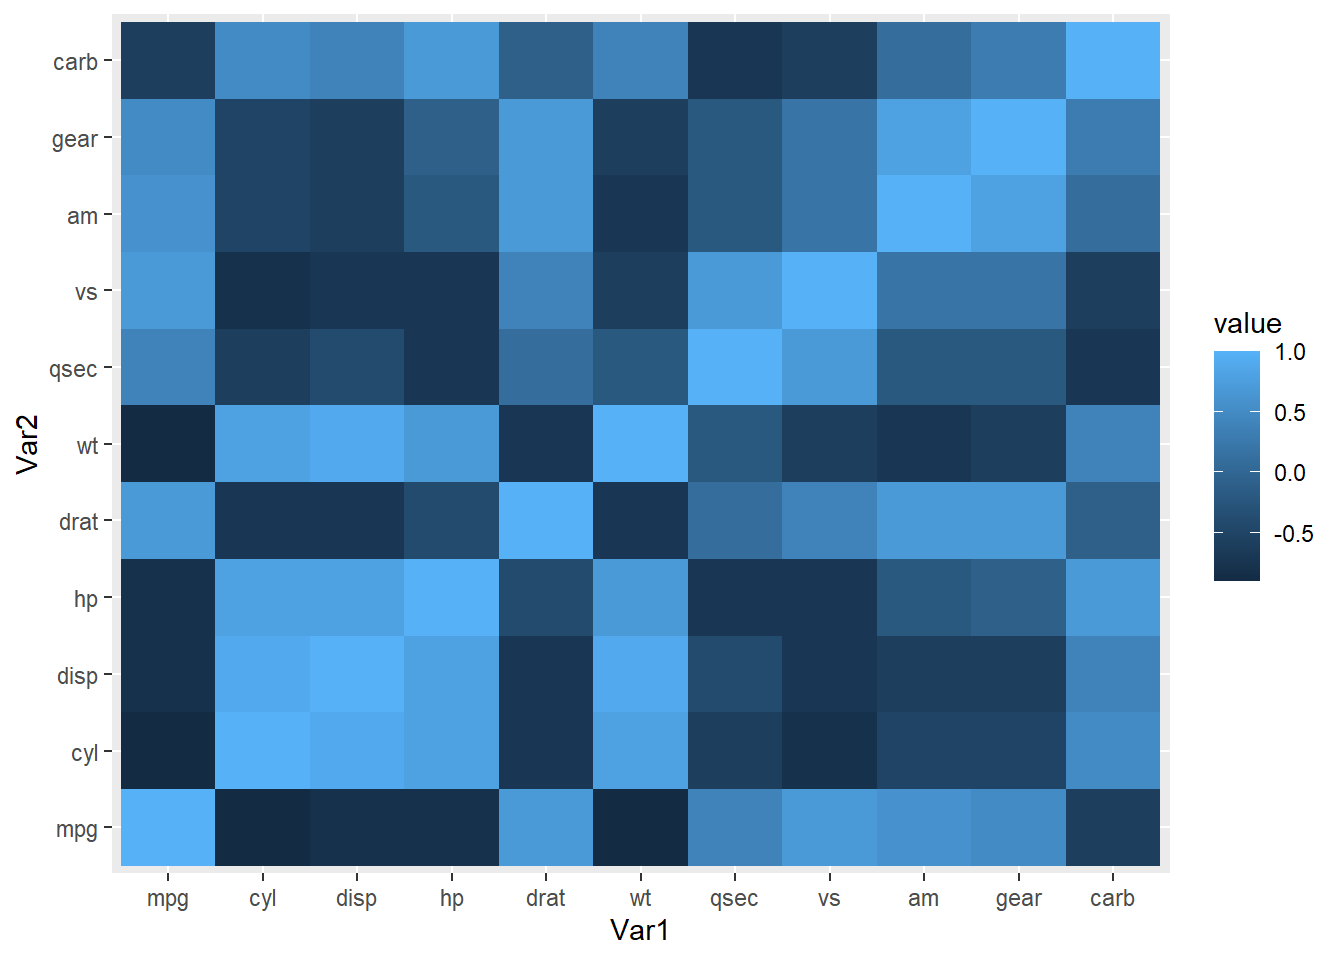
\includegraphics{livro_files/figure-latex/unnamed-chunk-126-1.pdf}

\hypertarget{aperfeiuxe7oando-o-gruxe1fico}{%
\subsection{Aperfeiçoando o
gráfico}\label{aperfeiuxe7oando-o-gruxe1fico}}

Os gráficos facilitam muito a visualização dos dados. Porém, com mais um
pouco de esforço, podemos melhorar muito a visualização desses dados.

\begin{Shaded}
\begin{Highlighting}[]
\NormalTok{tabela_correlacao[}\KeywordTok{lower.tri}\NormalTok{(tabela_correlacao,}\DataTypeTok{diag =}\NormalTok{ T)]<-}\StringTok{ }\OtherTok{NA} \CommentTok{## selecionar apenas a parte superior da matriz (evitando informações repetidas)}
\KeywordTok{head}\NormalTok{(tabela_correlacao)}
\end{Highlighting}
\end{Shaded}

\begin{verbatim}
##      mpg  cyl disp   hp drat   wt qsec   vs   am gear carb
## mpg   NA -0.9 -0.8 -0.8  0.7 -0.9  0.4  0.7  0.6  0.5 -0.6
## cyl   NA   NA  0.9  0.8 -0.7  0.8 -0.6 -0.8 -0.5 -0.5  0.5
## disp  NA   NA   NA  0.8 -0.7  0.9 -0.4 -0.7 -0.6 -0.6  0.4
## hp    NA   NA   NA   NA -0.4  0.7 -0.7 -0.7 -0.2 -0.1  0.7
## drat  NA   NA   NA   NA   NA -0.7  0.1  0.4  0.7  0.7 -0.1
## wt    NA   NA   NA   NA   NA   NA -0.2 -0.6 -0.7 -0.6  0.4
\end{verbatim}

\begin{Shaded}
\begin{Highlighting}[]
\KeywordTok{library}\NormalTok{(reshape2)}
\NormalTok{dados_correlacao <-}\StringTok{ }\KeywordTok{melt}\NormalTok{(tabela_correlacao,}\DataTypeTok{na.rm =}\NormalTok{ T) }\CommentTok{#transformando os dados para as 3 colunas como anteriormente.}
\KeywordTok{head}\NormalTok{(dados_correlacao)}
\end{Highlighting}
\end{Shaded}

\begin{verbatim}
##    Var1 Var2 value
## 12  mpg  cyl  -0.9
## 23  mpg disp  -0.8
## 24  cyl disp   0.9
## 34  mpg   hp  -0.8
## 35  cyl   hp   0.8
## 36 disp   hp   0.8
\end{verbatim}

\begin{Shaded}
\begin{Highlighting}[]
\KeywordTok{library}\NormalTok{(ggplot2)}
\KeywordTok{ggplot}\NormalTok{(}\DataTypeTok{data =}\NormalTok{ dados_correlacao, }\KeywordTok{aes}\NormalTok{(Var2, Var1, }\DataTypeTok{fill =}\NormalTok{ value))}\OperatorTok{+}\StringTok{ }\CommentTok{#seleciona os dados e as variáveis para cada eixo, assim como a variável que determina a cor (value).}
\StringTok{ }\KeywordTok{geom_tile}\NormalTok{(}\DataTypeTok{color =} \StringTok{"white"}\NormalTok{)}\OperatorTok{+}\StringTok{    }\CommentTok{#definindo a cor do contorno de cada quadrado.}
\StringTok{ }\KeywordTok{scale_fill_gradient2}\NormalTok{(}\DataTypeTok{low =} \StringTok{"blue"}\NormalTok{, }\DataTypeTok{high =} \StringTok{"red"}\NormalTok{, }\DataTypeTok{mid =} \StringTok{"white"}\NormalTok{, }\CommentTok{#definindo a escala de cor das correlações}
   \DataTypeTok{midpoint =} \DecValTok{0}\NormalTok{, }\DataTypeTok{limit =} \KeywordTok{c}\NormalTok{(}\OperatorTok{-}\DecValTok{1}\NormalTok{,}\DecValTok{1}\NormalTok{), }\DataTypeTok{space =} \StringTok{"Lab"}\NormalTok{, }\CommentTok{#definindo a escala das correlações}
   \DataTypeTok{name=}\StringTok{"Coef. Correlação"}\NormalTok{) }\OperatorTok{+}\StringTok{ }\CommentTok{#definindo o nome da legenda.}
\StringTok{  }\KeywordTok{theme_minimal}\NormalTok{()}\OperatorTok{+}\StringTok{ }\CommentTok{#tema de fundo do gráfico}
\StringTok{   }\KeywordTok{coord_fixed}\NormalTok{() }\OperatorTok{+}\StringTok{ }\CommentTok{#mantém as coordenadas e as mediadas dos quadrados fixos.}
\StringTok{  }\KeywordTok{labs}\NormalTok{(}\DataTypeTok{x =} \StringTok{"nome eixo x"}\NormalTok{, }\DataTypeTok{y =} \StringTok{"nome eixo y"}\NormalTok{) }\CommentTok{#define o nome para o eixo x e para o eixo y}
\end{Highlighting}
\end{Shaded}

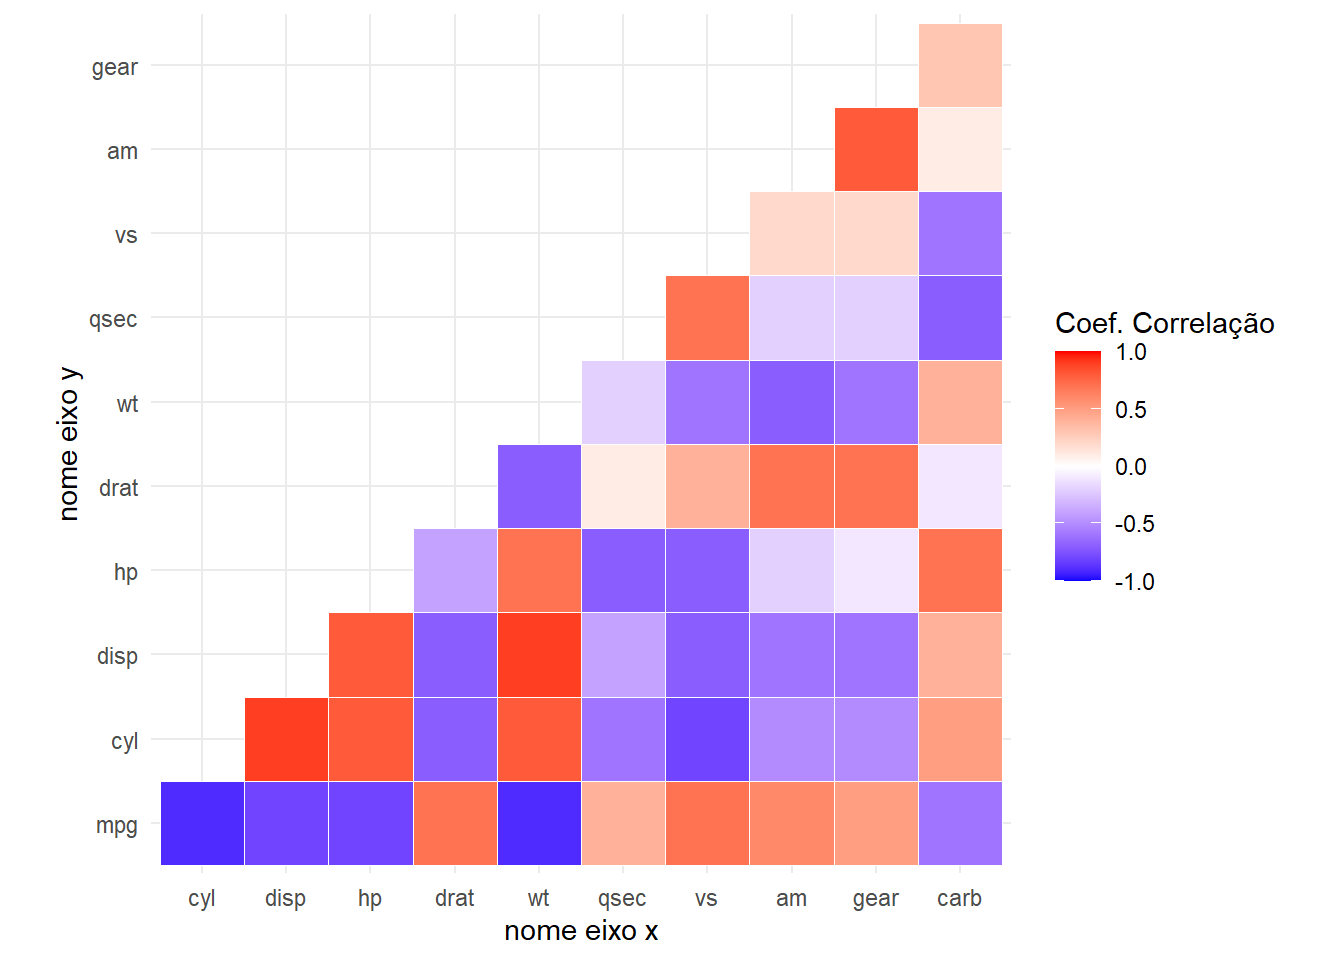
\includegraphics{livro_files/figure-latex/unnamed-chunk-128-1.pdf}

Fique tranquilo que você não precisa decorar as funções acima. É
importante que você leia e entenda o que cada uma está fazendo, só isso.
E isso vai acontecer aos poucos, com a prática.

Digo que você não precisa decorar porque são infinitas possibilidades e
não faz sentido nenhum gastar energia decorando isso. Basta que você
pesquise no Google sobre o gráfico que deseja fazer e escolha o melhor
para o seu caso.

Após encontrar na internet um código do gráfico que você deseja criar,
basta fazer algumas adaptações para o seu caso.

\textbf{Entendendo os comandos do gráfico acima:} assim como nos outros
gráficos do pacote \texttt{ggplot2}, temos o padrão de inserir os dados
(\emph{dados\_correlacao}), depois definir as variáveis para os eixos x
e y e o nome da variável que será colorida (\emph{aes(Var2, Var1, fill =
value)}). Os comandos seguintes são as marcas de representação visual e
customizações do gráfico.

As mesmas estruturas acima podem ser utilizadas para todos os gráficos
da biblioteca \texttt{ggplot2}, que possui diversos tipos de gráficos.

www.luisotavio.pro

Vários mercados precisam de notícias em tempo real, imagine só o mercado
de finanças:

\begin{itemize}
\tightlist
\item
  Uma decisão política, um resultado de uma grande empresa ou um
  acidente são fatores que geram um impacto enorme no mercado
  financeiro.
\end{itemize}

Isso faz que todos os envolvidos fiquem ligados o tempo inteiro em
notícias.

Hoje em dia, na grande parte das vezes ficamos sabendo de notícias pelas
nossas redes sociais. Isso porque as notícias mais relevantes são
postadas e compartilhadas com muita velocidade.

O que também propicia essa velocidade é a informalidade e objetividade
das redes sociais. É muito mais fácil escrever um tweet do que uma
reportagem.

Entre todas as redes sociais, considero que o \textbf{Twitter} seja a
rede social mais voltada para notícias. É uma rede social que está
sempre vivendo a polêmica do momento.

E, no meu trabalho, não é diferente! Usamos muito o Twitter como meio de
informação.

Meu trabalho é diretamente relacionado ao campeonato brasileiro de
futebol e uma das maiores dores dos nossos clientes é justamente não
estar 100\% informado.

Eles precisam saber quem o técnico irá escalar na próxima partida. Essa
informação nunca é divulgada de forma concreta com antecedência.

Então, a nossa principal fonte de notícias é o repórter que trabalha
dentro do clube, que vive o dia a dia dos atletas e acompanha os
treinamentos.

E todas as informações são divulgadas primeiramente no Twitter.

Porém, existem vários repórteres para cada time e, além disso, são
postadas várias informações em seus perfis que não nos interessam.

Então, para resolver esse problema acima, o que eu fiz?

Criei uma lista com 90 repórteres que são destinados a acompanhar o dia
a dia de clubes da Serie A do Campeonato Brasileiro.

Além disso, criei uma plataforma para ler as postagens e decidir se ela
é interessante ou não para o fim que desejo.

Nessa plataforma, eu consigo ver o horário da postagem, quem postou,
qual o time que ele acompanha, o texto da postagem, seu engajamento e
também clicar para ir direto ao post.

Poderia ter sido criado um gatilho para definir se o post deveria ser
retuítado ou não, por exemplo:

\begin{itemize}
\item
  Compartilhar os tweets com maior número de curtidas
\item
  Compartilhar os tweets com determinadas palavras-chave
\item
  Compartilhar os tweets com mais compartilhamentos
\end{itemize}

Porém, como é a primeira versão da ferramenta, optei por deixar a opção
de retweet com um gatilho manual. Alguém precisará clicar em no botão
``RETWEET'' para compartilhar o post.

Essa opção é até mais complexa para o nosso desenvolvimento aqui. Porém,
acredito que será mais eficaz para evitar compartilhamentos indesejados.

Para o desenvolvimento da ferramenta, utilizei a integração com a API do
Twitter usando a biblioteca \texttt{rtweet}.

Vou mostrar aqui quais foram as partes chaves no desenvolvimento da
ferramenta:

\hypertarget{passo-1---acesso-a-api-do-twitter}{%
\subsection{PASSO 1 - ACESSO A API DO
TWITTER}\label{passo-1---acesso-a-api-do-twitter}}

O tem uma ferramenta para facilitar a busca das informações que fazemos
na plataforma deles, o que torna a tarefa mais fácil e rápida.

Caso você queira criar a sua própria busca, praticando no seu
computador, terá que se cadastrar no Twitter como um desenvolvedor. É
bem fácil e leva poucos minutos.

Aqui nesse endereço você tem todas as instruções:
\url{https://cran.r-project.org/web/packages/rtweet/vignettes/auth.html}

\begin{Shaded}
\begin{Highlighting}[]
\KeywordTok{library}\NormalTok{(rtweet)}
\CommentTok{#substitua os 4 valores seguintes pelos valores correspondentes ao seu login}

\CommentTok{# api_key <- "XXXXXXXXX"}
\CommentTok{# api_secret_key <- "XXXXXXXXX"}
\CommentTok{# access_token <- "XXXXXXXXX"}
\CommentTok{# access_token_secret <- "XXXXXXXXX"}

\CommentTok{## authenticate via web browser}
\NormalTok{token <-}\StringTok{ }\KeywordTok{create_token}\NormalTok{(}
  \DataTypeTok{app =} \StringTok{"nome do seu app"}\NormalTok{, }\CommentTok{#substituir}
  \DataTypeTok{consumer_key =}\NormalTok{ api_key,}
  \DataTypeTok{consumer_secret =}\NormalTok{ api_secret_key,}
  \DataTypeTok{access_token =}\NormalTok{ access_token,}
  \DataTypeTok{access_secret =}\NormalTok{ access_token_secret)}
\end{Highlighting}
\end{Shaded}

\hypertarget{passo-2---buscar-os-tweets-de-cada-repuxf3rter}{%
\subsection{PASSO 2 - BUSCAR OS TWEETS DE CADA
REPÓRTER}\label{passo-2---buscar-os-tweets-de-cada-repuxf3rter}}

O \textbf{nome de usuário} de cada repórter está na tabela
\texttt{setorista} na coluna \texttt{screen\_name}.

Então eu executo a função \texttt{get\_timeline} para cada repórter e
busco os 15 primeiros tweets.

Além disso, já escolho quais as variáveis eu desejo armazenar em cada
busca, usando a função \texttt{select}.

\begin{Shaded}
\begin{Highlighting}[]
\NormalTok{todos_tweets<-}\KeywordTok{data.frame}\NormalTok{()}
\ControlFlowTok{for}\NormalTok{(set }\ControlFlowTok{in} \DecValTok{1}\OperatorTok{:}\KeywordTok{nrow}\NormalTok{(setoristas))\{}
\NormalTok{  tweets_set <-}\StringTok{ }\KeywordTok{get_timeline}\NormalTok{(setoristas}\OperatorTok{$}\NormalTok{screen_name[set],}\DataTypeTok{n =} \DecValTok{15}\NormalTok{) }\OperatorTok
\StringTok{    }\KeywordTok{select}\NormalTok{(created_at,screen_name,text,favorite_count,status_id,followers_count,media_url)}
\NormalTok{  todos_tweets<-}\KeywordTok{rbind}\NormalTok{(todos_tweets,tweets_set)}
\NormalTok{\}}
\end{Highlighting}
\end{Shaded}

\hypertarget{passo-3---visualizauxe7uxe3o-das-buscas-e-o-retweet}{%
\subsection{PASSO 3 - VISUALIZAÇÃO DAS BUSCAS E O
RETWEET}\label{passo-3---visualizauxe7uxe3o-das-buscas-e-o-retweet}}

Esse é o resultado da ferramenta para escolher as informações que são
úteis e devem ser retuítadas.

\begin{figure}
\centering

\includegraphics[width=1\textwidth,height=\textheight]{/images/post_interno/twitter_guru.png}
\caption{Ferramenta Retweet}
\end{figure}

Houve uma exceção nesse post e a ferramenta construída não foi
disponibilizada na íntegra, pois ela permite que se faça posts no MEU
Twitter.

Espero que entenda e aproveito para falar que caso tenha alguma dúvida
ou precise de ajuda, estou à disposição.

\textbf{Nesse post você vai aprender 5 formas diferentes de como filtrar
os dados da sua tabela no R.}

São várias as razões que você pode precisar filtrar os seus dados em uma
análise de dados:

\begin{itemize}
\tightlist
\item
  Visualizar as 50 primeiras linhas da sua tabela
\item
  Visualizar todos os registros que possuem um determinado valor para a
  variável X
\item
  Excluir todos os registros que tenham a variável Y igual a 2, por
  exemplo\ldots{}
\item
  Ou até mesmo buscar uma amostra aleatória dos seus dados.
\end{itemize}

Porém, alguns métodos são mais adequados que os outros, dependendo do
seu objetivo.

Então, vou falar aqui todas as 5 maneiras e quando usar cada uma delas.

Em nossos exemplos, vou usar o dataset \emph{iris} que já é carregado
automaticamente no R.

\hypertarget{filtro-de-dados-pelas-linhas-e-colunas}{%
\subsection{Filtro de dados pelas linhas e
colunas}\label{filtro-de-dados-pelas-linhas-e-colunas}}

Essa a é a forma mais simples de selecionar dados do seu dataset. E, na
minha opinião, deve ser usada com muita cautela.

O nosso dataset se chama \textbf{iris}, então quando escrevemos o
comando

\begin{Shaded}
\begin{Highlighting}[]
\NormalTok{subset_iris1<-iris[}\DecValTok{1}\OperatorTok{:}\DecValTok{30}\NormalTok{,]}
\end{Highlighting}
\end{Shaded}

estamos selecionando as linhas de 1 a 30 do dataset \textbf{iris}.

Quando abrimos os colchetes depois do dataset, temos dois campos
separados pela vírgula. Informamos quais as linhas que queremos
selecionar antes da vírgula.

Depois da vírgula informamos quais as colunas queremos selecionar. Como
deixei em branco, o R irá retornar todas as colunas do dataset.

Agora, se eu colocar o comando

\begin{Shaded}
\begin{Highlighting}[]
\NormalTok{subset_iris1<-iris[,}\KeywordTok{c}\NormalTok{(}\DecValTok{1}\NormalTok{,}\DecValTok{3}\NormalTok{,}\DecValTok{5}\NormalTok{)]}
\end{Highlighting}
\end{Shaded}

O R irá retornar todas as linhas do dataset \textbf{iris} (pois o campo
antes da vírgula está vazio) e irá selecionar as colunas 1, 3 e 5, pois
essas foram as colunas que eu coloquei no vetor das colunas.

Você também pode combinar os critérios das linhas e colunas ao mesmo
tempo. Desta forma, é possível até escolher até um único elemento
contido na tabela. Por exemplo:

Caso você deseje saber qual o valor da 90ª linha para a coluna 5, o
comando será o seguinte:

\begin{Shaded}
\begin{Highlighting}[]
\NormalTok{subset_iris1<-iris[}\DecValTok{90}\NormalTok{,}\DecValTok{5}\NormalTok{]}
\end{Highlighting}
\end{Shaded}

Mas porque eu disse que o método deve ser usado com cautela?

Porque, como você viu, ele é extremamente manual. Então, será útil caso
você precise pesquisas ou explorações isoladas.

Mas, de forma alguma, recomendo que você use esse método para fazer
alterações no seu banco de dados que precisem ser generalizadas para
todos os dados.

\hypertarget{excluir-dados-pelas-linhas-e-colunas}{%
\subsection{Excluir dados pelas linhas e
colunas}\label{excluir-dados-pelas-linhas-e-colunas}}

Para excluir determinadas linhas ou colunas, vamos usar o mesmo
raciocínio do item anterior.

Vamos colocar o nome do dataset e os colchetes. Dentro dos colchetes
iremos colocar na mesma ordem: primeiro as linhas e depois da vírgula
colocamos as colunas.

Porém, como queremos excluir as linhas/colunas, iremos colocar um sinal
de ``-'' antes dos números.

Por exemplo, se queremos excluir as linhas 10, 11 e 12 do dataset e
excluir a coluna 4, o comando será:

\begin{Shaded}
\begin{Highlighting}[]
\NormalTok{subset_iris2<-iris[}\OperatorTok{-}\NormalTok{(}\DecValTok{10}\OperatorTok{:}\DecValTok{12}\NormalTok{),}\OperatorTok{-}\DecValTok{4}\NormalTok{]}
\end{Highlighting}
\end{Shaded}

E, da mesma forma, se queremos excluir linhas e colunas salteadas,
colocamos os números dentro da função de vetor c().

\begin{Shaded}
\begin{Highlighting}[]
\NormalTok{subset_iris2<-iris[}\OperatorTok{-}\KeywordTok{c}\NormalTok{(}\DecValTok{10}\NormalTok{,}\DecValTok{50}\NormalTok{,}\DecValTok{90}\NormalTok{),}\OperatorTok{-}\KeywordTok{c}\NormalTok{(}\DecValTok{1}\NormalTok{,}\DecValTok{3}\NormalTok{)]}
\end{Highlighting}
\end{Shaded}

Então, o comando acima retornou o dataset \textbf{iris} sem as linhas
10, 50 e 90 e também excluiu as colunas 1 e 3.

\hypertarget{filtro-de-dados-combinando-a-funuxe7uxe3o-which}{%
\subsection{Filtro de dados combinando a função
which()}\label{filtro-de-dados-combinando-a-funuxe7uxe3o-which}}

Esse método, assim como os seguintes, já podem ser usados em grandes
bases de dados de forma segura. Mesmo que você não veja ou conheça todas
as linhas da tabela.

O filtro se aplicará por uma condição que vamos estabelecer.

Antes de aplicar o filtro, vou explicar rapidamente como funciona a
lógica da função \emph{which()}.

A função \emph{which()} irá retornar um vetor com o número das linhas
que atendem a condição que você estabeleceu.

Por exemplo:

\begin{Shaded}
\begin{Highlighting}[]
\KeywordTok{which}\NormalTok{(iris}\OperatorTok{$}\NormalTok{Sepal.Length}\OperatorTok{>}\DecValTok{6}\NormalTok{)}
\end{Highlighting}
\end{Shaded}

\begin{verbatim}
##  [1]  51  52  53  55  57  59  64  66  69  72  73  74  75  76  77  78  87  88  92
## [20]  98 101 103 104 105 106 108 109 110 111 112 113 116 117 118 119 121 123 124
## [39] 125 126 127 128 129 130 131 132 133 134 135 136 137 138 140 141 142 144 145
## [58] 146 147 148 149
\end{verbatim}

O comando acima irá retornar todas as linhas do dataset \emph{iris} que
possuem um valor maior que 6 para a coluna Sepal.Length.

Se o comando irá retornar um vetor com todas as linhas que queremos
escolher, podemos adaptar a função \_which() no 1º método falado aqui e
selecionar as linhas que precisamos.

Ou seja:

\begin{Shaded}
\begin{Highlighting}[]
\NormalTok{subset_iris3<-iris[}\KeywordTok{which}\NormalTok{(iris}\OperatorTok{$}\NormalTok{Sepal.Length}\OperatorTok{>}\DecValTok{6}\NormalTok{),]}
\end{Highlighting}
\end{Shaded}

\hypertarget{filtro-de-dados-usando-a-funuxe7uxe3o-subset}{%
\subsection{Filtro de dados usando a função
subset()}\label{filtro-de-dados-usando-a-funuxe7uxe3o-subset}}

Você vai perceber que a função subset() é bem intuitiva. Ela só precisa
de 3 argumentos.

\begin{itemize}
\item
  O primeiro argumento que você irá colocar na função é o nome do
  dataset.
\item
  Depois, você irá colocar a condição para cada \emph{linha} que será
  filtrada.
\item
  E, por último, quais as colunas que devem permanecer no dataset que
  você está criando.
\end{itemize}

Vamos supor que a gente deseje montar um novo dataset chamado
``setosa''.

Nele, vamos filtrar apenas os registros do dataset \textbf{iris} que
tenham a variável ``Species'' igual a ``setosa''.

Vou escolher também só as 3 primeiras colunas para o meu novo dataset.

\begin{Shaded}
\begin{Highlighting}[]
\NormalTok{setosa_dataset<-}\KeywordTok{subset}\NormalTok{(iris,Species}\OperatorTok{==}\StringTok{"setosa"}\NormalTok{,}\DataTypeTok{select =} \KeywordTok{c}\NormalTok{(}\StringTok{"Sepal.Length"}\NormalTok{,}\StringTok{"Sepal.Width"}\NormalTok{,}\StringTok{"Petal.Length"}\NormalTok{))}
\end{Highlighting}
\end{Shaded}

OU

\begin{Shaded}
\begin{Highlighting}[]
\NormalTok{setosa_dataset<-}\KeywordTok{subset}\NormalTok{(iris,Species}\OperatorTok{==}\StringTok{"setosa"}\NormalTok{,}\DecValTok{1}\OperatorTok{:}\DecValTok{3}\NormalTok{)}
\end{Highlighting}
\end{Shaded}

Caso você não queira excluir nenhuma coluna, não coloque o último
argumento:

\begin{Shaded}
\begin{Highlighting}[]
\NormalTok{setosa_dataset<-}\KeywordTok{subset}\NormalTok{(iris,Species}\OperatorTok{==}\StringTok{"setosa"}\NormalTok{)}
\end{Highlighting}
\end{Shaded}

\hypertarget{filtrar-usando-a-funuxe7uxe3o-filter-e-select}{%
\subsection{Filtrar usando a função filter() e
select()}\label{filtrar-usando-a-funuxe7uxe3o-filter-e-select}}

As funções \emph{filter} e \emph{select} fazem parte da biblioteca
\textbf{dplyr}.

Esse pacote é essencial para manipulação de dados. Então, se você ainda
tem ele no R, baixe agora mesmo usando o comando:

\begin{Shaded}
\begin{Highlighting}[]
\KeywordTok{install.packages}\NormalTok{(}\StringTok{"dplyr"}\NormalTok{)}
\end{Highlighting}
\end{Shaded}

Para carregar o pacote, você precisar rodar o comando
\texttt{library(dplyr)}

\textbf{É importante saber que você irá usar o comando ``filter'' para
filtrar as LINHAS e o comando ``select'' para selecionar as COLUNAS.}

\begin{itemize}
\tightlist
\item
  Função filter()
\end{itemize}

Você precisa informar duas coisas para a função: -\textgreater{} Quais
os dados você deseja usar (sua tabela) -\textgreater{} Quais as
condições para filtrar os dados

Vamos filtrar aqui novamente de acordo com a variável ``Species'' do
dataset iris.

Agora vou filtrar todos os registros da espécie ``virginica''.

\begin{Shaded}
\begin{Highlighting}[]
\KeywordTok{library}\NormalTok{(dplyr)}
\NormalTok{virginica_dataset<-}\KeywordTok{filter}\NormalTok{(iris,Species}\OperatorTok{==}\StringTok{"virginica"}\NormalTok{)}
\end{Highlighting}
\end{Shaded}

Bem simples! Mas e se a gente quiser combinar mais de uma condição?

Nesse caso, podemos usar dois \textbf{operadores lógicos} para combinar
as condições: E e OU.

Caso a gente precise que as duas condições aconteçam ao mesmo tempo,
usaremos a condição E (representada pelo \&)

Caso a gente precise que aconteça uma condição OU a outra, usaremos a
condição OU (representada pelo \textbar) - nesse caso, só excluiremos
caso não aconteça nenhuma das duas condições.

Vamos supor que precisamos filtrar os registros da espécie
``versicolor'' \textbf{e} que tenham a variável ``Sepal.Length'' maior
que 6.

\begin{Shaded}
\begin{Highlighting}[]
\KeywordTok{library}\NormalTok{(dplyr)}
\NormalTok{versicolor_dataset<-}\KeywordTok{filter}\NormalTok{(iris,Species}\OperatorTok{==}\StringTok{"versicolor"} \OperatorTok{&}\StringTok{ }\NormalTok{Sepal.Length}\OperatorTok{>}\DecValTok{6}\NormalTok{)}
\end{Highlighting}
\end{Shaded}

\begin{itemize}
\tightlist
\item
  Função select()
\end{itemize}

A função select é muito útil para escolher quais as colunas iremos
manter em nosso dataset.

Assim como a função filter(), ela só precisa de dois argumentos.

O primeiro argumento também será o dataset que você irá selecionar as
colunas.

O segundo argumento é a coluna que deseja selecionar. Claro que você
pode querer selecionar várias colunas, não tem problema. Veja só:

Vamos selecionar as colunas Sepal.Length e Species do dataset iris.

\begin{Shaded}
\begin{Highlighting}[]
\KeywordTok{library}\NormalTok{(dplyr)}
\NormalTok{select_dataset<-}\KeywordTok{select}\NormalTok{(iris,Sepal.Length,Species)}
\end{Highlighting}
\end{Shaded}

Então esse comando irá salvar no ``select\_dataset'' todas as linhas do
dataset iris, mas apenas as colunas que você selecionou.

Espero que essas 5 formas de filtrar as linhas e colunas de seus
datasets sejam bem úteis na sua manipulação dos dados e até a próxima!
:)

Pronto! :)

\textbf{Já enviei o e-book para o seu e-mail. Em poucos minutos ele
estará lá.}

Esse e-book foi criado para fazer diferença na sua carreira.

Aproveite bastante.

Luís Otávio

\href{https://www.instagram.com/_u/luisotavio.pro}{\textbf{Já me segue
no instagram? Tô sempre postando o que aprendo e desenvolvo como
Cientista de Dados.}}

Opa! Muito obrigado pela sua mensagem!

Assim que der já vou dar uma olhada e te responder.

\href{https://luisotavio.pro/}{Clique aqui para voltar a navegar no
Blog.}

Quer ter certeza que você vai receber o e-mail que vou te enviar?

\textbf{Adicione o e-mail
\href{mailto:contato@luisotavio.pro}{\nolinkurl{contato@luisotavio.pro}}
aos seus contatos!}

Eu nunca vou te enviar SPAM, mas esse procedimento é importante para o
seu e-mail saber disso!

\href{https://luisotavio.pro/}{Clique aqui para voltar a navegar no
Blog.}

\textbf{Ebook para quem deseja iniciar a carreira de Ciência de Dados a
partir do ZERO.}

Ele irá te ensinar a programar em R - a melhor linguagem para você usar
como Cientista de Dados.

\begin{verbatim}
<div class="row justify-content-center">
  <div class="col-lg-12 text-center">
    <form action="https://sendy.gurudocartola.com/subscribe" method="POST" class="row">
      <div class="col-lg-4">
        <input type="text" class="form-control mb-3" id="name" name="name" placeholder="seu nome">
      </div>
      <div class="col-lg-8">
        <input type="email" class="form-control mb-5" id="email" name="email" placeholder="seu melhor e-mail">
      </div>
      <div class="col-12">
        <button type="submit" class="btn btn-primary">RECEBER O SEU LIVRO!</button>
      </div>
      <input type="hidden" name="list" value="8jYxnvMSam7MdqVEkq9DpQ"/>
        <input type="hidden" name="subform" value="yes"/>
    </form>
  </div>
</div>
\end{verbatim}

Aqui eu coloco o conteúdo!

\backmatter
\end{document}
